\documentclass[twoside]{book}

% Packages required by doxygen
\usepackage{fixltx2e}
\usepackage{calc}
\usepackage{doxygen}
\usepackage[export]{adjustbox} % also loads graphicx
\usepackage{graphicx}
\usepackage[utf8]{inputenc}
\usepackage{makeidx}
\usepackage{multicol}
\usepackage{multirow}
\PassOptionsToPackage{warn}{textcomp}
\usepackage{textcomp}
\usepackage[nointegrals]{wasysym}
\usepackage[table]{xcolor}

% NLS support packages
Portuguese
% Font selection
\usepackage[T1]{fontenc}
\usepackage[scaled=.90]{helvet}
\usepackage{courier}
\usepackage{amssymb}
\usepackage{sectsty}
\renewcommand{\familydefault}{\sfdefault}
\allsectionsfont{%
  \fontseries{bc}\selectfont%
  \color{darkgray}%
}
\renewcommand{\DoxyLabelFont}{%
  \fontseries{bc}\selectfont%
  \color{darkgray}%
}
\newcommand{\+}{\discretionary{\mbox{\scriptsize$\hookleftarrow$}}{}{}}

% Page & text layout
\usepackage{geometry}
\geometry{%
  a4paper,%
  top=2.5cm,%
  bottom=2.5cm,%
  left=2.5cm,%
  right=2.5cm%
}
\tolerance=750
\hfuzz=15pt
\hbadness=750
\setlength{\emergencystretch}{15pt}
\setlength{\parindent}{0cm}
\setlength{\parskip}{3ex plus 2ex minus 2ex}
\makeatletter
\renewcommand{\paragraph}{%
  \@startsection{paragraph}{4}{0ex}{-1.0ex}{1.0ex}{%
    \normalfont\normalsize\bfseries\SS@parafont%
  }%
}
\renewcommand{\subparagraph}{%
  \@startsection{subparagraph}{5}{0ex}{-1.0ex}{1.0ex}{%
    \normalfont\normalsize\bfseries\SS@subparafont%
  }%
}
\makeatother

% Headers & footers
\usepackage{fancyhdr}
\pagestyle{fancyplain}
\fancyhead[LE]{\fancyplain{}{\bfseries\thepage}}
\fancyhead[CE]{\fancyplain{}{}}
\fancyhead[RE]{\fancyplain{}{\bfseries\leftmark}}
\fancyhead[LO]{\fancyplain{}{\bfseries\rightmark}}
\fancyhead[CO]{\fancyplain{}{}}
\fancyhead[RO]{\fancyplain{}{\bfseries\thepage}}
\fancyfoot[LE]{\fancyplain{}{}}
\fancyfoot[CE]{\fancyplain{}{}}
\fancyfoot[RE]{\fancyplain{}{\bfseries\scriptsize Gerado por Doxygen }}
\fancyfoot[LO]{\fancyplain{}{\bfseries\scriptsize Gerado por Doxygen }}
\fancyfoot[CO]{\fancyplain{}{}}
\fancyfoot[RO]{\fancyplain{}{}}
\renewcommand{\footrulewidth}{0.4pt}
\renewcommand{\chaptermark}[1]{%
  \markboth{#1}{}%
}
\renewcommand{\sectionmark}[1]{%
  \markright{\thesection\ #1}%
}

% Indices & bibliography
\usepackage{natbib}
\usepackage[titles]{tocloft}
\setcounter{tocdepth}{3}
\setcounter{secnumdepth}{5}
\makeindex

% Hyperlinks (required, but should be loaded last)
\usepackage{ifpdf}
\ifpdf
  \usepackage[pdftex,pagebackref=true]{hyperref}
\else
  \usepackage[ps2pdf,pagebackref=true]{hyperref}
\fi
\hypersetup{%
  colorlinks=true,%
  linkcolor=blue,%
  citecolor=blue,%
  unicode%
}

% Custom commands
\newcommand{\clearemptydoublepage}{%
  \newpage{\pagestyle{empty}\cleardoublepage}%
}

\usepackage{caption}
\captionsetup{labelsep=space,justification=centering,font={bf},singlelinecheck=off,skip=4pt,position=top}

%===== C O N T E N T S =====

\begin{document}

% Titlepage & ToC
\hypersetup{pageanchor=false,
             bookmarksnumbered=true,
             pdfencoding=unicode
            }
\pagenumbering{alph}
\begin{titlepage}
\vspace*{7cm}
\begin{center}%
{\Large L\+I3 }\\
\vspace*{1cm}
{\large Gerado por Doxygen 1.8.13}\\
\end{center}
\end{titlepage}
\clearemptydoublepage
\pagenumbering{roman}
\tableofcontents
\clearemptydoublepage
\pagenumbering{arabic}
\hypersetup{pageanchor=true}

%--- Begin generated contents ---
\chapter{R\+E\+A\+D\+ME}
\label{md_docs_README}
\Hypertarget{md_docs_README}
documentation 
\chapter{R\+E\+A\+D\+ME}
\label{md_include_README}
\Hypertarget{md_include_README}
includes (.h\textquotesingle{}s) 
\chapter{R\+E\+A\+D\+ME}
\label{md_libs_README}
\Hypertarget{md_libs_README}
C libraries 
\chapter{Projeto C}
\label{md_README}
\Hypertarget{md_README}
Breve explicação do problema.

\subsection*{Setup}

Use \mbox{[}make\mbox{]} to compile the program.


\begin{DoxyCode}
$ make clean
$ make
\end{DoxyCode}


\subsection*{Usage}


\begin{DoxyCode}
$ ./SGV
\end{DoxyCode}


\subsection*{Contributing}

Pull requests are welcome. For major changes, please open an issue first to discuss what you would like to change.

Please make sure to update tests as appropriate.

\subsection*{License}

\href{https://choosealicense.com/licenses/mit/}{\tt M\+IT} 
\chapter{R\+E\+A\+D\+ME}
\label{md_src_README}
\Hypertarget{md_src_README}
project source 
\chapter{Índice dos componentes}
\section{Lista de componentes}
Lista de classes, estruturas, uniões e interfaces com uma breve descrição\+:\begin{DoxyCompactList}
\item\contentsline{section}{\hyperlink{structaux}{aux} }{\pageref{structaux}}{}
\item\contentsline{section}{\hyperlink{structbilling}{billing} }{\pageref{structbilling}}{}
\item\contentsline{section}{\hyperlink{structbillingProduct}{billing\+Product} }{\pageref{structbillingProduct}}{}
\item\contentsline{section}{\hyperlink{structbillings}{billings} }{\pageref{structbillings}}{}
\item\contentsline{section}{\hyperlink{structbranch}{branch} }{\pageref{structbranch}}{}
\item\contentsline{section}{\hyperlink{structbranches}{branches} }{\pageref{structbranches}}{}
\item\contentsline{section}{\hyperlink{structclient}{client} }{\pageref{structclient}}{}
\item\contentsline{section}{\hyperlink{structclients}{clients} }{\pageref{structclients}}{}
\item\contentsline{section}{\hyperlink{structinfo}{info} }{\pageref{structinfo}}{}
\item\contentsline{section}{\hyperlink{structinfoClient}{info\+Client} }{\pageref{structinfoClient}}{}
\item\contentsline{section}{\hyperlink{structinfoProduct}{info\+Product} }{\pageref{structinfoProduct}}{}
\item\contentsline{section}{\hyperlink{structmoney}{money} }{\pageref{structmoney}}{}
\item\contentsline{section}{\hyperlink{structproduct}{product} }{\pageref{structproduct}}{}
\item\contentsline{section}{\hyperlink{structproducts}{products} }{\pageref{structproducts}}{}
\item\contentsline{section}{\hyperlink{structquerie8Aux}{querie8\+Aux} }{\pageref{structquerie8Aux}}{}
\item\contentsline{section}{\hyperlink{structquerie9Aux}{querie9\+Aux} }{\pageref{structquerie9Aux}}{}
\item\contentsline{section}{\hyperlink{structrelationWithClient}{relation\+With\+Client} }{\pageref{structrelationWithClient}}{}
\item\contentsline{section}{\hyperlink{structrelationWithProduct}{relation\+With\+Product} }{\pageref{structrelationWithProduct}}{}
\item\contentsline{section}{\hyperlink{structsale}{sale} }{\pageref{structsale}}{}
\item\contentsline{section}{\hyperlink{structsgv}{sgv} }{\pageref{structsgv}}{}
\item\contentsline{section}{\hyperlink{structstartValues}{start\+Values} }{\pageref{structstartValues}}{}
\end{DoxyCompactList}

\chapter{Índice dos ficheiros}
\section{Lista de ficheiros}
Lista de todos os ficheiros documentados com uma breve descrição\+:\begin{DoxyCompactList}
\item\contentsline{section}{include/\hyperlink{args_8h}{args.\+h} \\*Módulo de testes }{\pageref{args_8h}}{}
\item\contentsline{section}{include/\hyperlink{billing_8h}{billing.\+h} \\*Módulo de tratamento de faturas }{\pageref{billing_8h}}{}
\item\contentsline{section}{include/\hyperlink{billing__catalog_8h}{billing\+\_\+catalog.\+h} \\*Módulo de tratamentos do catálogo de faturação }{\pageref{billing__catalog_8h}}{}
\item\contentsline{section}{include/\hyperlink{branch_8h}{branch.\+h} \\*Módulo de tratamento de filiais }{\pageref{branch_8h}}{}
\item\contentsline{section}{include/\hyperlink{branch__catalog_8h}{branch\+\_\+catalog.\+h} \\*Módulo de tratamentos do catálogo de filiais }{\pageref{branch__catalog_8h}}{}
\item\contentsline{section}{include/\hyperlink{client_8h}{client.\+h} \\*Módulo de tratamentos de clientes }{\pageref{client_8h}}{}
\item\contentsline{section}{include/\hyperlink{client__catalog_8h}{client\+\_\+catalog.\+h} \\*Módulo de tratamentos do catálogo de clientes }{\pageref{client__catalog_8h}}{}
\item\contentsline{section}{include/{\bfseries constants.\+h} }{\pageref{constants_8h}}{}
\item\contentsline{section}{include/\hyperlink{controller_8h}{controller.\+h} \\*Módulo do controller }{\pageref{controller_8h}}{}
\item\contentsline{section}{include/\hyperlink{glibW_8h}{glib\+W.\+h} \\*Módulo de tratamento do carregamento da glib }{\pageref{glibW_8h}}{}
\item\contentsline{section}{include/\hyperlink{info_8h}{info.\+h} \\*Módulo de estruturas auxiliares }{\pageref{info_8h}}{}
\item\contentsline{section}{include/\hyperlink{product_8h}{product.\+h} \\*Módulo de tratamentos de produto }{\pageref{product_8h}}{}
\item\contentsline{section}{include/\hyperlink{product__catalog_8h}{product\+\_\+catalog.\+h} \\*Módulo de tratamentos do catálogo de produtos }{\pageref{product__catalog_8h}}{}
\item\contentsline{section}{include/\hyperlink{sale_8h}{sale.\+h} \\*Módulo de tratamentos de vendas }{\pageref{sale_8h}}{}
\item\contentsline{section}{include/\hyperlink{sgv_8h}{sgv.\+h} \\*Módulo de sistema de gestão de vendas }{\pageref{sgv_8h}}{}
\item\contentsline{section}{include/\hyperlink{utils_8h}{utils.\+h} \\*Funções auxiliares }{\pageref{utils_8h}}{}
\item\contentsline{section}{include/\hyperlink{view_8h}{view.\+h} \\*Módulo da view }{\pageref{view_8h}}{}
\item\contentsline{section}{src/\hyperlink{main_8c}{main.\+c} \\*Ficheiro principal }{\pageref{main_8c}}{}
\end{DoxyCompactList}

\chapter{Documentação da classe}
\hypertarget{structaux}{}\section{Referência à estrutura aux}
\label{structaux}\index{aux@{aux}}
\subsection*{Atributos Públicos}
\begin{DoxyCompactItemize}
\item 
char $\ast$ \hyperlink{structaux_a31925fb21a149b813caddcd0a0d45be9}{product\+\_\+code}
\item 
int $\ast$ \hyperlink{structaux_a5cc5a22b827b59f431c34c52996d48c9}{total\+Clients}
\item 
int $\ast$ \hyperlink{structaux_a099f3e88271bc2a5f41c8aacf701d907}{units\+Sold}
\end{DoxyCompactItemize}


\subsection{Documentação dos dados membro}
\mbox{\Hypertarget{structaux_a31925fb21a149b813caddcd0a0d45be9}\label{structaux_a31925fb21a149b813caddcd0a0d45be9}} 
\index{aux@{aux}!product\+\_\+code@{product\+\_\+code}}
\index{product\+\_\+code@{product\+\_\+code}!aux@{aux}}
\subsubsection{\texorpdfstring{product\+\_\+code}{product\_code}}
{\footnotesize\ttfamily char$\ast$ aux\+::product\+\_\+code}

Código de produto \mbox{\Hypertarget{structaux_a5cc5a22b827b59f431c34c52996d48c9}\label{structaux_a5cc5a22b827b59f431c34c52996d48c9}} 
\index{aux@{aux}!total\+Clients@{total\+Clients}}
\index{total\+Clients@{total\+Clients}!aux@{aux}}
\subsubsection{\texorpdfstring{total\+Clients}{totalClients}}
{\footnotesize\ttfamily int$\ast$ aux\+::total\+Clients}

Array com total de clientes por mês \mbox{\Hypertarget{structaux_a099f3e88271bc2a5f41c8aacf701d907}\label{structaux_a099f3e88271bc2a5f41c8aacf701d907}} 
\index{aux@{aux}!units\+Sold@{units\+Sold}}
\index{units\+Sold@{units\+Sold}!aux@{aux}}
\subsubsection{\texorpdfstring{units\+Sold}{unitsSold}}
{\footnotesize\ttfamily int$\ast$ aux\+::units\+Sold}

Array com total de unidades vendidas por mês 

A documentação para esta estrutura foi gerada a partir do seguinte ficheiro\+:\begin{DoxyCompactItemize}
\item 
src/info.\+c\end{DoxyCompactItemize}

\hypertarget{structbilling}{}\section{Referência à estrutura billing}
\label{structbilling}\index{billing@{billing}}
\subsection*{Atributos Públicos}
\begin{DoxyCompactItemize}
\item 
int \hyperlink{structbilling_ab5095dd2fe3537193806daab1f100ad7}{n\+\_\+sales}
\item 
double \hyperlink{structbilling_a655490dfe4f0cb58ead51e0daa2adab9}{total\+Billed}
\item 
int \hyperlink{structbilling_a981ee24625c7cff0c29f320810eeaf52}{unitiesP}
\item 
int \hyperlink{structbilling_ad8370a8b4c4d6511136ae1795fff3ff8}{unitiesN}
\item 
int \hyperlink{structbilling_a5b674133954ae94adcb6d79e2c409d55}{branches} \mbox{[}N\+\_\+\+B\+R\+A\+N\+C\+H\+ES\mbox{]}
\item 
G\+Hash\+Table $\ast$ \hyperlink{structbilling_acbf1f396ac0ef3d3febcaa234414dd9d}{billings\+Product}
\end{DoxyCompactItemize}


\subsection{Documentação dos dados membro}
\mbox{\Hypertarget{structbilling_acbf1f396ac0ef3d3febcaa234414dd9d}\label{structbilling_acbf1f396ac0ef3d3febcaa234414dd9d}} 
\index{billing@{billing}!billings\+Product@{billings\+Product}}
\index{billings\+Product@{billings\+Product}!billing@{billing}}
\subsubsection{\texorpdfstring{billings\+Product}{billingsProduct}}
{\footnotesize\ttfamily G\+Hash\+Table$\ast$ billing\+::billings\+Product}

Faturação dividida por produtos \mbox{\Hypertarget{structbilling_a5b674133954ae94adcb6d79e2c409d55}\label{structbilling_a5b674133954ae94adcb6d79e2c409d55}} 
\index{billing@{billing}!branches@{branches}}
\index{branches@{branches}!billing@{billing}}
\subsubsection{\texorpdfstring{branches}{branches}}
{\footnotesize\ttfamily int billing\+::branches\mbox{[}N\+\_\+\+B\+R\+A\+N\+C\+H\+ES\mbox{]}}

Faturação dividida por filiais \mbox{\Hypertarget{structbilling_ab5095dd2fe3537193806daab1f100ad7}\label{structbilling_ab5095dd2fe3537193806daab1f100ad7}} 
\index{billing@{billing}!n\+\_\+sales@{n\+\_\+sales}}
\index{n\+\_\+sales@{n\+\_\+sales}!billing@{billing}}
\subsubsection{\texorpdfstring{n\+\_\+sales}{n\_sales}}
{\footnotesize\ttfamily int billing\+::n\+\_\+sales}

Número de Vendas \mbox{\Hypertarget{structbilling_a655490dfe4f0cb58ead51e0daa2adab9}\label{structbilling_a655490dfe4f0cb58ead51e0daa2adab9}} 
\index{billing@{billing}!total\+Billed@{total\+Billed}}
\index{total\+Billed@{total\+Billed}!billing@{billing}}
\subsubsection{\texorpdfstring{total\+Billed}{totalBilled}}
{\footnotesize\ttfamily double billing\+::total\+Billed}

Total faturado \mbox{\Hypertarget{structbilling_ad8370a8b4c4d6511136ae1795fff3ff8}\label{structbilling_ad8370a8b4c4d6511136ae1795fff3ff8}} 
\index{billing@{billing}!unitiesN@{unitiesN}}
\index{unitiesN@{unitiesN}!billing@{billing}}
\subsubsection{\texorpdfstring{unitiesN}{unitiesN}}
{\footnotesize\ttfamily int billing\+::unitiesN}

Unidades N vendidas \mbox{\Hypertarget{structbilling_a981ee24625c7cff0c29f320810eeaf52}\label{structbilling_a981ee24625c7cff0c29f320810eeaf52}} 
\index{billing@{billing}!unitiesP@{unitiesP}}
\index{unitiesP@{unitiesP}!billing@{billing}}
\subsubsection{\texorpdfstring{unitiesP}{unitiesP}}
{\footnotesize\ttfamily int billing\+::unitiesP}

Unidades P vendidas 

A documentação para esta estrutura foi gerada a partir do seguinte ficheiro\+:\begin{DoxyCompactItemize}
\item 
src/billing.\+c\end{DoxyCompactItemize}

\hypertarget{structbillingProduct}{}\section{Referência à estrutura billing\+Product}
\label{structbillingProduct}\index{billing\+Product@{billing\+Product}}
\subsection*{Atributos Públicos}
\begin{DoxyCompactItemize}
\item 
double \hyperlink{structbillingProduct_acb86d5aba398d1b834ee2adfc957f6cb}{total\+BilledN}
\item 
double \hyperlink{structbillingProduct_af5cc9c4ecd38c9d8fb97a2bc0be7eeb9}{total\+BilledP}
\item 
int \hyperlink{structbillingProduct_ac75726314819281a39887d12ace96476}{unitiesP}
\item 
int \hyperlink{structbillingProduct_aab2111c1f700bf508b4c691859d17eea}{unitiesN}
\item 
int \hyperlink{structbillingProduct_a41308466e945caff3f4f409a14d71ca8}{branches\+Qnt} \mbox{[}N\+\_\+\+B\+R\+A\+N\+C\+H\+ES\mbox{]}\mbox{[}N\+\_\+\+T\+Y\+P\+ES\mbox{]}
\item 
double \hyperlink{structbillingProduct_a7edfdc699488f53eb88f404cc5468491}{braches\+Billed} \mbox{[}N\+\_\+\+B\+R\+A\+N\+C\+H\+ES\mbox{]}\mbox{[}N\+\_\+\+T\+Y\+P\+ES\mbox{]}
\end{DoxyCompactItemize}


\subsection{Documentação dos dados membro}
\mbox{\Hypertarget{structbillingProduct_a7edfdc699488f53eb88f404cc5468491}\label{structbillingProduct_a7edfdc699488f53eb88f404cc5468491}} 
\index{billing\+Product@{billing\+Product}!braches\+Billed@{braches\+Billed}}
\index{braches\+Billed@{braches\+Billed}!billing\+Product@{billing\+Product}}
\subsubsection{\texorpdfstring{braches\+Billed}{brachesBilled}}
{\footnotesize\ttfamily double billing\+Product\+::braches\+Billed\mbox{[}N\+\_\+\+B\+R\+A\+N\+C\+H\+ES\mbox{]}\mbox{[}N\+\_\+\+T\+Y\+P\+ES\mbox{]}}

Faturação dividida por filiais e tipo de promoção \mbox{\Hypertarget{structbillingProduct_a41308466e945caff3f4f409a14d71ca8}\label{structbillingProduct_a41308466e945caff3f4f409a14d71ca8}} 
\index{billing\+Product@{billing\+Product}!branches\+Qnt@{branches\+Qnt}}
\index{branches\+Qnt@{branches\+Qnt}!billing\+Product@{billing\+Product}}
\subsubsection{\texorpdfstring{branches\+Qnt}{branchesQnt}}
{\footnotesize\ttfamily int billing\+Product\+::branches\+Qnt\mbox{[}N\+\_\+\+B\+R\+A\+N\+C\+H\+ES\mbox{]}\mbox{[}N\+\_\+\+T\+Y\+P\+ES\mbox{]}}

Quantdade dividida por filiais e tipo de promoção \mbox{\Hypertarget{structbillingProduct_acb86d5aba398d1b834ee2adfc957f6cb}\label{structbillingProduct_acb86d5aba398d1b834ee2adfc957f6cb}} 
\index{billing\+Product@{billing\+Product}!total\+BilledN@{total\+BilledN}}
\index{total\+BilledN@{total\+BilledN}!billing\+Product@{billing\+Product}}
\subsubsection{\texorpdfstring{total\+BilledN}{totalBilledN}}
{\footnotesize\ttfamily double billing\+Product\+::total\+BilledN}

Total faturado no tipo N \mbox{\Hypertarget{structbillingProduct_af5cc9c4ecd38c9d8fb97a2bc0be7eeb9}\label{structbillingProduct_af5cc9c4ecd38c9d8fb97a2bc0be7eeb9}} 
\index{billing\+Product@{billing\+Product}!total\+BilledP@{total\+BilledP}}
\index{total\+BilledP@{total\+BilledP}!billing\+Product@{billing\+Product}}
\subsubsection{\texorpdfstring{total\+BilledP}{totalBilledP}}
{\footnotesize\ttfamily double billing\+Product\+::total\+BilledP}

Total faturado no tipo P \mbox{\Hypertarget{structbillingProduct_aab2111c1f700bf508b4c691859d17eea}\label{structbillingProduct_aab2111c1f700bf508b4c691859d17eea}} 
\index{billing\+Product@{billing\+Product}!unitiesN@{unitiesN}}
\index{unitiesN@{unitiesN}!billing\+Product@{billing\+Product}}
\subsubsection{\texorpdfstring{unitiesN}{unitiesN}}
{\footnotesize\ttfamily int billing\+Product\+::unitiesN}

Unidades N vendidas \mbox{\Hypertarget{structbillingProduct_ac75726314819281a39887d12ace96476}\label{structbillingProduct_ac75726314819281a39887d12ace96476}} 
\index{billing\+Product@{billing\+Product}!unitiesP@{unitiesP}}
\index{unitiesP@{unitiesP}!billing\+Product@{billing\+Product}}
\subsubsection{\texorpdfstring{unitiesP}{unitiesP}}
{\footnotesize\ttfamily int billing\+Product\+::unitiesP}

Unidades P vendidas 

A documentação para esta estrutura foi gerada a partir do seguinte ficheiro\+:\begin{DoxyCompactItemize}
\item 
src/billing.\+c\end{DoxyCompactItemize}

\hypertarget{structbillings}{}\section{Referência à estrutura billings}
\label{structbillings}\index{billings@{billings}}
\subsection*{Atributos Públicos}
\begin{DoxyCompactItemize}
\item 
G\+Hash\+Table $\ast$ \hyperlink{structbillings_a96e859eb8d4ca2aa76c542bbd91e1df1}{billings}
\end{DoxyCompactItemize}


\subsection{Documentação dos dados membro}
\mbox{\Hypertarget{structbillings_a96e859eb8d4ca2aa76c542bbd91e1df1}\label{structbillings_a96e859eb8d4ca2aa76c542bbd91e1df1}} 
\index{billings@{billings}!billings@{billings}}
\index{billings@{billings}!billings@{billings}}
\subsubsection{\texorpdfstring{billings}{billings}}
{\footnotesize\ttfamily G\+Hash\+Table$\ast$ billings\+::billings}

Número do mês e a sua estrutura atribuída Billing 

A documentação para esta estrutura foi gerada a partir do seguinte ficheiro\+:\begin{DoxyCompactItemize}
\item 
src/billing\+\_\+catalog.\+c\end{DoxyCompactItemize}

\hypertarget{structbranch}{}\section{Referência à estrutura branch}
\label{structbranch}\index{branch@{branch}}
\subsection*{Atributos Públicos}
\begin{DoxyCompactItemize}
\item 
G\+Hash\+Table $\ast$ \hyperlink{structbranch_a71471a47ea99d3c3c10c8378630d6a2f}{products\+Clients}
\item 
G\+Hash\+Table $\ast$ \hyperlink{structbranch_ab06808b3209d7e457ea2f46cdabec8c6}{clients\+Products}
\end{DoxyCompactItemize}


\subsection{Documentação dos dados membro}
\mbox{\Hypertarget{structbranch_ab06808b3209d7e457ea2f46cdabec8c6}\label{structbranch_ab06808b3209d7e457ea2f46cdabec8c6}} 
\index{branch@{branch}!clients\+Products@{clients\+Products}}
\index{clients\+Products@{clients\+Products}!branch@{branch}}
\subsubsection{\texorpdfstring{clients\+Products}{clientsProducts}}
{\footnotesize\ttfamily G\+Hash\+Table$\ast$ branch\+::clients\+Products}

Códigos de clientes e a sua estrutura atribuída Relation\+With\+Product \mbox{\Hypertarget{structbranch_a71471a47ea99d3c3c10c8378630d6a2f}\label{structbranch_a71471a47ea99d3c3c10c8378630d6a2f}} 
\index{branch@{branch}!products\+Clients@{products\+Clients}}
\index{products\+Clients@{products\+Clients}!branch@{branch}}
\subsubsection{\texorpdfstring{products\+Clients}{productsClients}}
{\footnotesize\ttfamily G\+Hash\+Table$\ast$ branch\+::products\+Clients}

Códigos de produtos e a sua estrutura atribuída Relation\+With\+Client 

A documentação para esta estrutura foi gerada a partir do seguinte ficheiro\+:\begin{DoxyCompactItemize}
\item 
src/branch.\+c\end{DoxyCompactItemize}

\hypertarget{structbranches}{}\section{Referência à estrutura branches}
\label{structbranches}\index{branches@{branches}}
\subsection*{Atributos Públicos}
\begin{DoxyCompactItemize}
\item 
G\+Hash\+Table $\ast$ \hyperlink{structbranches_acdb4f47424b5b3b682b312a8804d6ee5}{branches}
\end{DoxyCompactItemize}


\subsection{Documentação dos dados membro}
\mbox{\Hypertarget{structbranches_acdb4f47424b5b3b682b312a8804d6ee5}\label{structbranches_acdb4f47424b5b3b682b312a8804d6ee5}} 
\index{branches@{branches}!branches@{branches}}
\index{branches@{branches}!branches@{branches}}
\subsubsection{\texorpdfstring{branches}{branches}}
{\footnotesize\ttfamily G\+Hash\+Table$\ast$ branches\+::branches}

Número de filial e a sua estrutura atribuída Branch 

A documentação para esta estrutura foi gerada a partir do seguinte ficheiro\+:\begin{DoxyCompactItemize}
\item 
src/branch\+\_\+catalog.\+c\end{DoxyCompactItemize}

\hypertarget{structclient}{}\section{Referência à estrutura client}
\label{structclient}\index{client@{client}}
\subsection*{Atributos Públicos}
\begin{DoxyCompactItemize}
\item 
char \hyperlink{structclient_a162e6e856916114d2a8ca9f644a66a51}{letter}
\item 
int \hyperlink{structclient_ac3e6b567e96cdb4b51c5a48c7c71c442}{number}
\end{DoxyCompactItemize}


\subsection{Documentação dos dados membro}
\mbox{\Hypertarget{structclient_a162e6e856916114d2a8ca9f644a66a51}\label{structclient_a162e6e856916114d2a8ca9f644a66a51}} 
\index{client@{client}!letter@{letter}}
\index{letter@{letter}!client@{client}}
\subsubsection{\texorpdfstring{letter}{letter}}
{\footnotesize\ttfamily char client\+::letter}

Primeira letra no código de cliente \mbox{\Hypertarget{structclient_ac3e6b567e96cdb4b51c5a48c7c71c442}\label{structclient_ac3e6b567e96cdb4b51c5a48c7c71c442}} 
\index{client@{client}!number@{number}}
\index{number@{number}!client@{client}}
\subsubsection{\texorpdfstring{number}{number}}
{\footnotesize\ttfamily int client\+::number}

Número presente no código de cliente 

A documentação para esta estrutura foi gerada a partir do seguinte ficheiro\+:\begin{DoxyCompactItemize}
\item 
src/client.\+c\end{DoxyCompactItemize}

\hypertarget{structclients}{}\section{Referência à estrutura clients}
\label{structclients}\index{clients@{clients}}
\subsection*{Atributos Públicos}
\begin{DoxyCompactItemize}
\item 
G\+Hash\+Table $\ast$ \hyperlink{structclients_a15abe7567353cf5edb21e92d4b04f7f3}{clients}
\end{DoxyCompactItemize}


\subsection{Documentação dos dados membro}
\mbox{\Hypertarget{structclients_a15abe7567353cf5edb21e92d4b04f7f3}\label{structclients_a15abe7567353cf5edb21e92d4b04f7f3}} 
\index{clients@{clients}!clients@{clients}}
\index{clients@{clients}!clients@{clients}}
\subsubsection{\texorpdfstring{clients}{clients}}
{\footnotesize\ttfamily G\+Hash\+Table$\ast$ clients\+::clients}

Códigos de clientes e a sua estrutura 

A documentação para esta estrutura foi gerada a partir do seguinte ficheiro\+:\begin{DoxyCompactItemize}
\item 
src/client\+\_\+catalog.\+c\end{DoxyCompactItemize}

\hypertarget{structinfo}{}\section{Referência à estrutura info}
\label{structinfo}\index{info@{info}}
\subsection*{Atributos Públicos}
\begin{DoxyCompactItemize}
\item 
char $\ast$ \hyperlink{structinfo_afb908eaad7e658245385c74a08ef0c25}{product\+\_\+code}
\item 
int \hyperlink{structinfo_a6eccfac56a466fce7c6b02eb375049a4}{units\+Sold}
\end{DoxyCompactItemize}


\subsection{Documentação dos dados membro}
\mbox{\Hypertarget{structinfo_afb908eaad7e658245385c74a08ef0c25}\label{structinfo_afb908eaad7e658245385c74a08ef0c25}} 
\index{info@{info}!product\+\_\+code@{product\+\_\+code}}
\index{product\+\_\+code@{product\+\_\+code}!info@{info}}
\subsubsection{\texorpdfstring{product\+\_\+code}{product\_code}}
{\footnotesize\ttfamily char$\ast$ info\+::product\+\_\+code}

Código de produto \mbox{\Hypertarget{structinfo_a6eccfac56a466fce7c6b02eb375049a4}\label{structinfo_a6eccfac56a466fce7c6b02eb375049a4}} 
\index{info@{info}!units\+Sold@{units\+Sold}}
\index{units\+Sold@{units\+Sold}!info@{info}}
\subsubsection{\texorpdfstring{units\+Sold}{unitsSold}}
{\footnotesize\ttfamily int info\+::units\+Sold}

Número de unidades vendidas 

A documentação para esta estrutura foi gerada a partir do seguinte ficheiro\+:\begin{DoxyCompactItemize}
\item 
src/info.\+c\end{DoxyCompactItemize}

\hypertarget{structinfoClient}{}\section{Referência à estrutura info\+Client}
\label{structinfoClient}\index{info\+Client@{info\+Client}}
\subsection*{Atributos Públicos}
\begin{DoxyCompactItemize}
\item 
int \hyperlink{structinfoClient_a8cbbe858018f476e2354ab81fa072d11}{unitsN}
\item 
int \hyperlink{structinfoClient_a8cd040ee2cf314e9b1a084317545e7f0}{unitsP}
\end{DoxyCompactItemize}


\subsection{Documentação dos dados membro}
\mbox{\Hypertarget{structinfoClient_a8cbbe858018f476e2354ab81fa072d11}\label{structinfoClient_a8cbbe858018f476e2354ab81fa072d11}} 
\index{info\+Client@{info\+Client}!unitsN@{unitsN}}
\index{unitsN@{unitsN}!info\+Client@{info\+Client}}
\subsubsection{\texorpdfstring{unitsN}{unitsN}}
{\footnotesize\ttfamily int info\+Client\+::unitsN}

Número de unidades do tipo N \mbox{\Hypertarget{structinfoClient_a8cd040ee2cf314e9b1a084317545e7f0}\label{structinfoClient_a8cd040ee2cf314e9b1a084317545e7f0}} 
\index{info\+Client@{info\+Client}!unitsP@{unitsP}}
\index{unitsP@{unitsP}!info\+Client@{info\+Client}}
\subsubsection{\texorpdfstring{unitsP}{unitsP}}
{\footnotesize\ttfamily int info\+Client\+::unitsP}

Número de unidades do tipo P 

A documentação para esta estrutura foi gerada a partir do seguinte ficheiro\+:\begin{DoxyCompactItemize}
\item 
src/branch.\+c\end{DoxyCompactItemize}

\hypertarget{structinfoProduct}{}\section{Referência à estrutura info\+Product}
\label{structinfoProduct}\index{info\+Product@{info\+Product}}
\subsection*{Atributos Públicos}
\begin{DoxyCompactItemize}
\item 
int \hyperlink{structinfoProduct_a47dacd5cd627b262bdaeb2250dc52b64}{quantities} \mbox{[}12\mbox{]}
\item 
double \hyperlink{structinfoProduct_abeeb77cc7048698bc808a33d78837df3}{total\+Billed} \mbox{[}12\mbox{]}
\end{DoxyCompactItemize}


\subsection{Documentação dos dados membro}
\mbox{\Hypertarget{structinfoProduct_a47dacd5cd627b262bdaeb2250dc52b64}\label{structinfoProduct_a47dacd5cd627b262bdaeb2250dc52b64}} 
\index{info\+Product@{info\+Product}!quantities@{quantities}}
\index{quantities@{quantities}!info\+Product@{info\+Product}}
\subsubsection{\texorpdfstring{quantities}{quantities}}
{\footnotesize\ttfamily int info\+Product\+::quantities\mbox{[}12\mbox{]}}

Quantidades por cada mês \mbox{\Hypertarget{structinfoProduct_abeeb77cc7048698bc808a33d78837df3}\label{structinfoProduct_abeeb77cc7048698bc808a33d78837df3}} 
\index{info\+Product@{info\+Product}!total\+Billed@{total\+Billed}}
\index{total\+Billed@{total\+Billed}!info\+Product@{info\+Product}}
\subsubsection{\texorpdfstring{total\+Billed}{totalBilled}}
{\footnotesize\ttfamily double info\+Product\+::total\+Billed\mbox{[}12\mbox{]}}

Faturação total por cada mês 

A documentação para esta estrutura foi gerada a partir do seguinte ficheiro\+:\begin{DoxyCompactItemize}
\item 
src/branch.\+c\end{DoxyCompactItemize}

\hypertarget{structmoney}{}\section{Referência à estrutura money}
\label{structmoney}\index{money@{money}}
\subsection*{Atributos Públicos}
\begin{DoxyCompactItemize}
\item 
char $\ast$ \hyperlink{structmoney_a339b6ee86da7223cf5e495befd6e2d47}{product\+\_\+code}
\item 
double \hyperlink{structmoney_a83730022a5ad4ba65be8e5e55e575de4}{money\+Spent}
\end{DoxyCompactItemize}


\subsection{Documentação dos dados membro}
\mbox{\Hypertarget{structmoney_a83730022a5ad4ba65be8e5e55e575de4}\label{structmoney_a83730022a5ad4ba65be8e5e55e575de4}} 
\index{money@{money}!money\+Spent@{money\+Spent}}
\index{money\+Spent@{money\+Spent}!money@{money}}
\subsubsection{\texorpdfstring{money\+Spent}{moneySpent}}
{\footnotesize\ttfamily double money\+::money\+Spent}

Valor gasto \mbox{\Hypertarget{structmoney_a339b6ee86da7223cf5e495befd6e2d47}\label{structmoney_a339b6ee86da7223cf5e495befd6e2d47}} 
\index{money@{money}!product\+\_\+code@{product\+\_\+code}}
\index{product\+\_\+code@{product\+\_\+code}!money@{money}}
\subsubsection{\texorpdfstring{product\+\_\+code}{product\_code}}
{\footnotesize\ttfamily char$\ast$ money\+::product\+\_\+code}

Código de produto 

A documentação para esta estrutura foi gerada a partir do seguinte ficheiro\+:\begin{DoxyCompactItemize}
\item 
src/info.\+c\end{DoxyCompactItemize}

\hypertarget{structproduct}{}\section{Referência à estrutura product}
\label{structproduct}\index{product@{product}}
\subsection*{Atributos Públicos}
\begin{DoxyCompactItemize}
\item 
char \hyperlink{structproduct_a57b71522c9e272a50d260c12dbdb197a}{first\+\_\+letter}
\item 
char \hyperlink{structproduct_a39b2dd710cbbdc865b7e3ec65dcaadf5}{second\+\_\+letter}
\item 
int \hyperlink{structproduct_a19b2ac1d3bd8b88a059553d3050ed0c8}{number}
\end{DoxyCompactItemize}


\subsection{Documentação dos dados membro}
\mbox{\Hypertarget{structproduct_a57b71522c9e272a50d260c12dbdb197a}\label{structproduct_a57b71522c9e272a50d260c12dbdb197a}} 
\index{product@{product}!first\+\_\+letter@{first\+\_\+letter}}
\index{first\+\_\+letter@{first\+\_\+letter}!product@{product}}
\subsubsection{\texorpdfstring{first\+\_\+letter}{first\_letter}}
{\footnotesize\ttfamily char product\+::first\+\_\+letter}

Primeira letra no código de produto \mbox{\Hypertarget{structproduct_a19b2ac1d3bd8b88a059553d3050ed0c8}\label{structproduct_a19b2ac1d3bd8b88a059553d3050ed0c8}} 
\index{product@{product}!number@{number}}
\index{number@{number}!product@{product}}
\subsubsection{\texorpdfstring{number}{number}}
{\footnotesize\ttfamily int product\+::number}

Número presente no código de produto \mbox{\Hypertarget{structproduct_a39b2dd710cbbdc865b7e3ec65dcaadf5}\label{structproduct_a39b2dd710cbbdc865b7e3ec65dcaadf5}} 
\index{product@{product}!second\+\_\+letter@{second\+\_\+letter}}
\index{second\+\_\+letter@{second\+\_\+letter}!product@{product}}
\subsubsection{\texorpdfstring{second\+\_\+letter}{second\_letter}}
{\footnotesize\ttfamily char product\+::second\+\_\+letter}

Segunda letra no código de produto 

A documentação para esta estrutura foi gerada a partir do seguinte ficheiro\+:\begin{DoxyCompactItemize}
\item 
src/product.\+c\end{DoxyCompactItemize}

\hypertarget{structproducts}{}\section{Referência à estrutura products}
\label{structproducts}\index{products@{products}}
\subsection*{Atributos Públicos}
\begin{DoxyCompactItemize}
\item 
G\+Hash\+Table $\ast$ \hyperlink{structproducts_a52238585d3b056994aa68fd56c15b869}{products}
\end{DoxyCompactItemize}


\subsection{Documentação dos dados membro}
\mbox{\Hypertarget{structproducts_a52238585d3b056994aa68fd56c15b869}\label{structproducts_a52238585d3b056994aa68fd56c15b869}} 
\index{products@{products}!products@{products}}
\index{products@{products}!products@{products}}
\subsubsection{\texorpdfstring{products}{products}}
{\footnotesize\ttfamily G\+Hash\+Table$\ast$ products\+::products}

Códigos de produto e a sua estrutura 

A documentação para esta estrutura foi gerada a partir do seguinte ficheiro\+:\begin{DoxyCompactItemize}
\item 
src/product\+\_\+catalog.\+c\end{DoxyCompactItemize}

\hypertarget{structquerie8Aux}{}\section{Referência à estrutura querie8\+Aux}
\label{structquerie8Aux}\index{querie8\+Aux@{querie8\+Aux}}
\subsection*{Atributos Públicos}
\begin{DoxyCompactItemize}
\item 
int \hyperlink{structquerie8Aux_ac0c63f140fea7f5f7cdc7ee0729e38e7}{total\+Units}
\item 
int \hyperlink{structquerie8Aux_a2f12deee7c225ae2bdd2baab37b5fc59}{total\+Sales}
\item 
double \hyperlink{structquerie8Aux_ae5908269ec2419cd4c17303d769162e2}{total\+Billed}
\end{DoxyCompactItemize}


\subsection{Documentação dos dados membro}
\mbox{\Hypertarget{structquerie8Aux_ae5908269ec2419cd4c17303d769162e2}\label{structquerie8Aux_ae5908269ec2419cd4c17303d769162e2}} 
\index{querie8\+Aux@{querie8\+Aux}!total\+Billed@{total\+Billed}}
\index{total\+Billed@{total\+Billed}!querie8\+Aux@{querie8\+Aux}}
\subsubsection{\texorpdfstring{total\+Billed}{totalBilled}}
{\footnotesize\ttfamily double querie8\+Aux\+::total\+Billed}

Faturação total \mbox{\Hypertarget{structquerie8Aux_a2f12deee7c225ae2bdd2baab37b5fc59}\label{structquerie8Aux_a2f12deee7c225ae2bdd2baab37b5fc59}} 
\index{querie8\+Aux@{querie8\+Aux}!total\+Sales@{total\+Sales}}
\index{total\+Sales@{total\+Sales}!querie8\+Aux@{querie8\+Aux}}
\subsubsection{\texorpdfstring{total\+Sales}{totalSales}}
{\footnotesize\ttfamily int querie8\+Aux\+::total\+Sales}

Número total de vendas \mbox{\Hypertarget{structquerie8Aux_ac0c63f140fea7f5f7cdc7ee0729e38e7}\label{structquerie8Aux_ac0c63f140fea7f5f7cdc7ee0729e38e7}} 
\index{querie8\+Aux@{querie8\+Aux}!total\+Units@{total\+Units}}
\index{total\+Units@{total\+Units}!querie8\+Aux@{querie8\+Aux}}
\subsubsection{\texorpdfstring{total\+Units}{totalUnits}}
{\footnotesize\ttfamily int querie8\+Aux\+::total\+Units}

Número total de unidades 

A documentação para esta estrutura foi gerada a partir do seguinte ficheiro\+:\begin{DoxyCompactItemize}
\item 
src/info.\+c\end{DoxyCompactItemize}

\hypertarget{structquerie9Aux}{}\section{Referência à estrutura querie9\+Aux}
\label{structquerie9Aux}\index{querie9\+Aux@{querie9\+Aux}}
\subsection*{Atributos Públicos}
\begin{DoxyCompactItemize}
\item 
char $\ast$$\ast$ \hyperlink{structquerie9Aux_a10e3ca058f8579d76b9fb4853a06ef97}{clientsN}
\item 
char $\ast$$\ast$ \hyperlink{structquerie9Aux_a6c7e6f98a40a70ee2fbb9e979aca4070}{clientsP}
\item 
int \hyperlink{structquerie9Aux_a6921e342c1d3f1f88959a5cf78e1d2ff}{totalN}
\item 
int \hyperlink{structquerie9Aux_a0fa6c4da6f8be963d045f313e2d7d2ef}{totalP}
\end{DoxyCompactItemize}


\subsection{Documentação dos dados membro}
\mbox{\Hypertarget{structquerie9Aux_a10e3ca058f8579d76b9fb4853a06ef97}\label{structquerie9Aux_a10e3ca058f8579d76b9fb4853a06ef97}} 
\index{querie9\+Aux@{querie9\+Aux}!clientsN@{clientsN}}
\index{clientsN@{clientsN}!querie9\+Aux@{querie9\+Aux}}
\subsubsection{\texorpdfstring{clientsN}{clientsN}}
{\footnotesize\ttfamily char$\ast$$\ast$ querie9\+Aux\+::clientsN}

Array de códigos de cliente com compras no tipo N \mbox{\Hypertarget{structquerie9Aux_a6c7e6f98a40a70ee2fbb9e979aca4070}\label{structquerie9Aux_a6c7e6f98a40a70ee2fbb9e979aca4070}} 
\index{querie9\+Aux@{querie9\+Aux}!clientsP@{clientsP}}
\index{clientsP@{clientsP}!querie9\+Aux@{querie9\+Aux}}
\subsubsection{\texorpdfstring{clientsP}{clientsP}}
{\footnotesize\ttfamily char$\ast$$\ast$ querie9\+Aux\+::clientsP}

Array de códigos de cliente com compras no tipo P \mbox{\Hypertarget{structquerie9Aux_a6921e342c1d3f1f88959a5cf78e1d2ff}\label{structquerie9Aux_a6921e342c1d3f1f88959a5cf78e1d2ff}} 
\index{querie9\+Aux@{querie9\+Aux}!totalN@{totalN}}
\index{totalN@{totalN}!querie9\+Aux@{querie9\+Aux}}
\subsubsection{\texorpdfstring{totalN}{totalN}}
{\footnotesize\ttfamily int querie9\+Aux\+::totalN}

Número total de compras no tipo N \mbox{\Hypertarget{structquerie9Aux_a0fa6c4da6f8be963d045f313e2d7d2ef}\label{structquerie9Aux_a0fa6c4da6f8be963d045f313e2d7d2ef}} 
\index{querie9\+Aux@{querie9\+Aux}!totalP@{totalP}}
\index{totalP@{totalP}!querie9\+Aux@{querie9\+Aux}}
\subsubsection{\texorpdfstring{totalP}{totalP}}
{\footnotesize\ttfamily int querie9\+Aux\+::totalP}

Número total de compras no tipo P 

A documentação para esta estrutura foi gerada a partir do seguinte ficheiro\+:\begin{DoxyCompactItemize}
\item 
src/info.\+c\end{DoxyCompactItemize}

\hypertarget{structrelationWithClient}{}\section{Referência à estrutura relation\+With\+Client}
\label{structrelationWithClient}\index{relation\+With\+Client@{relation\+With\+Client}}
\subsection*{Atributos Públicos}
\begin{DoxyCompactItemize}
\item 
G\+Hash\+Table $\ast$ \hyperlink{structrelationWithClient_a22bd16a18137ef6367f2eecad189fef4}{info\+Clients}
\item 
int \hyperlink{structrelationWithClient_a8303ce1003a3a309089e272897e8f9d6}{total\+Products\+Sold}
\end{DoxyCompactItemize}


\subsection{Documentação dos dados membro}
\mbox{\Hypertarget{structrelationWithClient_a22bd16a18137ef6367f2eecad189fef4}\label{structrelationWithClient_a22bd16a18137ef6367f2eecad189fef4}} 
\index{relation\+With\+Client@{relation\+With\+Client}!info\+Clients@{info\+Clients}}
\index{info\+Clients@{info\+Clients}!relation\+With\+Client@{relation\+With\+Client}}
\subsubsection{\texorpdfstring{info\+Clients}{infoClients}}
{\footnotesize\ttfamily G\+Hash\+Table$\ast$ relation\+With\+Client\+::info\+Clients}

Códigos de clientes e a sua estrutura atribuída Info\+Client \mbox{\Hypertarget{structrelationWithClient_a8303ce1003a3a309089e272897e8f9d6}\label{structrelationWithClient_a8303ce1003a3a309089e272897e8f9d6}} 
\index{relation\+With\+Client@{relation\+With\+Client}!total\+Products\+Sold@{total\+Products\+Sold}}
\index{total\+Products\+Sold@{total\+Products\+Sold}!relation\+With\+Client@{relation\+With\+Client}}
\subsubsection{\texorpdfstring{total\+Products\+Sold}{totalProductsSold}}
{\footnotesize\ttfamily int relation\+With\+Client\+::total\+Products\+Sold}

Quantidade de produtos que um certo cliente comprou 

A documentação para esta estrutura foi gerada a partir do seguinte ficheiro\+:\begin{DoxyCompactItemize}
\item 
src/branch.\+c\end{DoxyCompactItemize}

\hypertarget{structrelationWithProduct}{}\section{Referência à estrutura relation\+With\+Product}
\label{structrelationWithProduct}\index{relation\+With\+Product@{relation\+With\+Product}}
\subsection*{Atributos Públicos}
\begin{DoxyCompactItemize}
\item 
G\+Hash\+Table $\ast$ \hyperlink{structrelationWithProduct_a76e3b121e7eaf90cdbb9f2aa0ca39a52}{info\+Products}
\item 
double \hyperlink{structrelationWithProduct_a913d77fd1b3f08ddc69ceca28d0c13f9}{total\+Billed} \mbox{[}12\mbox{]}
\end{DoxyCompactItemize}


\subsection{Documentação dos dados membro}
\mbox{\Hypertarget{structrelationWithProduct_a76e3b121e7eaf90cdbb9f2aa0ca39a52}\label{structrelationWithProduct_a76e3b121e7eaf90cdbb9f2aa0ca39a52}} 
\index{relation\+With\+Product@{relation\+With\+Product}!info\+Products@{info\+Products}}
\index{info\+Products@{info\+Products}!relation\+With\+Product@{relation\+With\+Product}}
\subsubsection{\texorpdfstring{info\+Products}{infoProducts}}
{\footnotesize\ttfamily G\+Hash\+Table$\ast$ relation\+With\+Product\+::info\+Products}

Códigos de produto e a sua estrutura atribuída Info\+Product \mbox{\Hypertarget{structrelationWithProduct_a913d77fd1b3f08ddc69ceca28d0c13f9}\label{structrelationWithProduct_a913d77fd1b3f08ddc69ceca28d0c13f9}} 
\index{relation\+With\+Product@{relation\+With\+Product}!total\+Billed@{total\+Billed}}
\index{total\+Billed@{total\+Billed}!relation\+With\+Product@{relation\+With\+Product}}
\subsubsection{\texorpdfstring{total\+Billed}{totalBilled}}
{\footnotesize\ttfamily double relation\+With\+Product\+::total\+Billed\mbox{[}12\mbox{]}}

Faturação total por cada mês 

A documentação para esta estrutura foi gerada a partir do seguinte ficheiro\+:\begin{DoxyCompactItemize}
\item 
src/branch.\+c\end{DoxyCompactItemize}

\hypertarget{structsale}{}\section{Referência à estrutura sale}
\label{structsale}\index{sale@{sale}}
\subsection*{Atributos Públicos}
\begin{DoxyCompactItemize}
\item 
char $\ast$ \hyperlink{structsale_af5a0d80c7b391b3af4086f9f2b6dfc33}{product}
\item 
char $\ast$ \hyperlink{structsale_a06b3ef63675cd114b96055ab3d0e610e}{client}
\item 
double \hyperlink{structsale_aa7a6fc25a883e1f75dcc71c3dc0cef53}{price}
\item 
int \hyperlink{structsale_a828620c0d49283dfbf8b4ea0a5606de8}{units}
\item 
char \hyperlink{structsale_a36cc49d9b3452fef223119fb4fa02938}{promotion}
\item 
int \hyperlink{structsale_a254bdac756c48cd89f0f34b041263f27}{month}
\item 
int \hyperlink{structsale_ab57ab037a04d7be9f61ecea3a49a61b3}{branch}
\end{DoxyCompactItemize}


\subsection{Documentação dos dados membro}
\mbox{\Hypertarget{structsale_ab57ab037a04d7be9f61ecea3a49a61b3}\label{structsale_ab57ab037a04d7be9f61ecea3a49a61b3}} 
\index{sale@{sale}!branch@{branch}}
\index{branch@{branch}!sale@{sale}}
\subsubsection{\texorpdfstring{branch}{branch}}
{\footnotesize\ttfamily int sale\+::branch}

Número da filial \mbox{\Hypertarget{structsale_a06b3ef63675cd114b96055ab3d0e610e}\label{structsale_a06b3ef63675cd114b96055ab3d0e610e}} 
\index{sale@{sale}!client@{client}}
\index{client@{client}!sale@{sale}}
\subsubsection{\texorpdfstring{client}{client}}
{\footnotesize\ttfamily char$\ast$ sale\+::client}

Código de cliente \mbox{\Hypertarget{structsale_a254bdac756c48cd89f0f34b041263f27}\label{structsale_a254bdac756c48cd89f0f34b041263f27}} 
\index{sale@{sale}!month@{month}}
\index{month@{month}!sale@{sale}}
\subsubsection{\texorpdfstring{month}{month}}
{\footnotesize\ttfamily int sale\+::month}

Número do mês \mbox{\Hypertarget{structsale_aa7a6fc25a883e1f75dcc71c3dc0cef53}\label{structsale_aa7a6fc25a883e1f75dcc71c3dc0cef53}} 
\index{sale@{sale}!price@{price}}
\index{price@{price}!sale@{sale}}
\subsubsection{\texorpdfstring{price}{price}}
{\footnotesize\ttfamily double sale\+::price}

Preço do produto \mbox{\Hypertarget{structsale_af5a0d80c7b391b3af4086f9f2b6dfc33}\label{structsale_af5a0d80c7b391b3af4086f9f2b6dfc33}} 
\index{sale@{sale}!product@{product}}
\index{product@{product}!sale@{sale}}
\subsubsection{\texorpdfstring{product}{product}}
{\footnotesize\ttfamily char$\ast$ sale\+::product}

Código de produto \mbox{\Hypertarget{structsale_a36cc49d9b3452fef223119fb4fa02938}\label{structsale_a36cc49d9b3452fef223119fb4fa02938}} 
\index{sale@{sale}!promotion@{promotion}}
\index{promotion@{promotion}!sale@{sale}}
\subsubsection{\texorpdfstring{promotion}{promotion}}
{\footnotesize\ttfamily char sale\+::promotion}

Tipo de promoção N ou P \mbox{\Hypertarget{structsale_a828620c0d49283dfbf8b4ea0a5606de8}\label{structsale_a828620c0d49283dfbf8b4ea0a5606de8}} 
\index{sale@{sale}!units@{units}}
\index{units@{units}!sale@{sale}}
\subsubsection{\texorpdfstring{units}{units}}
{\footnotesize\ttfamily int sale\+::units}

Número de unidades vendidas 

A documentação para esta estrutura foi gerada a partir do seguinte ficheiro\+:\begin{DoxyCompactItemize}
\item 
src/sale.\+c\end{DoxyCompactItemize}

\hypertarget{structsgv}{}\section{Referência à estrutura sgv}
\label{structsgv}\index{sgv@{sgv}}


Diagrama de colaboração para sgv\+:
\nopagebreak
\begin{figure}[H]
\begin{center}
\leavevmode
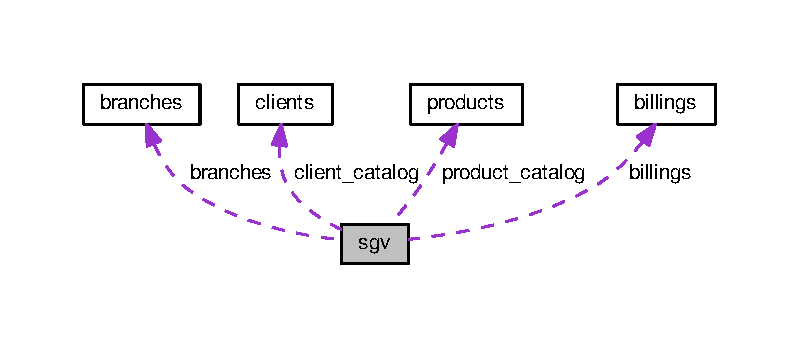
\includegraphics[width=350pt]{structsgv__coll__graph}
\end{center}
\end{figure}
\subsection*{Atributos Públicos}
\begin{DoxyCompactItemize}
\item 
\hyperlink{structclients}{Clients} \hyperlink{structsgv_ac28c11a53701c92a0133867d5790d3ab}{client\+\_\+catalog}
\item 
\hyperlink{structproducts}{Products} \hyperlink{structsgv_a614c60f5fb7c10e8e32928bba3b86277}{product\+\_\+catalog}
\item 
\hyperlink{structbillings}{Billings} \hyperlink{structsgv_a6fccce3e0a304bd96c165dac09f7a9ad}{billings}
\item 
\hyperlink{structbranches}{Branches} \hyperlink{structsgv_a655e9a2713e0baa6cfbaca8b84128616}{branches}
\end{DoxyCompactItemize}


\subsection{Documentação dos dados membro}
\mbox{\Hypertarget{structsgv_a6fccce3e0a304bd96c165dac09f7a9ad}\label{structsgv_a6fccce3e0a304bd96c165dac09f7a9ad}} 
\index{sgv@{sgv}!billings@{billings}}
\index{billings@{billings}!sgv@{sgv}}
\subsubsection{\texorpdfstring{billings}{billings}}
{\footnotesize\ttfamily \hyperlink{structbillings}{Billings} sgv\+::billings}

Cátalogo de faturação \mbox{\Hypertarget{structsgv_a655e9a2713e0baa6cfbaca8b84128616}\label{structsgv_a655e9a2713e0baa6cfbaca8b84128616}} 
\index{sgv@{sgv}!branches@{branches}}
\index{branches@{branches}!sgv@{sgv}}
\subsubsection{\texorpdfstring{branches}{branches}}
{\footnotesize\ttfamily \hyperlink{structbranches}{Branches} sgv\+::branches}

Cátalogo de filiais \mbox{\Hypertarget{structsgv_ac28c11a53701c92a0133867d5790d3ab}\label{structsgv_ac28c11a53701c92a0133867d5790d3ab}} 
\index{sgv@{sgv}!client\+\_\+catalog@{client\+\_\+catalog}}
\index{client\+\_\+catalog@{client\+\_\+catalog}!sgv@{sgv}}
\subsubsection{\texorpdfstring{client\+\_\+catalog}{client\_catalog}}
{\footnotesize\ttfamily \hyperlink{structclients}{Clients} sgv\+::client\+\_\+catalog}

Cátalogo de clientes \mbox{\Hypertarget{structsgv_a614c60f5fb7c10e8e32928bba3b86277}\label{structsgv_a614c60f5fb7c10e8e32928bba3b86277}} 
\index{sgv@{sgv}!product\+\_\+catalog@{product\+\_\+catalog}}
\index{product\+\_\+catalog@{product\+\_\+catalog}!sgv@{sgv}}
\subsubsection{\texorpdfstring{product\+\_\+catalog}{product\_catalog}}
{\footnotesize\ttfamily \hyperlink{structproducts}{Products} sgv\+::product\+\_\+catalog}

Cátalogo de produto 

A documentação para esta estrutura foi gerada a partir do seguinte ficheiro\+:\begin{DoxyCompactItemize}
\item 
src/sgv.\+c\end{DoxyCompactItemize}

\hypertarget{structstartValues}{}\section{Referência à estrutura start\+Values}
\label{structstartValues}\index{start\+Values@{start\+Values}}
\subsection*{Atributos Públicos}
\begin{DoxyCompactItemize}
\item 
G\+String $\ast$ \hyperlink{structstartValues_a378cbec9caa0421436f7395535ed8dc8}{path\+\_\+clients}
\item 
G\+String $\ast$ \hyperlink{structstartValues_a565548dbdb1349b7bf63b00f86d7d231}{path\+\_\+products}
\item 
G\+String $\ast$ \hyperlink{structstartValues_a8de24ef63dba39c2fe312a04f47654d0}{path\+\_\+sales}
\item 
gint \hyperlink{structstartValues_aaa0344a5400c6c8143eb52e3b31bf337}{valid\+\_\+clients}
\item 
gint \hyperlink{structstartValues_ac489314bf5f33955dc8b0d6233653787}{read\+\_\+clients}
\item 
gint \hyperlink{structstartValues_a5ff53c4c14ef84d2e7c8e399fc17cf4c}{valid\+\_\+products}
\item 
gint \hyperlink{structstartValues_a3ef4f4c6de7029cd5bbd297334de5454}{read\+\_\+products}
\item 
gint \hyperlink{structstartValues_a5f9fab3890b3551496940dda2b6f9154}{valid\+\_\+sales}
\item 
gint \hyperlink{structstartValues_a407924d22b3d5f4cdd94b8e8b0d3edd3}{read\+\_\+sales}
\end{DoxyCompactItemize}


\subsection{Documentação dos dados membro}
\mbox{\Hypertarget{structstartValues_a378cbec9caa0421436f7395535ed8dc8}\label{structstartValues_a378cbec9caa0421436f7395535ed8dc8}} 
\index{start\+Values@{start\+Values}!path\+\_\+clients@{path\+\_\+clients}}
\index{path\+\_\+clients@{path\+\_\+clients}!start\+Values@{start\+Values}}
\subsubsection{\texorpdfstring{path\+\_\+clients}{path\_clients}}
{\footnotesize\ttfamily G\+String$\ast$ start\+Values\+::path\+\_\+clients}

Path de ficheiro de clientes \mbox{\Hypertarget{structstartValues_a565548dbdb1349b7bf63b00f86d7d231}\label{structstartValues_a565548dbdb1349b7bf63b00f86d7d231}} 
\index{start\+Values@{start\+Values}!path\+\_\+products@{path\+\_\+products}}
\index{path\+\_\+products@{path\+\_\+products}!start\+Values@{start\+Values}}
\subsubsection{\texorpdfstring{path\+\_\+products}{path\_products}}
{\footnotesize\ttfamily G\+String$\ast$ start\+Values\+::path\+\_\+products}

Path de ficheiro de clientes \mbox{\Hypertarget{structstartValues_a8de24ef63dba39c2fe312a04f47654d0}\label{structstartValues_a8de24ef63dba39c2fe312a04f47654d0}} 
\index{start\+Values@{start\+Values}!path\+\_\+sales@{path\+\_\+sales}}
\index{path\+\_\+sales@{path\+\_\+sales}!start\+Values@{start\+Values}}
\subsubsection{\texorpdfstring{path\+\_\+sales}{path\_sales}}
{\footnotesize\ttfamily G\+String$\ast$ start\+Values\+::path\+\_\+sales}

Path de ficheiro de clientes \mbox{\Hypertarget{structstartValues_ac489314bf5f33955dc8b0d6233653787}\label{structstartValues_ac489314bf5f33955dc8b0d6233653787}} 
\index{start\+Values@{start\+Values}!read\+\_\+clients@{read\+\_\+clients}}
\index{read\+\_\+clients@{read\+\_\+clients}!start\+Values@{start\+Values}}
\subsubsection{\texorpdfstring{read\+\_\+clients}{read\_clients}}
{\footnotesize\ttfamily gint start\+Values\+::read\+\_\+clients}

Número de clientes lidos \mbox{\Hypertarget{structstartValues_a3ef4f4c6de7029cd5bbd297334de5454}\label{structstartValues_a3ef4f4c6de7029cd5bbd297334de5454}} 
\index{start\+Values@{start\+Values}!read\+\_\+products@{read\+\_\+products}}
\index{read\+\_\+products@{read\+\_\+products}!start\+Values@{start\+Values}}
\subsubsection{\texorpdfstring{read\+\_\+products}{read\_products}}
{\footnotesize\ttfamily gint start\+Values\+::read\+\_\+products}

Número de produtos lidos \mbox{\Hypertarget{structstartValues_a407924d22b3d5f4cdd94b8e8b0d3edd3}\label{structstartValues_a407924d22b3d5f4cdd94b8e8b0d3edd3}} 
\index{start\+Values@{start\+Values}!read\+\_\+sales@{read\+\_\+sales}}
\index{read\+\_\+sales@{read\+\_\+sales}!start\+Values@{start\+Values}}
\subsubsection{\texorpdfstring{read\+\_\+sales}{read\_sales}}
{\footnotesize\ttfamily gint start\+Values\+::read\+\_\+sales}

Número de vendas lidas \mbox{\Hypertarget{structstartValues_aaa0344a5400c6c8143eb52e3b31bf337}\label{structstartValues_aaa0344a5400c6c8143eb52e3b31bf337}} 
\index{start\+Values@{start\+Values}!valid\+\_\+clients@{valid\+\_\+clients}}
\index{valid\+\_\+clients@{valid\+\_\+clients}!start\+Values@{start\+Values}}
\subsubsection{\texorpdfstring{valid\+\_\+clients}{valid\_clients}}
{\footnotesize\ttfamily gint start\+Values\+::valid\+\_\+clients}

Número de clientes válidos \mbox{\Hypertarget{structstartValues_a5ff53c4c14ef84d2e7c8e399fc17cf4c}\label{structstartValues_a5ff53c4c14ef84d2e7c8e399fc17cf4c}} 
\index{start\+Values@{start\+Values}!valid\+\_\+products@{valid\+\_\+products}}
\index{valid\+\_\+products@{valid\+\_\+products}!start\+Values@{start\+Values}}
\subsubsection{\texorpdfstring{valid\+\_\+products}{valid\_products}}
{\footnotesize\ttfamily gint start\+Values\+::valid\+\_\+products}

Número de produtos válidos \mbox{\Hypertarget{structstartValues_a5f9fab3890b3551496940dda2b6f9154}\label{structstartValues_a5f9fab3890b3551496940dda2b6f9154}} 
\index{start\+Values@{start\+Values}!valid\+\_\+sales@{valid\+\_\+sales}}
\index{valid\+\_\+sales@{valid\+\_\+sales}!start\+Values@{start\+Values}}
\subsubsection{\texorpdfstring{valid\+\_\+sales}{valid\_sales}}
{\footnotesize\ttfamily gint start\+Values\+::valid\+\_\+sales}

Número de vendas válidas 

A documentação para esta estrutura foi gerada a partir do seguinte ficheiro\+:\begin{DoxyCompactItemize}
\item 
src/sgv.\+c\end{DoxyCompactItemize}

\chapter{Documentação do ficheiro}
\hypertarget{args_8h}{}\section{Referência ao ficheiro include/args.h}
\label{args_8h}\index{include/args.\+h@{include/args.\+h}}


Módulo de testes.  


Este grafo mostra quais são os ficheiros que incluem directamente ou indirectamente este ficheiro\+:
\nopagebreak
\begin{figure}[H]
\begin{center}
\leavevmode
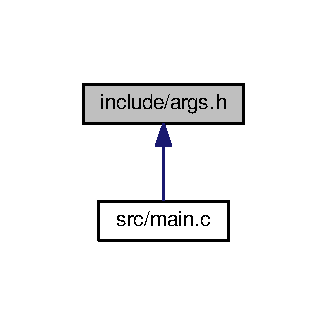
\includegraphics[width=157pt]{args_8h__dep__incl}
\end{center}
\end{figure}
\subsection*{Funções}
\begin{DoxyCompactItemize}
\item 
void \hyperlink{args_8h_a52171f656b6faaeb8dcf9811f32fca41}{start\+Input} (int, char $\ast$\mbox{[}$\,$\mbox{]})
\begin{DoxyCompactList}\small\item\em Imprimir o menu. \end{DoxyCompactList}\end{DoxyCompactItemize}


\subsection{Descrição detalhada}
Módulo de testes. 



\subsection{Documentação das funções}
\mbox{\Hypertarget{args_8h_a52171f656b6faaeb8dcf9811f32fca41}\label{args_8h_a52171f656b6faaeb8dcf9811f32fca41}} 
\index{args.\+h@{args.\+h}!start\+Input@{start\+Input}}
\index{start\+Input@{start\+Input}!args.\+h@{args.\+h}}
\subsubsection{\texorpdfstring{start\+Input()}{startInput()}}
{\footnotesize\ttfamily void start\+Input (\begin{DoxyParamCaption}\item[{int}]{,  }\item[{char $\ast$}]{\mbox{[}$\,$\mbox{]} }\end{DoxyParamCaption})}



Imprimir o menu. 


\begin{DoxyParams}{Parâmetros}
{\em n} & Número de argumentos \\
\hline
{\em args} & Array de argumentos \\
\hline
\end{DoxyParams}

\hypertarget{billing_8h}{}\section{Referência ao ficheiro include/billing.h}
\label{billing_8h}\index{include/billing.\+h@{include/billing.\+h}}


Módulo de tratamento de faturas.  


{\ttfamily \#include \char`\"{}info.\+h\char`\"{}}\newline
Diagrama de dependências de inclusão para billing.\+h\+:
\nopagebreak
\begin{figure}[H]
\begin{center}
\leavevmode
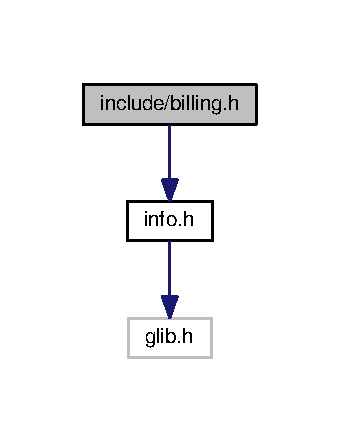
\includegraphics[width=163pt]{billing_8h__incl}
\end{center}
\end{figure}
Este grafo mostra quais são os ficheiros que incluem directamente ou indirectamente este ficheiro\+:
\nopagebreak
\begin{figure}[H]
\begin{center}
\leavevmode
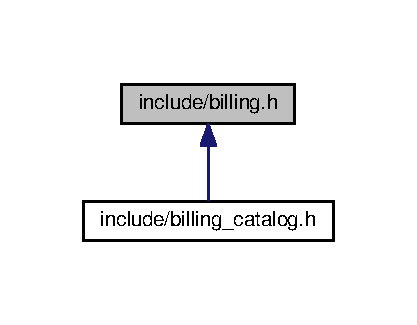
\includegraphics[width=200pt]{billing_8h__dep__incl}
\end{center}
\end{figure}
\subsection*{Definições de tipos}
\begin{DoxyCompactItemize}
\item 
\mbox{\Hypertarget{billing_8h_a40a581a33119b706e868e644e95e567c}\label{billing_8h_a40a581a33119b706e868e644e95e567c}} 
typedef struct \hyperlink{structbilling}{billing} $\ast$ {\bfseries Billing}
\item 
\mbox{\Hypertarget{billing_8h_a4a58018f639722d94776206880037321}\label{billing_8h_a4a58018f639722d94776206880037321}} 
typedef struct \hyperlink{structbillingProduct}{billing\+Product} $\ast$ {\bfseries Billing\+Product}
\end{DoxyCompactItemize}
\subsection*{Funções}
\begin{DoxyCompactItemize}
\item 
\hyperlink{structbilling}{Billing} \hyperlink{billing_8h_a2299512ec0acc1a36ba7a8e03552cd1a}{init\+Billing} ()
\begin{DoxyCompactList}\small\item\em Inicialização da estrutura Billing. \end{DoxyCompactList}\item 
\hyperlink{structbillingProduct}{Billing\+Product} \hyperlink{billing_8h_a929099ac8403e2f7f7f45d72e0c13c10}{init\+Billing\+Product} ()
\begin{DoxyCompactList}\small\item\em Inicialização da estrutura Billing\+Product. \end{DoxyCompactList}\item 
double $\ast$ \hyperlink{billing_8h_a80d7864adbd1c9772c9c45da2610f1ed}{get\+Product\+Values\+By\+Month\+Billing} (\hyperlink{structbilling}{Billing}, char $\ast$, int)
\begin{DoxyCompactList}\small\item\em De um array de inteiros, mostra ao utilizador o conteúdo numa tabela. \end{DoxyCompactList}\item 
int \hyperlink{billing_8h_a5516a70b8e4955173fb2d7e28b8b9403}{add\+Billing\+Product} (\hyperlink{structbilling}{Billing}, char $\ast$)
\begin{DoxyCompactList}\small\item\em Adiciona a estrutura Billing\+Product á hashtable billings\+Product. \end{DoxyCompactList}\item 
void \hyperlink{billing_8h_a0c67b429c7c3a636c91404797e2c5629}{update\+Billing} (\hyperlink{structbilling}{Billing}, char $\ast$, double, int, char, int)
\begin{DoxyCompactList}\small\item\em Atualiza os valores da estrutura Billing. \end{DoxyCompactList}\item 
int \hyperlink{billing_8h_a0864ada4fdc9399365a85de541a3c35f}{update\+Billing\+Product} (\hyperlink{structbillingProduct}{Billing\+Product}, double, int, char, int)
\begin{DoxyCompactList}\small\item\em Atualiza os valores da estrutura Billing\+Product. \end{DoxyCompactList}\item 
\hyperlink{structbillingProduct}{Billing\+Product} \hyperlink{billing_8h_ab9103789660d34fc3ce5a08522a100f5}{get\+Billing\+Product} (\hyperlink{structbilling}{Billing}, char $\ast$)
\begin{DoxyCompactList}\small\item\em Devolve Billing\+Product de um certo código de produto. \end{DoxyCompactList}\item 
double \hyperlink{billing_8h_a4a322fb422a93e1309e7683186a6a27a}{get\+Total\+Billed\+Billing} (\hyperlink{structbilling}{Billing})
\begin{DoxyCompactList}\small\item\em Devolve o total faturado no total. \end{DoxyCompactList}\item 
double \hyperlink{billing_8h_a6d408d0ee145fdc3704e95d48cc42b08}{get\+Total\+Billed\+N\+\_\+\+BP} (\hyperlink{structbillingProduct}{Billing\+Product})
\begin{DoxyCompactList}\small\item\em Devolve o valor faturado com o Tipo P. \end{DoxyCompactList}\item 
char $\ast$ \hyperlink{billing_8h_a4c650db3bc0b19c8aaefc046ef20280c}{get\+First\+Key} (\hyperlink{structbilling}{Billing})
\begin{DoxyCompactList}\small\item\em Devolve um código de produto. \end{DoxyCompactList}\item 
void \hyperlink{billing_8h_a2784c0282918ec01686e354c7afaa291}{update\+Totals\+From\+Billing} (\hyperlink{structbilling}{Billing}, \hyperlink{structquerie8Aux}{Query8\+Aux})
\begin{DoxyCompactList}\small\item\em Atualiza a estrutura Query8\+Aux com os valores de unidades de todas as filiais. \end{DoxyCompactList}\item 
void \hyperlink{billing_8h_aa10404871dc9c3a37b1d9fa8cd274bae}{free\+Billing\+Product} (\hyperlink{structbillingProduct}{Billing\+Product})
\begin{DoxyCompactList}\small\item\em Libertação da estrutura Billing\+Product. \end{DoxyCompactList}\item 
void \hyperlink{billing_8h_a401e050ba2fff2745debc4009d593de4}{free\+Billing} (\hyperlink{structbilling}{Billing})
\begin{DoxyCompactList}\small\item\em Libertação da estrutura Billing. \end{DoxyCompactList}\end{DoxyCompactItemize}


\subsection{Descrição detalhada}
Módulo de tratamento de faturas. 



\subsection{Documentação das funções}
\mbox{\Hypertarget{billing_8h_a5516a70b8e4955173fb2d7e28b8b9403}\label{billing_8h_a5516a70b8e4955173fb2d7e28b8b9403}} 
\index{billing.\+h@{billing.\+h}!add\+Billing\+Product@{add\+Billing\+Product}}
\index{add\+Billing\+Product@{add\+Billing\+Product}!billing.\+h@{billing.\+h}}
\subsubsection{\texorpdfstring{add\+Billing\+Product()}{addBillingProduct()}}
{\footnotesize\ttfamily int add\+Billing\+Product (\begin{DoxyParamCaption}\item[{\hyperlink{structbilling}{Billing}}]{,  }\item[{char $\ast$}]{ }\end{DoxyParamCaption})}



Adiciona a estrutura Billing\+Product á hashtable billings\+Product. 


\begin{DoxyParams}{Parâmetros}
{\em billing} & Estrutura Billing \\
\hline
{\em code} & Código de produto \\
\hline
\end{DoxyParams}
\begin{DoxyReturn}{Retorna}
int Resultado binário para detetar erros 
\end{DoxyReturn}
\mbox{\Hypertarget{billing_8h_a401e050ba2fff2745debc4009d593de4}\label{billing_8h_a401e050ba2fff2745debc4009d593de4}} 
\index{billing.\+h@{billing.\+h}!free\+Billing@{free\+Billing}}
\index{free\+Billing@{free\+Billing}!billing.\+h@{billing.\+h}}
\subsubsection{\texorpdfstring{free\+Billing()}{freeBilling()}}
{\footnotesize\ttfamily void free\+Billing (\begin{DoxyParamCaption}\item[{\hyperlink{structbilling}{Billing}}]{ }\end{DoxyParamCaption})}



Libertação da estrutura Billing. 


\begin{DoxyParams}{Parâmetros}
{\em billing} & estrutura Billing. \\
\hline
\end{DoxyParams}
\mbox{\Hypertarget{billing_8h_aa10404871dc9c3a37b1d9fa8cd274bae}\label{billing_8h_aa10404871dc9c3a37b1d9fa8cd274bae}} 
\index{billing.\+h@{billing.\+h}!free\+Billing\+Product@{free\+Billing\+Product}}
\index{free\+Billing\+Product@{free\+Billing\+Product}!billing.\+h@{billing.\+h}}
\subsubsection{\texorpdfstring{free\+Billing\+Product()}{freeBillingProduct()}}
{\footnotesize\ttfamily void free\+Billing\+Product (\begin{DoxyParamCaption}\item[{\hyperlink{structbillingProduct}{Billing\+Product}}]{ }\end{DoxyParamCaption})}



Libertação da estrutura Billing\+Product. 


\begin{DoxyParams}{Parâmetros}
{\em \hyperlink{structbillingProduct}{billing\+Product}} & estrutura Billing\+Product. \\
\hline
\end{DoxyParams}
\mbox{\Hypertarget{billing_8h_ab9103789660d34fc3ce5a08522a100f5}\label{billing_8h_ab9103789660d34fc3ce5a08522a100f5}} 
\index{billing.\+h@{billing.\+h}!get\+Billing\+Product@{get\+Billing\+Product}}
\index{get\+Billing\+Product@{get\+Billing\+Product}!billing.\+h@{billing.\+h}}
\subsubsection{\texorpdfstring{get\+Billing\+Product()}{getBillingProduct()}}
{\footnotesize\ttfamily \hyperlink{structbillingProduct}{Billing\+Product} get\+Billing\+Product (\begin{DoxyParamCaption}\item[{\hyperlink{structbilling}{Billing}}]{,  }\item[{char $\ast$}]{ }\end{DoxyParamCaption})}



Devolve Billing\+Product de um certo código de produto. 


\begin{DoxyParams}{Parâmetros}
{\em billing} & Estrutura Billing \\
\hline
{\em product\+\_\+code} & Código de produto \\
\hline
\end{DoxyParams}
\begin{DoxyReturn}{Retorna}
Billing\+Product Estrutura Billing\+Product 
\end{DoxyReturn}
\mbox{\Hypertarget{billing_8h_a4c650db3bc0b19c8aaefc046ef20280c}\label{billing_8h_a4c650db3bc0b19c8aaefc046ef20280c}} 
\index{billing.\+h@{billing.\+h}!get\+First\+Key@{get\+First\+Key}}
\index{get\+First\+Key@{get\+First\+Key}!billing.\+h@{billing.\+h}}
\subsubsection{\texorpdfstring{get\+First\+Key()}{getFirstKey()}}
{\footnotesize\ttfamily char$\ast$ get\+First\+Key (\begin{DoxyParamCaption}\item[{\hyperlink{structbilling}{Billing}}]{ }\end{DoxyParamCaption})}



Devolve um código de produto. 


\begin{DoxyParams}{Parâmetros}
{\em billing} & Estrutura Billing \\
\hline
\end{DoxyParams}
\begin{DoxyReturn}{Retorna}
char$\ast$ Código de produto 
\end{DoxyReturn}
\mbox{\Hypertarget{billing_8h_a80d7864adbd1c9772c9c45da2610f1ed}\label{billing_8h_a80d7864adbd1c9772c9c45da2610f1ed}} 
\index{billing.\+h@{billing.\+h}!get\+Product\+Values\+By\+Month\+Billing@{get\+Product\+Values\+By\+Month\+Billing}}
\index{get\+Product\+Values\+By\+Month\+Billing@{get\+Product\+Values\+By\+Month\+Billing}!billing.\+h@{billing.\+h}}
\subsubsection{\texorpdfstring{get\+Product\+Values\+By\+Month\+Billing()}{getProductValuesByMonthBilling()}}
{\footnotesize\ttfamily double$\ast$ get\+Product\+Values\+By\+Month\+Billing (\begin{DoxyParamCaption}\item[{\hyperlink{structbilling}{Billing}}]{,  }\item[{char $\ast$}]{,  }\item[{int}]{ }\end{DoxyParamCaption})}



De um array de inteiros, mostra ao utilizador o conteúdo numa tabela. 


\begin{DoxyParams}{Parâmetros}
{\em billing} & estrutura Billing \\
\hline
{\em product\+\_\+code} & Código do produto ao qual as faturas estão relacionadas \\
\hline
{\em branch} & numero da filial escolhida \\
\hline
\end{DoxyParams}
\begin{DoxyReturn}{Retorna}
double$\ast$ devolve uma lista de valores com quantidades e faturação numa dada filial 
\end{DoxyReturn}
\mbox{\Hypertarget{billing_8h_a4a322fb422a93e1309e7683186a6a27a}\label{billing_8h_a4a322fb422a93e1309e7683186a6a27a}} 
\index{billing.\+h@{billing.\+h}!get\+Total\+Billed\+Billing@{get\+Total\+Billed\+Billing}}
\index{get\+Total\+Billed\+Billing@{get\+Total\+Billed\+Billing}!billing.\+h@{billing.\+h}}
\subsubsection{\texorpdfstring{get\+Total\+Billed\+Billing()}{getTotalBilledBilling()}}
{\footnotesize\ttfamily double get\+Total\+Billed\+Billing (\begin{DoxyParamCaption}\item[{\hyperlink{structbilling}{Billing}}]{ }\end{DoxyParamCaption})}



Devolve o total faturado no total. 


\begin{DoxyParams}{Parâmetros}
{\em billing} & Estrutura Billing \\
\hline
\end{DoxyParams}
\begin{DoxyReturn}{Retorna}
double Valor faturado 
\end{DoxyReturn}
\mbox{\Hypertarget{billing_8h_a6d408d0ee145fdc3704e95d48cc42b08}\label{billing_8h_a6d408d0ee145fdc3704e95d48cc42b08}} 
\index{billing.\+h@{billing.\+h}!get\+Total\+Billed\+N\+\_\+\+BP@{get\+Total\+Billed\+N\+\_\+\+BP}}
\index{get\+Total\+Billed\+N\+\_\+\+BP@{get\+Total\+Billed\+N\+\_\+\+BP}!billing.\+h@{billing.\+h}}
\subsubsection{\texorpdfstring{get\+Total\+Billed\+N\+\_\+\+B\+P()}{getTotalBilledN\_BP()}}
{\footnotesize\ttfamily double get\+Total\+Billed\+N\+\_\+\+BP (\begin{DoxyParamCaption}\item[{\hyperlink{structbillingProduct}{Billing\+Product}}]{ }\end{DoxyParamCaption})}



Devolve o valor faturado com o Tipo P. 


\begin{DoxyParams}{Parâmetros}
{\em \hyperlink{structbillingProduct}{billing\+Product}} & Estrutura Billing\+Product \\
\hline
\end{DoxyParams}
\begin{DoxyReturn}{Retorna}
double Valor faturado 
\end{DoxyReturn}
\mbox{\Hypertarget{billing_8h_a2299512ec0acc1a36ba7a8e03552cd1a}\label{billing_8h_a2299512ec0acc1a36ba7a8e03552cd1a}} 
\index{billing.\+h@{billing.\+h}!init\+Billing@{init\+Billing}}
\index{init\+Billing@{init\+Billing}!billing.\+h@{billing.\+h}}
\subsubsection{\texorpdfstring{init\+Billing()}{initBilling()}}
{\footnotesize\ttfamily \hyperlink{structbilling}{Billing} init\+Billing (\begin{DoxyParamCaption}{ }\end{DoxyParamCaption})}



Inicialização da estrutura Billing. 

\begin{DoxyReturn}{Retorna}
Billing devolve um Billing inicializado. 
\end{DoxyReturn}
\mbox{\Hypertarget{billing_8h_a929099ac8403e2f7f7f45d72e0c13c10}\label{billing_8h_a929099ac8403e2f7f7f45d72e0c13c10}} 
\index{billing.\+h@{billing.\+h}!init\+Billing\+Product@{init\+Billing\+Product}}
\index{init\+Billing\+Product@{init\+Billing\+Product}!billing.\+h@{billing.\+h}}
\subsubsection{\texorpdfstring{init\+Billing\+Product()}{initBillingProduct()}}
{\footnotesize\ttfamily \hyperlink{structbillingProduct}{Billing\+Product} init\+Billing\+Product (\begin{DoxyParamCaption}{ }\end{DoxyParamCaption})}



Inicialização da estrutura Billing\+Product. 

\begin{DoxyReturn}{Retorna}
Billing\+Product devolve um Billing\+Product inicializado. 
\end{DoxyReturn}
\mbox{\Hypertarget{billing_8h_a0c67b429c7c3a636c91404797e2c5629}\label{billing_8h_a0c67b429c7c3a636c91404797e2c5629}} 
\index{billing.\+h@{billing.\+h}!update\+Billing@{update\+Billing}}
\index{update\+Billing@{update\+Billing}!billing.\+h@{billing.\+h}}
\subsubsection{\texorpdfstring{update\+Billing()}{updateBilling()}}
{\footnotesize\ttfamily void update\+Billing (\begin{DoxyParamCaption}\item[{\hyperlink{structbilling}{Billing}}]{,  }\item[{char $\ast$}]{,  }\item[{double}]{,  }\item[{int}]{,  }\item[{char}]{,  }\item[{int}]{ }\end{DoxyParamCaption})}



Atualiza os valores da estrutura Billing. 


\begin{DoxyParams}{Parâmetros}
{\em billing} & Estrutura Billing \\
\hline
{\em code} & Código de produto \\
\hline
{\em total\+Billed} & Valor faturado \\
\hline
{\em unities} & Unidades vendidas \\
\hline
{\em promotion\+\_\+type} & Tipo de promoção \\
\hline
{\em branch} & Filial \\
\hline
\end{DoxyParams}
\mbox{\Hypertarget{billing_8h_a0864ada4fdc9399365a85de541a3c35f}\label{billing_8h_a0864ada4fdc9399365a85de541a3c35f}} 
\index{billing.\+h@{billing.\+h}!update\+Billing\+Product@{update\+Billing\+Product}}
\index{update\+Billing\+Product@{update\+Billing\+Product}!billing.\+h@{billing.\+h}}
\subsubsection{\texorpdfstring{update\+Billing\+Product()}{updateBillingProduct()}}
{\footnotesize\ttfamily int update\+Billing\+Product (\begin{DoxyParamCaption}\item[{\hyperlink{structbillingProduct}{Billing\+Product}}]{,  }\item[{double}]{,  }\item[{int}]{,  }\item[{char}]{,  }\item[{int}]{ }\end{DoxyParamCaption})}



Atualiza os valores da estrutura Billing\+Product. 


\begin{DoxyParams}{Parâmetros}
{\em \hyperlink{structbillingProduct}{billing\+Product}} & Estrutura Billing\+Product \\
\hline
{\em total\+Billed} & Valor faturado \\
\hline
{\em unities} & Unidades vendidas \\
\hline
{\em promotion\+\_\+type} & Tipo de promoção \\
\hline
{\em branch} & Filial \\
\hline
\end{DoxyParams}
\begin{DoxyReturn}{Retorna}
int Resultado binário para detetar erros 
\end{DoxyReturn}
\mbox{\Hypertarget{billing_8h_a2784c0282918ec01686e354c7afaa291}\label{billing_8h_a2784c0282918ec01686e354c7afaa291}} 
\index{billing.\+h@{billing.\+h}!update\+Totals\+From\+Billing@{update\+Totals\+From\+Billing}}
\index{update\+Totals\+From\+Billing@{update\+Totals\+From\+Billing}!billing.\+h@{billing.\+h}}
\subsubsection{\texorpdfstring{update\+Totals\+From\+Billing()}{updateTotalsFromBilling()}}
{\footnotesize\ttfamily void update\+Totals\+From\+Billing (\begin{DoxyParamCaption}\item[{\hyperlink{structbilling}{Billing}}]{,  }\item[{\hyperlink{structquerie8Aux}{Query8\+Aux}}]{ }\end{DoxyParamCaption})}



Atualiza a estrutura Query8\+Aux com os valores de unidades de todas as filiais. 


\begin{DoxyParams}{Parâmetros}
{\em billing} & Estrutura Billing \\
\hline
{\em aux} & Estrutura Query8\+Aux \\
\hline
\end{DoxyParams}

\hypertarget{billing__catalog_8h}{}\section{Referência ao ficheiro include/billing\+\_\+catalog.h}
\label{billing__catalog_8h}\index{include/billing\+\_\+catalog.\+h@{include/billing\+\_\+catalog.\+h}}


Módulo de tratamentos do catálogo de faturação.  


{\ttfamily \#include \char`\"{}billing.\+h\char`\"{}}\newline
{\ttfamily \#include \char`\"{}sale.\+h\char`\"{}}\newline
Diagrama de dependências de inclusão para billing\+\_\+catalog.\+h\+:
\nopagebreak
\begin{figure}[H]
\begin{center}
\leavevmode
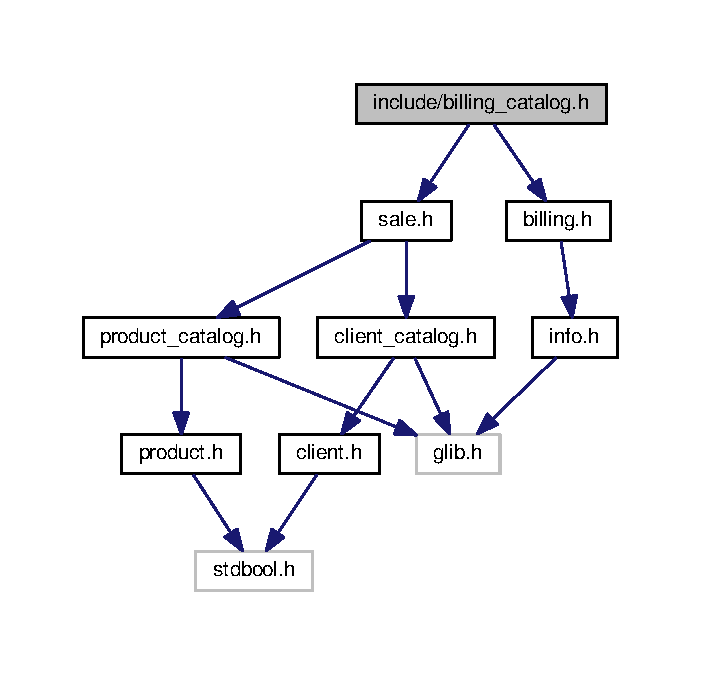
\includegraphics[width=337pt]{billing__catalog_8h__incl}
\end{center}
\end{figure}
\subsection*{Definições de tipos}
\begin{DoxyCompactItemize}
\item 
\mbox{\Hypertarget{billing__catalog_8h_aade9caed6d9b1b71171b58c7e12b5c59}\label{billing__catalog_8h_aade9caed6d9b1b71171b58c7e12b5c59}} 
typedef struct \hyperlink{structbillings}{billings} $\ast$ {\bfseries Billings}
\end{DoxyCompactItemize}
\subsection*{Funções}
\begin{DoxyCompactItemize}
\item 
\hyperlink{structbillings}{Billings} \hyperlink{billing__catalog_8h_a2462ff818495f6bd29a200f50454548d}{init\+Billings} ()
\begin{DoxyCompactList}\small\item\em Inicialização da estrutura Billing\+Product. \end{DoxyCompactList}\item 
double $\ast$ \hyperlink{billing__catalog_8h_a8f4c79c0806140d6111a7e3a0960e52c}{get\+Product\+Values\+By\+Month\+Billing\+Cat} (\hyperlink{structbillings}{Billings}, char $\ast$, int, int)
\begin{DoxyCompactList}\small\item\em Devolve um array de valores. \end{DoxyCompactList}\item 
void \hyperlink{billing__catalog_8h_a363a12fd71930d8571251fd1727f80c9}{add\+Billing} (\hyperlink{structbillings}{Billings}, \hyperlink{structbilling}{Billing}, int)
\begin{DoxyCompactList}\small\item\em Adiciona uma estrutura Billing á hashtable da estrutura Billings num certo mês. \end{DoxyCompactList}\item 
void \hyperlink{billing__catalog_8h_ac6d45af13bb32ef0a7296271ad6405ec}{update\+Billings} (\hyperlink{structbillings}{Billings}, \hyperlink{structsale}{Sale})
\begin{DoxyCompactList}\small\item\em Atualização dos valores da estrutura Billings. \end{DoxyCompactList}\item 
void \hyperlink{billing__catalog_8h_ad48fe031347c627b634eb885e291f261}{insert\+Billing\+Product} (\hyperlink{structbillings}{Billings}, int, char $\ast$)
\begin{DoxyCompactList}\small\item\em Insere uma estrutura Billing\+Product dentro de uma estrutura Billing. \end{DoxyCompactList}\item 
void \hyperlink{billing__catalog_8h_ac8160221943077610518c4f1e940509f}{destroy\+Billings} (\hyperlink{structbillings}{Billings})
\begin{DoxyCompactList}\small\item\em Liberta memória da estrutura Billings dada. \end{DoxyCompactList}\item 
\hyperlink{structquerie8Aux}{Query8\+Aux} \hyperlink{billing__catalog_8h_a136ebf0fd03ffba060034029cc0f5ebc}{get\+Totals\+From\+Billing\+Month\+Interval} (\hyperlink{structbillings}{Billings}, int, int)
\begin{DoxyCompactList}\small\item\em Devolve uma estrutura auxiliar Query8\+Aux com os valores de entre dois meses dados. \end{DoxyCompactList}\end{DoxyCompactItemize}


\subsection{Descrição detalhada}
Módulo de tratamentos do catálogo de faturação. 



\subsection{Documentação das funções}
\mbox{\Hypertarget{billing__catalog_8h_a363a12fd71930d8571251fd1727f80c9}\label{billing__catalog_8h_a363a12fd71930d8571251fd1727f80c9}} 
\index{billing\+\_\+catalog.\+h@{billing\+\_\+catalog.\+h}!add\+Billing@{add\+Billing}}
\index{add\+Billing@{add\+Billing}!billing\+\_\+catalog.\+h@{billing\+\_\+catalog.\+h}}
\subsubsection{\texorpdfstring{add\+Billing()}{addBilling()}}
{\footnotesize\ttfamily void add\+Billing (\begin{DoxyParamCaption}\item[{\hyperlink{structbillings}{Billings}}]{,  }\item[{\hyperlink{structbilling}{Billing}}]{,  }\item[{int}]{ }\end{DoxyParamCaption})}



Adiciona uma estrutura Billing á hashtable da estrutura Billings num certo mês. 


\begin{DoxyParams}{Parâmetros}
{\em billings} & Estrutura Billings \\
\hline
{\em billing} & Estrutura Billing \\
\hline
{\em month} & Número do mês \\
\hline
\end{DoxyParams}
\mbox{\Hypertarget{billing__catalog_8h_ac8160221943077610518c4f1e940509f}\label{billing__catalog_8h_ac8160221943077610518c4f1e940509f}} 
\index{billing\+\_\+catalog.\+h@{billing\+\_\+catalog.\+h}!destroy\+Billings@{destroy\+Billings}}
\index{destroy\+Billings@{destroy\+Billings}!billing\+\_\+catalog.\+h@{billing\+\_\+catalog.\+h}}
\subsubsection{\texorpdfstring{destroy\+Billings()}{destroyBillings()}}
{\footnotesize\ttfamily void destroy\+Billings (\begin{DoxyParamCaption}\item[{\hyperlink{structbillings}{Billings}}]{ }\end{DoxyParamCaption})}



Liberta memória da estrutura Billings dada. 


\begin{DoxyParams}{Parâmetros}
{\em bs} & Estrutura Billings \\
\hline
\end{DoxyParams}
\mbox{\Hypertarget{billing__catalog_8h_a8f4c79c0806140d6111a7e3a0960e52c}\label{billing__catalog_8h_a8f4c79c0806140d6111a7e3a0960e52c}} 
\index{billing\+\_\+catalog.\+h@{billing\+\_\+catalog.\+h}!get\+Product\+Values\+By\+Month\+Billing\+Cat@{get\+Product\+Values\+By\+Month\+Billing\+Cat}}
\index{get\+Product\+Values\+By\+Month\+Billing\+Cat@{get\+Product\+Values\+By\+Month\+Billing\+Cat}!billing\+\_\+catalog.\+h@{billing\+\_\+catalog.\+h}}
\subsubsection{\texorpdfstring{get\+Product\+Values\+By\+Month\+Billing\+Cat()}{getProductValuesByMonthBillingCat()}}
{\footnotesize\ttfamily double$\ast$ get\+Product\+Values\+By\+Month\+Billing\+Cat (\begin{DoxyParamCaption}\item[{\hyperlink{structbillings}{Billings}}]{,  }\item[{char $\ast$}]{,  }\item[{int}]{,  }\item[{int}]{ }\end{DoxyParamCaption})}



Devolve um array de valores. 


\begin{DoxyParams}{Parâmetros}
{\em bs} & \\
\hline
{\em product\+\_\+code} & Código de produto \\
\hline
{\em month} & Número do mês \\
\hline
{\em is\+Global} & Número usado para representar se é uma buscar global ou por filial \\
\hline
\end{DoxyParams}
\begin{DoxyReturn}{Retorna}
double$\ast$ devolve um Billing\+Product inicializado. 
\end{DoxyReturn}
\mbox{\Hypertarget{billing__catalog_8h_a136ebf0fd03ffba060034029cc0f5ebc}\label{billing__catalog_8h_a136ebf0fd03ffba060034029cc0f5ebc}} 
\index{billing\+\_\+catalog.\+h@{billing\+\_\+catalog.\+h}!get\+Totals\+From\+Billing\+Month\+Interval@{get\+Totals\+From\+Billing\+Month\+Interval}}
\index{get\+Totals\+From\+Billing\+Month\+Interval@{get\+Totals\+From\+Billing\+Month\+Interval}!billing\+\_\+catalog.\+h@{billing\+\_\+catalog.\+h}}
\subsubsection{\texorpdfstring{get\+Totals\+From\+Billing\+Month\+Interval()}{getTotalsFromBillingMonthInterval()}}
{\footnotesize\ttfamily \hyperlink{structquerie8Aux}{Query8\+Aux} get\+Totals\+From\+Billing\+Month\+Interval (\begin{DoxyParamCaption}\item[{\hyperlink{structbillings}{Billings}}]{,  }\item[{int}]{,  }\item[{int}]{ }\end{DoxyParamCaption})}



Devolve uma estrutura auxiliar Query8\+Aux com os valores de entre dois meses dados. 


\begin{DoxyParams}{Parâmetros}
{\em monthI} & Número de um mês \\
\hline
{\em monthF} & Número de um mês posterior ou igual a monthI \\
\hline
\end{DoxyParams}
\begin{DoxyReturn}{Retorna}
Query8\+Aux Uma estrutura Query8\+Aux 
\end{DoxyReturn}
\mbox{\Hypertarget{billing__catalog_8h_a2462ff818495f6bd29a200f50454548d}\label{billing__catalog_8h_a2462ff818495f6bd29a200f50454548d}} 
\index{billing\+\_\+catalog.\+h@{billing\+\_\+catalog.\+h}!init\+Billings@{init\+Billings}}
\index{init\+Billings@{init\+Billings}!billing\+\_\+catalog.\+h@{billing\+\_\+catalog.\+h}}
\subsubsection{\texorpdfstring{init\+Billings()}{initBillings()}}
{\footnotesize\ttfamily \hyperlink{structbillings}{Billings} init\+Billings (\begin{DoxyParamCaption}{ }\end{DoxyParamCaption})}



Inicialização da estrutura Billing\+Product. 

\begin{DoxyReturn}{Retorna}
Billings um Billing\+Product inicializado. 
\end{DoxyReturn}
\mbox{\Hypertarget{billing__catalog_8h_ad48fe031347c627b634eb885e291f261}\label{billing__catalog_8h_ad48fe031347c627b634eb885e291f261}} 
\index{billing\+\_\+catalog.\+h@{billing\+\_\+catalog.\+h}!insert\+Billing\+Product@{insert\+Billing\+Product}}
\index{insert\+Billing\+Product@{insert\+Billing\+Product}!billing\+\_\+catalog.\+h@{billing\+\_\+catalog.\+h}}
\subsubsection{\texorpdfstring{insert\+Billing\+Product()}{insertBillingProduct()}}
{\footnotesize\ttfamily void insert\+Billing\+Product (\begin{DoxyParamCaption}\item[{\hyperlink{structbillings}{Billings}}]{,  }\item[{int}]{,  }\item[{char $\ast$}]{ }\end{DoxyParamCaption})}



Insere uma estrutura Billing\+Product dentro de uma estrutura Billing. 


\begin{DoxyParams}{Parâmetros}
{\em bs} & Estrutura Billings \\
\hline
{\em month} & Número do mês \\
\hline
{\em product\+\_\+code} & Código de produto \\
\hline
\end{DoxyParams}
\mbox{\Hypertarget{billing__catalog_8h_ac6d45af13bb32ef0a7296271ad6405ec}\label{billing__catalog_8h_ac6d45af13bb32ef0a7296271ad6405ec}} 
\index{billing\+\_\+catalog.\+h@{billing\+\_\+catalog.\+h}!update\+Billings@{update\+Billings}}
\index{update\+Billings@{update\+Billings}!billing\+\_\+catalog.\+h@{billing\+\_\+catalog.\+h}}
\subsubsection{\texorpdfstring{update\+Billings()}{updateBillings()}}
{\footnotesize\ttfamily void update\+Billings (\begin{DoxyParamCaption}\item[{\hyperlink{structbillings}{Billings}}]{,  }\item[{\hyperlink{structsale}{Sale}}]{ }\end{DoxyParamCaption})}



Atualização dos valores da estrutura Billings. 


\begin{DoxyParams}{Parâmetros}
{\em bs} & Estrutura Billings \\
\hline
{\em sale} & Estrutura Sale \\
\hline
\end{DoxyParams}

\hypertarget{branch_8h}{}\section{Referência ao ficheiro include/branch.h}
\label{branch_8h}\index{include/branch.\+h@{include/branch.\+h}}


Módulo de tratamento de filiais.  


{\ttfamily \#include $<$glib.\+h$>$}\newline
{\ttfamily \#include \char`\"{}info.\+h\char`\"{}}\newline
Diagrama de dependências de inclusão para branch.\+h\+:
\nopagebreak
\begin{figure}[H]
\begin{center}
\leavevmode
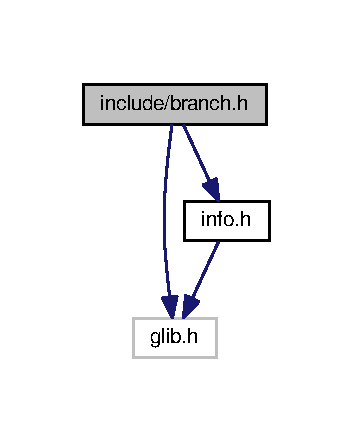
\includegraphics[width=170pt]{branch_8h__incl}
\end{center}
\end{figure}
Este grafo mostra quais são os ficheiros que incluem directamente ou indirectamente este ficheiro\+:
\nopagebreak
\begin{figure}[H]
\begin{center}
\leavevmode
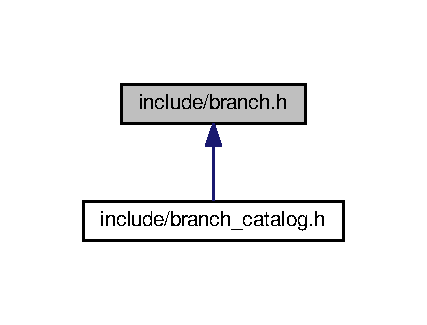
\includegraphics[width=205pt]{branch_8h__dep__incl}
\end{center}
\end{figure}
\subsection*{Definições de tipos}
\begin{DoxyCompactItemize}
\item 
\mbox{\Hypertarget{branch_8h_af8c19b0912e34d02318367931d7181b2}\label{branch_8h_af8c19b0912e34d02318367931d7181b2}} 
typedef struct \hyperlink{structbranch}{branch} $\ast$ {\bfseries Branch}
\item 
\mbox{\Hypertarget{branch_8h_ac97db6a6a68c37bf5f22477bb3afeb0f}\label{branch_8h_ac97db6a6a68c37bf5f22477bb3afeb0f}} 
typedef struct \hyperlink{structrelationWithClient}{relation\+With\+Client} $\ast$ {\bfseries Relation\+With\+Client}
\item 
\mbox{\Hypertarget{branch_8h_afeeb28940432c103763ff8a47cc3ffba}\label{branch_8h_afeeb28940432c103763ff8a47cc3ffba}} 
typedef struct \hyperlink{structrelationWithProduct}{relation\+With\+Product} $\ast$ {\bfseries Relation\+With\+Product}
\item 
\mbox{\Hypertarget{branch_8h_a6735cef113d089d30f0c4a58c7c12b48}\label{branch_8h_a6735cef113d089d30f0c4a58c7c12b48}} 
typedef struct \hyperlink{structinfoClient}{info\+Client} $\ast$ {\bfseries Info\+Client}
\item 
\mbox{\Hypertarget{branch_8h_a319fc1cc2ddf310d9d244be9f229b619}\label{branch_8h_a319fc1cc2ddf310d9d244be9f229b619}} 
typedef struct \hyperlink{structinfoProduct}{info\+Product} $\ast$ {\bfseries Info\+Product}
\end{DoxyCompactItemize}
\subsection*{Funções}
\begin{DoxyCompactItemize}
\item 
\hyperlink{structbranch}{Branch} \hyperlink{branch_8h_ab78dddaa4a96b4011d6f415746225189}{init\+Branch} ()
\begin{DoxyCompactList}\small\item\em Inicialização da estrutura Branch. \end{DoxyCompactList}\item 
\hyperlink{structrelationWithClient}{Relation\+With\+Client} \hyperlink{branch_8h_ac5fa333061542fca1ce1686355abd297}{init\+Relation\+With\+Client} ()
\begin{DoxyCompactList}\small\item\em Inicialização da estrutura Relation\+With\+Client. \end{DoxyCompactList}\item 
\hyperlink{structrelationWithProduct}{Relation\+With\+Product} \hyperlink{branch_8h_ab557c0d331a056c473fb8795966f004c}{init\+Relation\+With\+Product} ()
\begin{DoxyCompactList}\small\item\em Inicialização da estrutura Relation\+With\+Product. \end{DoxyCompactList}\item 
\hyperlink{structinfoClient}{Info\+Client} \hyperlink{branch_8h_a29943b5d792ca02c20695f79322d3566}{init\+Info\+Client} ()
\begin{DoxyCompactList}\small\item\em Inicialização da estrutura Info\+Client. \end{DoxyCompactList}\item 
\hyperlink{structinfoProduct}{Info\+Product} \hyperlink{branch_8h_a6c25b0d0a9c6725f789053fe39ebcbe6}{init\+Info\+Product} ()
\begin{DoxyCompactList}\small\item\em Inicialização da estrutura Info\+Product. \end{DoxyCompactList}\item 
void \hyperlink{branch_8h_ac744aa1cfc60436a485fc8dfa969baa6}{add\+Relation\+With\+Client} (\hyperlink{structbranch}{Branch}, char $\ast$, \hyperlink{structrelationWithClient}{Relation\+With\+Client})
\begin{DoxyCompactList}\small\item\em Adiciona a estrutura \hyperlink{structrelationWithClient}{relation\+With\+Client} á hashtable presente na estrutura products\+Clients. \end{DoxyCompactList}\item 
void \hyperlink{branch_8h_ad2143c449df4aed38b1287a8ca3f401e}{add\+Relation\+With\+Product} (\hyperlink{structbranch}{Branch}, char $\ast$, \hyperlink{structrelationWithProduct}{Relation\+With\+Product})
\begin{DoxyCompactList}\small\item\em Adiciona a estrutura Relation\+With\+Product á hashtable presente na estrutura clients\+Products. \end{DoxyCompactList}\item 
void \hyperlink{branch_8h_a90038017270a7e2a6173b622d85e4fca}{add\+Info\+Client} (\hyperlink{structrelationWithClient}{Relation\+With\+Client}, char $\ast$, \hyperlink{structinfoClient}{Info\+Client})
\begin{DoxyCompactList}\small\item\em Adiciona a estrutura Info\+Client á hashtable presente na estrutura Relation\+With\+Client. \end{DoxyCompactList}\item 
void \hyperlink{branch_8h_a912757336621d994b8d67f30f664f9c6}{add\+Info\+Product} (\hyperlink{structrelationWithProduct}{Relation\+With\+Product}, char $\ast$, \hyperlink{structinfoProduct}{Info\+Product})
\begin{DoxyCompactList}\small\item\em Adiciona a estrutura Info\+Product á hashtable presente na estrutura Relation\+With\+Product. \end{DoxyCompactList}\item 
void \hyperlink{branch_8h_a931f0f0cff34b0fe29ae78f1b68906ea}{update\+Branch} (\hyperlink{structbranch}{Branch}, char $\ast$, char $\ast$, int, char, double, int)
\begin{DoxyCompactList}\small\item\em Atualizar os dados dentro da estrutura Branch. \end{DoxyCompactList}\item 
void \hyperlink{branch_8h_a64799b8adf1a03548a638b0ebf21a2a1}{update\+Relation\+With\+Product} (\hyperlink{structrelationWithProduct}{Relation\+With\+Product}, char $\ast$, int, double, int)
\begin{DoxyCompactList}\small\item\em Atualizar os dados dentro da estrutura Relation\+With\+Product. \end{DoxyCompactList}\item 
void \hyperlink{branch_8h_ac99a467c7cd0a0b057cca65322c263ba}{update\+Relation\+With\+Client} (\hyperlink{structrelationWithClient}{Relation\+With\+Client}, char $\ast$, int, char)
\begin{DoxyCompactList}\small\item\em Atualizar os dados dentro da estrutura Relation\+With\+Client. \end{DoxyCompactList}\item 
void \hyperlink{branch_8h_a05f090e58ed0ca388aaf715e21ac3f5b}{update\+Info\+Client} (\hyperlink{structinfoClient}{Info\+Client}, int, char)
\begin{DoxyCompactList}\small\item\em Atualizar os dados dentro da estrutura Info\+Client. \end{DoxyCompactList}\item 
void \hyperlink{branch_8h_a2d8b0277fb339acbe31447d2b5770b74}{update\+Info\+Product} (\hyperlink{structinfoProduct}{Info\+Product}, int, double, int)
\begin{DoxyCompactList}\small\item\em Atualizar os dados dentro da estrutura Info\+Product. \end{DoxyCompactList}\item 
void \hyperlink{branch_8h_a86840dde7a0d8f7b4810d4c60b736225}{free\+Branch} (\hyperlink{structbranch}{Branch})
\begin{DoxyCompactList}\small\item\em Libertação da estrutura Branch. \end{DoxyCompactList}\item 
void \hyperlink{branch_8h_aa01c84a5100588ff38385992e073d49b}{free\+Relation\+With\+Client} (\hyperlink{structrelationWithClient}{Relation\+With\+Client})
\begin{DoxyCompactList}\small\item\em Libertação da estrutura Relation\+With\+Client. \end{DoxyCompactList}\item 
void \hyperlink{branch_8h_a54776cb56477089cbf5471fb68d9a107}{free\+Relation\+With\+Product} (\hyperlink{structrelationWithProduct}{Relation\+With\+Product})
\begin{DoxyCompactList}\small\item\em Libertação da estrutura Relation\+With\+Product. \end{DoxyCompactList}\item 
void \hyperlink{branch_8h_ac6e5b41df3a4dbed7989c4284d1ce29b}{free\+Info\+Client} (\hyperlink{structinfoClient}{Info\+Client})
\begin{DoxyCompactList}\small\item\em Libertação da estrutura Info\+Client. \end{DoxyCompactList}\item 
void \hyperlink{branch_8h_a967e37aa236e84b2f0bca6ed6e07bf53}{free\+Info\+Product} (\hyperlink{structinfoProduct}{Info\+Product})
\begin{DoxyCompactList}\small\item\em Libertação da estrutura Info\+Product. \end{DoxyCompactList}\item 
char $\ast$$\ast$ \hyperlink{branch_8h_a9f46f1927c8d62fd2d12a65299fd3664}{get\+Client\+Codes} (\hyperlink{structbranch}{Branch}, int $\ast$)
\begin{DoxyCompactList}\small\item\em Devolve o array ordenado dos códigos de clientes que compraram numa certa filial. \end{DoxyCompactList}\item 
char $\ast$$\ast$ \hyperlink{branch_8h_af4d05aa5caebf392603ac1c1992caf64}{get\+Products\+In\+Branch} (\hyperlink{structbranch}{Branch})
\begin{DoxyCompactList}\small\item\em Devolve um array de códigos de produto vendidos numa certa filial. \end{DoxyCompactList}\item 
\hyperlink{structquerie9Aux}{Query9\+Aux} \hyperlink{branch_8h_aa7f2c2d5142aea9c5e721f2e6359b016}{product\+Bought\+By} (\hyperlink{structbranch}{Branch}, char $\ast$)
\begin{DoxyCompactList}\small\item\em Deolve uma estrutura Query9\+Aux com os valores especificos a um dado código de produto. \end{DoxyCompactList}\item 
char $\ast$$\ast$ \hyperlink{branch_8h_aad93869b82bee7ca2b7664b23249abad}{get\+Clients\+In\+Branch} (\hyperlink{structbranch}{Branch})
\begin{DoxyCompactList}\small\item\em Devolve um array com todos os códigos de cliente de uma certa filial. \end{DoxyCompactList}\item 
int $\ast$ \hyperlink{branch_8h_a5e77de75f66e6a972c118f99421f41e7}{get\+Client\+Shop\+Log} (\hyperlink{structbranch}{Branch}, char $\ast$)
\begin{DoxyCompactList}\small\item\em Devolve um array com as quantidades de produtos comprados em cada mês. \end{DoxyCompactList}\item 
void \hyperlink{branch_8h_ac74f0e45a7997a7e50c0dd431f1ed0c8}{get\+Most\+Bought\+By\+Branch} (\hyperlink{structbranch}{Branch}, char $\ast$, int, G\+Hash\+Table $\ast$)
\begin{DoxyCompactList}\small\item\em Atualiza Hashtable com key=código de produto e value=Estrutura Info. \end{DoxyCompactList}\item 
void \hyperlink{branch_8h_a75893dd876fe70c79f95a9b0e60038d9}{update\+N\+Most\+Bought} (\hyperlink{structbranch}{Branch}, G\+Hash\+Table $\ast$, int)
\begin{DoxyCompactList}\small\item\em Atualiza Hashtable com key=código de produto e value=Estrutura Aux. \end{DoxyCompactList}\item 
void \hyperlink{branch_8h_abe83a433aab46b449846fa0543efa2ba}{client\+Spent\+Most\+On\+Branch} (\hyperlink{structbranch}{Branch}, char $\ast$, G\+Hash\+Table $\ast$)
\begin{DoxyCompactList}\small\item\em Atualiza Hashtable com key=código de cliente e value=Estrutura Money. \end{DoxyCompactList}\item 
void \hyperlink{branch_8h_a6034e30ef92871c3f6e6c84690965620}{intersect\+Clients} (\hyperlink{structbranch}{Branch}, G\+Hash\+Table $\ast$)
\begin{DoxyCompactList}\small\item\em Remove todos os códigos de cliente que não compraram numa dada filial. \end{DoxyCompactList}\end{DoxyCompactItemize}


\subsection{Descrição detalhada}
Módulo de tratamento de filiais. 



\subsection{Documentação das funções}
\mbox{\Hypertarget{branch_8h_a90038017270a7e2a6173b622d85e4fca}\label{branch_8h_a90038017270a7e2a6173b622d85e4fca}} 
\index{branch.\+h@{branch.\+h}!add\+Info\+Client@{add\+Info\+Client}}
\index{add\+Info\+Client@{add\+Info\+Client}!branch.\+h@{branch.\+h}}
\subsubsection{\texorpdfstring{add\+Info\+Client()}{addInfoClient()}}
{\footnotesize\ttfamily void add\+Info\+Client (\begin{DoxyParamCaption}\item[{\hyperlink{structrelationWithClient}{Relation\+With\+Client}}]{,  }\item[{char $\ast$}]{,  }\item[{\hyperlink{structinfoClient}{Info\+Client}}]{ }\end{DoxyParamCaption})}



Adiciona a estrutura Info\+Client á hashtable presente na estrutura Relation\+With\+Client. 


\begin{DoxyParams}{Parâmetros}
{\em rcc} & Estrutura Relation\+With\+Client \\
\hline
{\em client\+\_\+code} & Código do cliente \\
\hline
{\em ic} & Estrutura Info\+Client \\
\hline
\end{DoxyParams}
\mbox{\Hypertarget{branch_8h_a912757336621d994b8d67f30f664f9c6}\label{branch_8h_a912757336621d994b8d67f30f664f9c6}} 
\index{branch.\+h@{branch.\+h}!add\+Info\+Product@{add\+Info\+Product}}
\index{add\+Info\+Product@{add\+Info\+Product}!branch.\+h@{branch.\+h}}
\subsubsection{\texorpdfstring{add\+Info\+Product()}{addInfoProduct()}}
{\footnotesize\ttfamily void add\+Info\+Product (\begin{DoxyParamCaption}\item[{\hyperlink{structrelationWithProduct}{Relation\+With\+Product}}]{,  }\item[{char $\ast$}]{,  }\item[{\hyperlink{structinfoProduct}{Info\+Product}}]{ }\end{DoxyParamCaption})}



Adiciona a estrutura Info\+Product á hashtable presente na estrutura Relation\+With\+Product. 


\begin{DoxyParams}{Parâmetros}
{\em rcp} & Estrutura Relation\+With\+Product \\
\hline
{\em product\+\_\+code} & Código do produto \\
\hline
{\em ip} & Estrutura Info\+Product \\
\hline
\end{DoxyParams}
\mbox{\Hypertarget{branch_8h_ac744aa1cfc60436a485fc8dfa969baa6}\label{branch_8h_ac744aa1cfc60436a485fc8dfa969baa6}} 
\index{branch.\+h@{branch.\+h}!add\+Relation\+With\+Client@{add\+Relation\+With\+Client}}
\index{add\+Relation\+With\+Client@{add\+Relation\+With\+Client}!branch.\+h@{branch.\+h}}
\subsubsection{\texorpdfstring{add\+Relation\+With\+Client()}{addRelationWithClient()}}
{\footnotesize\ttfamily void add\+Relation\+With\+Client (\begin{DoxyParamCaption}\item[{\hyperlink{structbranch}{Branch}}]{,  }\item[{char $\ast$}]{,  }\item[{\hyperlink{structrelationWithClient}{Relation\+With\+Client}}]{ }\end{DoxyParamCaption})}



Adiciona a estrutura \hyperlink{structrelationWithClient}{relation\+With\+Client} á hashtable presente na estrutura products\+Clients. 


\begin{DoxyParams}{Parâmetros}
{\em branch} & Estrutura Branch \\
\hline
{\em product\+\_\+code} & Código do produto \\
\hline
{\em rcc} & Estrutura Relation\+With\+Client \\
\hline
\end{DoxyParams}
\mbox{\Hypertarget{branch_8h_ad2143c449df4aed38b1287a8ca3f401e}\label{branch_8h_ad2143c449df4aed38b1287a8ca3f401e}} 
\index{branch.\+h@{branch.\+h}!add\+Relation\+With\+Product@{add\+Relation\+With\+Product}}
\index{add\+Relation\+With\+Product@{add\+Relation\+With\+Product}!branch.\+h@{branch.\+h}}
\subsubsection{\texorpdfstring{add\+Relation\+With\+Product()}{addRelationWithProduct()}}
{\footnotesize\ttfamily void add\+Relation\+With\+Product (\begin{DoxyParamCaption}\item[{\hyperlink{structbranch}{Branch}}]{,  }\item[{char $\ast$}]{,  }\item[{\hyperlink{structrelationWithProduct}{Relation\+With\+Product}}]{ }\end{DoxyParamCaption})}



Adiciona a estrutura Relation\+With\+Product á hashtable presente na estrutura clients\+Products. 


\begin{DoxyParams}{Parâmetros}
{\em branch} & Estrutura Branch \\
\hline
{\em client\+\_\+code} & Código do cliente \\
\hline
{\em rcp} & Estrutura Relation\+With\+Product \\
\hline
\end{DoxyParams}
\mbox{\Hypertarget{branch_8h_abe83a433aab46b449846fa0543efa2ba}\label{branch_8h_abe83a433aab46b449846fa0543efa2ba}} 
\index{branch.\+h@{branch.\+h}!client\+Spent\+Most\+On\+Branch@{client\+Spent\+Most\+On\+Branch}}
\index{client\+Spent\+Most\+On\+Branch@{client\+Spent\+Most\+On\+Branch}!branch.\+h@{branch.\+h}}
\subsubsection{\texorpdfstring{client\+Spent\+Most\+On\+Branch()}{clientSpentMostOnBranch()}}
{\footnotesize\ttfamily void client\+Spent\+Most\+On\+Branch (\begin{DoxyParamCaption}\item[{\hyperlink{structbranch}{Branch}}]{,  }\item[{char $\ast$}]{,  }\item[{G\+Hash\+Table $\ast$}]{ }\end{DoxyParamCaption})}



Atualiza Hashtable com key=código de cliente e value=Estrutura Money. 


\begin{DoxyParams}{Parâmetros}
{\em b} & Estrutura Branch \\
\hline
{\em client\+\_\+code} & Código do cliente \\
\hline
{\em \+\_\+max\+Spent} & Hashtable com códigos de clientes e os valores gastos o ano todo \\
\hline
\end{DoxyParams}
\mbox{\Hypertarget{branch_8h_a86840dde7a0d8f7b4810d4c60b736225}\label{branch_8h_a86840dde7a0d8f7b4810d4c60b736225}} 
\index{branch.\+h@{branch.\+h}!free\+Branch@{free\+Branch}}
\index{free\+Branch@{free\+Branch}!branch.\+h@{branch.\+h}}
\subsubsection{\texorpdfstring{free\+Branch()}{freeBranch()}}
{\footnotesize\ttfamily void free\+Branch (\begin{DoxyParamCaption}\item[{\hyperlink{structbranch}{Branch}}]{ }\end{DoxyParamCaption})}



Libertação da estrutura Branch. 


\begin{DoxyParams}{Parâmetros}
{\em branch} & Estrutura Branch a ser libertada \\
\hline
\end{DoxyParams}
\mbox{\Hypertarget{branch_8h_ac6e5b41df3a4dbed7989c4284d1ce29b}\label{branch_8h_ac6e5b41df3a4dbed7989c4284d1ce29b}} 
\index{branch.\+h@{branch.\+h}!free\+Info\+Client@{free\+Info\+Client}}
\index{free\+Info\+Client@{free\+Info\+Client}!branch.\+h@{branch.\+h}}
\subsubsection{\texorpdfstring{free\+Info\+Client()}{freeInfoClient()}}
{\footnotesize\ttfamily void free\+Info\+Client (\begin{DoxyParamCaption}\item[{\hyperlink{structinfoClient}{Info\+Client}}]{ }\end{DoxyParamCaption})}



Libertação da estrutura Info\+Client. 


\begin{DoxyParams}{Parâmetros}
{\em ic} & Estrutura Info\+Client a ser libertada \\
\hline
\end{DoxyParams}
\mbox{\Hypertarget{branch_8h_a967e37aa236e84b2f0bca6ed6e07bf53}\label{branch_8h_a967e37aa236e84b2f0bca6ed6e07bf53}} 
\index{branch.\+h@{branch.\+h}!free\+Info\+Product@{free\+Info\+Product}}
\index{free\+Info\+Product@{free\+Info\+Product}!branch.\+h@{branch.\+h}}
\subsubsection{\texorpdfstring{free\+Info\+Product()}{freeInfoProduct()}}
{\footnotesize\ttfamily void free\+Info\+Product (\begin{DoxyParamCaption}\item[{\hyperlink{structinfoProduct}{Info\+Product}}]{ }\end{DoxyParamCaption})}



Libertação da estrutura Info\+Product. 


\begin{DoxyParams}{Parâmetros}
{\em ip} & Estrutura Info\+Product a ser libertada \\
\hline
\end{DoxyParams}
\mbox{\Hypertarget{branch_8h_aa01c84a5100588ff38385992e073d49b}\label{branch_8h_aa01c84a5100588ff38385992e073d49b}} 
\index{branch.\+h@{branch.\+h}!free\+Relation\+With\+Client@{free\+Relation\+With\+Client}}
\index{free\+Relation\+With\+Client@{free\+Relation\+With\+Client}!branch.\+h@{branch.\+h}}
\subsubsection{\texorpdfstring{free\+Relation\+With\+Client()}{freeRelationWithClient()}}
{\footnotesize\ttfamily void free\+Relation\+With\+Client (\begin{DoxyParamCaption}\item[{\hyperlink{structrelationWithClient}{Relation\+With\+Client}}]{ }\end{DoxyParamCaption})}



Libertação da estrutura Relation\+With\+Client. 


\begin{DoxyParams}{Parâmetros}
{\em rc} & Estrutura Relation\+With\+Client a ser libertada \\
\hline
\end{DoxyParams}
\mbox{\Hypertarget{branch_8h_a54776cb56477089cbf5471fb68d9a107}\label{branch_8h_a54776cb56477089cbf5471fb68d9a107}} 
\index{branch.\+h@{branch.\+h}!free\+Relation\+With\+Product@{free\+Relation\+With\+Product}}
\index{free\+Relation\+With\+Product@{free\+Relation\+With\+Product}!branch.\+h@{branch.\+h}}
\subsubsection{\texorpdfstring{free\+Relation\+With\+Product()}{freeRelationWithProduct()}}
{\footnotesize\ttfamily void free\+Relation\+With\+Product (\begin{DoxyParamCaption}\item[{\hyperlink{structrelationWithProduct}{Relation\+With\+Product}}]{ }\end{DoxyParamCaption})}



Libertação da estrutura Relation\+With\+Product. 


\begin{DoxyParams}{Parâmetros}
{\em rp} & Estrutura Relation\+With\+Product a ser libertada \\
\hline
\end{DoxyParams}
\mbox{\Hypertarget{branch_8h_a9f46f1927c8d62fd2d12a65299fd3664}\label{branch_8h_a9f46f1927c8d62fd2d12a65299fd3664}} 
\index{branch.\+h@{branch.\+h}!get\+Client\+Codes@{get\+Client\+Codes}}
\index{get\+Client\+Codes@{get\+Client\+Codes}!branch.\+h@{branch.\+h}}
\subsubsection{\texorpdfstring{get\+Client\+Codes()}{getClientCodes()}}
{\footnotesize\ttfamily char$\ast$$\ast$ get\+Client\+Codes (\begin{DoxyParamCaption}\item[{\hyperlink{structbranch}{Branch}}]{,  }\item[{int $\ast$}]{ }\end{DoxyParamCaption})}



Devolve o array ordenado dos códigos de clientes que compraram numa certa filial. 


\begin{DoxyParams}{Parâmetros}
{\em branch} & Estrutura Branch \\
\hline
{\em n} & Número easter egg \\
\hline
\end{DoxyParams}
\begin{DoxyReturn}{Retorna}
char$\ast$$\ast$ Array ordenado dos códigos de clientes que compraram numa certa filial 
\end{DoxyReturn}
\mbox{\Hypertarget{branch_8h_a5e77de75f66e6a972c118f99421f41e7}\label{branch_8h_a5e77de75f66e6a972c118f99421f41e7}} 
\index{branch.\+h@{branch.\+h}!get\+Client\+Shop\+Log@{get\+Client\+Shop\+Log}}
\index{get\+Client\+Shop\+Log@{get\+Client\+Shop\+Log}!branch.\+h@{branch.\+h}}
\subsubsection{\texorpdfstring{get\+Client\+Shop\+Log()}{getClientShopLog()}}
{\footnotesize\ttfamily int$\ast$ get\+Client\+Shop\+Log (\begin{DoxyParamCaption}\item[{\hyperlink{structbranch}{Branch}}]{,  }\item[{char $\ast$}]{ }\end{DoxyParamCaption})}



Devolve um array com as quantidades de produtos comprados em cada mês. 


\begin{DoxyParams}{Parâmetros}
{\em b} & Estrutura Branch \\
\hline
{\em client\+\_\+code} & Código do cliente \\
\hline
\end{DoxyParams}
\begin{DoxyReturn}{Retorna}
int$\ast$ Array com quantidades de produtos comprados em cada mês 
\end{DoxyReturn}
\mbox{\Hypertarget{branch_8h_aad93869b82bee7ca2b7664b23249abad}\label{branch_8h_aad93869b82bee7ca2b7664b23249abad}} 
\index{branch.\+h@{branch.\+h}!get\+Clients\+In\+Branch@{get\+Clients\+In\+Branch}}
\index{get\+Clients\+In\+Branch@{get\+Clients\+In\+Branch}!branch.\+h@{branch.\+h}}
\subsubsection{\texorpdfstring{get\+Clients\+In\+Branch()}{getClientsInBranch()}}
{\footnotesize\ttfamily char$\ast$$\ast$ get\+Clients\+In\+Branch (\begin{DoxyParamCaption}\item[{\hyperlink{structbranch}{Branch}}]{ }\end{DoxyParamCaption})}



Devolve um array com todos os códigos de cliente de uma certa filial. 


\begin{DoxyParams}{Parâmetros}
{\em branch} & Estrutura Branch \\
\hline
\end{DoxyParams}
\begin{DoxyReturn}{Retorna}
char$\ast$$\ast$ Array de códigos de clientes 
\end{DoxyReturn}
\mbox{\Hypertarget{branch_8h_ac74f0e45a7997a7e50c0dd431f1ed0c8}\label{branch_8h_ac74f0e45a7997a7e50c0dd431f1ed0c8}} 
\index{branch.\+h@{branch.\+h}!get\+Most\+Bought\+By\+Branch@{get\+Most\+Bought\+By\+Branch}}
\index{get\+Most\+Bought\+By\+Branch@{get\+Most\+Bought\+By\+Branch}!branch.\+h@{branch.\+h}}
\subsubsection{\texorpdfstring{get\+Most\+Bought\+By\+Branch()}{getMostBoughtByBranch()}}
{\footnotesize\ttfamily void get\+Most\+Bought\+By\+Branch (\begin{DoxyParamCaption}\item[{\hyperlink{structbranch}{Branch}}]{,  }\item[{char $\ast$}]{,  }\item[{int}]{,  }\item[{G\+Hash\+Table $\ast$}]{ }\end{DoxyParamCaption})}



Atualiza Hashtable com key=código de produto e value=Estrutura Info. 


\begin{DoxyParams}{Parâmetros}
{\em b} & Estrutura Branch \\
\hline
{\em client\+\_\+code} & Código do cliente \\
\hline
{\em month} & Mês a procurar \\
\hline
{\em \+\_\+most\+Bought} & Hashtable com códigos de produto e quantidades compradas num mês especifico \\
\hline
\end{DoxyParams}
\mbox{\Hypertarget{branch_8h_af4d05aa5caebf392603ac1c1992caf64}\label{branch_8h_af4d05aa5caebf392603ac1c1992caf64}} 
\index{branch.\+h@{branch.\+h}!get\+Products\+In\+Branch@{get\+Products\+In\+Branch}}
\index{get\+Products\+In\+Branch@{get\+Products\+In\+Branch}!branch.\+h@{branch.\+h}}
\subsubsection{\texorpdfstring{get\+Products\+In\+Branch()}{getProductsInBranch()}}
{\footnotesize\ttfamily char$\ast$$\ast$ get\+Products\+In\+Branch (\begin{DoxyParamCaption}\item[{\hyperlink{structbranch}{Branch}}]{ }\end{DoxyParamCaption})}



Devolve um array de códigos de produto vendidos numa certa filial. 


\begin{DoxyParams}{Parâmetros}
{\em b} & Estrutura Branch \\
\hline
\end{DoxyParams}
\begin{DoxyReturn}{Retorna}
char$\ast$$\ast$ Array de códigos de produto vendidos numa certa filial 
\end{DoxyReturn}
\mbox{\Hypertarget{branch_8h_ab78dddaa4a96b4011d6f415746225189}\label{branch_8h_ab78dddaa4a96b4011d6f415746225189}} 
\index{branch.\+h@{branch.\+h}!init\+Branch@{init\+Branch}}
\index{init\+Branch@{init\+Branch}!branch.\+h@{branch.\+h}}
\subsubsection{\texorpdfstring{init\+Branch()}{initBranch()}}
{\footnotesize\ttfamily \hyperlink{structbranch}{Branch} init\+Branch (\begin{DoxyParamCaption}{ }\end{DoxyParamCaption})}



Inicialização da estrutura Branch. 

\begin{DoxyReturn}{Retorna}
Branch Devolve um Branch com valores iniciais 
\end{DoxyReturn}
\mbox{\Hypertarget{branch_8h_a29943b5d792ca02c20695f79322d3566}\label{branch_8h_a29943b5d792ca02c20695f79322d3566}} 
\index{branch.\+h@{branch.\+h}!init\+Info\+Client@{init\+Info\+Client}}
\index{init\+Info\+Client@{init\+Info\+Client}!branch.\+h@{branch.\+h}}
\subsubsection{\texorpdfstring{init\+Info\+Client()}{initInfoClient()}}
{\footnotesize\ttfamily \hyperlink{structinfoClient}{Info\+Client} init\+Info\+Client (\begin{DoxyParamCaption}{ }\end{DoxyParamCaption})}



Inicialização da estrutura Info\+Client. 

\begin{DoxyReturn}{Retorna}
Info\+Client Devolve um Info\+Client com valores iniciais 
\end{DoxyReturn}
\mbox{\Hypertarget{branch_8h_a6c25b0d0a9c6725f789053fe39ebcbe6}\label{branch_8h_a6c25b0d0a9c6725f789053fe39ebcbe6}} 
\index{branch.\+h@{branch.\+h}!init\+Info\+Product@{init\+Info\+Product}}
\index{init\+Info\+Product@{init\+Info\+Product}!branch.\+h@{branch.\+h}}
\subsubsection{\texorpdfstring{init\+Info\+Product()}{initInfoProduct()}}
{\footnotesize\ttfamily \hyperlink{structinfoProduct}{Info\+Product} init\+Info\+Product (\begin{DoxyParamCaption}{ }\end{DoxyParamCaption})}



Inicialização da estrutura Info\+Product. 

\begin{DoxyReturn}{Retorna}
Info\+Product Devolve um Info\+Product com valores iniciais 
\end{DoxyReturn}
\mbox{\Hypertarget{branch_8h_ac5fa333061542fca1ce1686355abd297}\label{branch_8h_ac5fa333061542fca1ce1686355abd297}} 
\index{branch.\+h@{branch.\+h}!init\+Relation\+With\+Client@{init\+Relation\+With\+Client}}
\index{init\+Relation\+With\+Client@{init\+Relation\+With\+Client}!branch.\+h@{branch.\+h}}
\subsubsection{\texorpdfstring{init\+Relation\+With\+Client()}{initRelationWithClient()}}
{\footnotesize\ttfamily \hyperlink{structrelationWithClient}{Relation\+With\+Client} init\+Relation\+With\+Client (\begin{DoxyParamCaption}{ }\end{DoxyParamCaption})}



Inicialização da estrutura Relation\+With\+Client. 

\begin{DoxyReturn}{Retorna}
Relation\+With\+Client Devolve um Relation\+With\+Client com valores iniciais 
\end{DoxyReturn}
\mbox{\Hypertarget{branch_8h_ab557c0d331a056c473fb8795966f004c}\label{branch_8h_ab557c0d331a056c473fb8795966f004c}} 
\index{branch.\+h@{branch.\+h}!init\+Relation\+With\+Product@{init\+Relation\+With\+Product}}
\index{init\+Relation\+With\+Product@{init\+Relation\+With\+Product}!branch.\+h@{branch.\+h}}
\subsubsection{\texorpdfstring{init\+Relation\+With\+Product()}{initRelationWithProduct()}}
{\footnotesize\ttfamily \hyperlink{structrelationWithProduct}{Relation\+With\+Product} init\+Relation\+With\+Product (\begin{DoxyParamCaption}{ }\end{DoxyParamCaption})}



Inicialização da estrutura Relation\+With\+Product. 

\begin{DoxyReturn}{Retorna}
Relation\+With\+Product Devolve um Relation\+With\+Product com valores iniciais 
\end{DoxyReturn}
\mbox{\Hypertarget{branch_8h_a6034e30ef92871c3f6e6c84690965620}\label{branch_8h_a6034e30ef92871c3f6e6c84690965620}} 
\index{branch.\+h@{branch.\+h}!intersect\+Clients@{intersect\+Clients}}
\index{intersect\+Clients@{intersect\+Clients}!branch.\+h@{branch.\+h}}
\subsubsection{\texorpdfstring{intersect\+Clients()}{intersectClients()}}
{\footnotesize\ttfamily void intersect\+Clients (\begin{DoxyParamCaption}\item[{\hyperlink{structbranch}{Branch}}]{,  }\item[{G\+Hash\+Table $\ast$}]{ }\end{DoxyParamCaption})}



Remove todos os códigos de cliente que não compraram numa dada filial. 


\begin{DoxyParams}{Parâmetros}
{\em b} & Estrutura Branch \\
\hline
{\em \+\_\+most\+Bought} & Hashtable com códigos de clientes \\
\hline
\end{DoxyParams}
\mbox{\Hypertarget{branch_8h_aa7f2c2d5142aea9c5e721f2e6359b016}\label{branch_8h_aa7f2c2d5142aea9c5e721f2e6359b016}} 
\index{branch.\+h@{branch.\+h}!product\+Bought\+By@{product\+Bought\+By}}
\index{product\+Bought\+By@{product\+Bought\+By}!branch.\+h@{branch.\+h}}
\subsubsection{\texorpdfstring{product\+Bought\+By()}{productBoughtBy()}}
{\footnotesize\ttfamily \hyperlink{structquerie9Aux}{Query9\+Aux} product\+Bought\+By (\begin{DoxyParamCaption}\item[{\hyperlink{structbranch}{Branch}}]{,  }\item[{char $\ast$}]{ }\end{DoxyParamCaption})}



Deolve uma estrutura Query9\+Aux com os valores especificos a um dado código de produto. 


\begin{DoxyParams}{Parâmetros}
{\em b} & Estrutura Branch \\
\hline
{\em product\+\_\+code} & Código do produto \\
\hline
\end{DoxyParams}
\begin{DoxyReturn}{Retorna}
Query9\+Aux Estrutura auxiliar para devolver resultados da query 9 
\end{DoxyReturn}
\mbox{\Hypertarget{branch_8h_a931f0f0cff34b0fe29ae78f1b68906ea}\label{branch_8h_a931f0f0cff34b0fe29ae78f1b68906ea}} 
\index{branch.\+h@{branch.\+h}!update\+Branch@{update\+Branch}}
\index{update\+Branch@{update\+Branch}!branch.\+h@{branch.\+h}}
\subsubsection{\texorpdfstring{update\+Branch()}{updateBranch()}}
{\footnotesize\ttfamily void update\+Branch (\begin{DoxyParamCaption}\item[{\hyperlink{structbranch}{Branch}}]{,  }\item[{char $\ast$}]{,  }\item[{char $\ast$}]{,  }\item[{int}]{,  }\item[{char}]{,  }\item[{double}]{,  }\item[{int}]{ }\end{DoxyParamCaption})}



Atualizar os dados dentro da estrutura Branch. 


\begin{DoxyParams}{Parâmetros}
{\em b} & Estrutura Branch \\
\hline
{\em client\+\_\+code} & Código do cliente \\
\hline
{\em product\+\_\+code} & Código do produto \\
\hline
{\em units} & Unidades a adicionar \\
\hline
{\em promotion\+\_\+type} & Tipo de promoção \\
\hline
{\em billed} & Valor faturado \\
\hline
{\em month} & Mês em que xxx \\
\hline
\end{DoxyParams}
\mbox{\Hypertarget{branch_8h_a05f090e58ed0ca388aaf715e21ac3f5b}\label{branch_8h_a05f090e58ed0ca388aaf715e21ac3f5b}} 
\index{branch.\+h@{branch.\+h}!update\+Info\+Client@{update\+Info\+Client}}
\index{update\+Info\+Client@{update\+Info\+Client}!branch.\+h@{branch.\+h}}
\subsubsection{\texorpdfstring{update\+Info\+Client()}{updateInfoClient()}}
{\footnotesize\ttfamily void update\+Info\+Client (\begin{DoxyParamCaption}\item[{\hyperlink{structinfoClient}{Info\+Client}}]{,  }\item[{int}]{,  }\item[{char}]{ }\end{DoxyParamCaption})}



Atualizar os dados dentro da estrutura Info\+Client. 


\begin{DoxyParams}{Parâmetros}
{\em ic} & Estrutura Info\+Client \\
\hline
{\em units} & Unidades (xxx vendidas/compradas) \\
\hline
{\em promotion\+\_\+type} & Tipo de promoção \\
\hline
\end{DoxyParams}
\mbox{\Hypertarget{branch_8h_a2d8b0277fb339acbe31447d2b5770b74}\label{branch_8h_a2d8b0277fb339acbe31447d2b5770b74}} 
\index{branch.\+h@{branch.\+h}!update\+Info\+Product@{update\+Info\+Product}}
\index{update\+Info\+Product@{update\+Info\+Product}!branch.\+h@{branch.\+h}}
\subsubsection{\texorpdfstring{update\+Info\+Product()}{updateInfoProduct()}}
{\footnotesize\ttfamily void update\+Info\+Product (\begin{DoxyParamCaption}\item[{\hyperlink{structinfoProduct}{Info\+Product}}]{,  }\item[{int}]{,  }\item[{double}]{,  }\item[{int}]{ }\end{DoxyParamCaption})}



Atualizar os dados dentro da estrutura Info\+Product. 


\begin{DoxyParams}{Parâmetros}
{\em ip} & Estrutura Info\+Product \\
\hline
{\em quantity} & Quantidade de itens vendidos \\
\hline
{\em billed} & Valor faturado \\
\hline
{\em month} & Mês em que xxx \\
\hline
\end{DoxyParams}
\mbox{\Hypertarget{branch_8h_a75893dd876fe70c79f95a9b0e60038d9}\label{branch_8h_a75893dd876fe70c79f95a9b0e60038d9}} 
\index{branch.\+h@{branch.\+h}!update\+N\+Most\+Bought@{update\+N\+Most\+Bought}}
\index{update\+N\+Most\+Bought@{update\+N\+Most\+Bought}!branch.\+h@{branch.\+h}}
\subsubsection{\texorpdfstring{update\+N\+Most\+Bought()}{updateNMostBought()}}
{\footnotesize\ttfamily void update\+N\+Most\+Bought (\begin{DoxyParamCaption}\item[{\hyperlink{structbranch}{Branch}}]{,  }\item[{G\+Hash\+Table $\ast$}]{,  }\item[{int}]{ }\end{DoxyParamCaption})}



Atualiza Hashtable com key=código de produto e value=Estrutura Aux. 


\begin{DoxyParams}{Parâmetros}
{\em b} & Estrutura Branch \\
\hline
{\em \+\_\+most\+Bought} & Hashtable com códigos de produto e quantidades compradas o ano todo \\
\hline
{\em branch} & Número da filial escolhida \\
\hline
\end{DoxyParams}
\mbox{\Hypertarget{branch_8h_ac99a467c7cd0a0b057cca65322c263ba}\label{branch_8h_ac99a467c7cd0a0b057cca65322c263ba}} 
\index{branch.\+h@{branch.\+h}!update\+Relation\+With\+Client@{update\+Relation\+With\+Client}}
\index{update\+Relation\+With\+Client@{update\+Relation\+With\+Client}!branch.\+h@{branch.\+h}}
\subsubsection{\texorpdfstring{update\+Relation\+With\+Client()}{updateRelationWithClient()}}
{\footnotesize\ttfamily void update\+Relation\+With\+Client (\begin{DoxyParamCaption}\item[{\hyperlink{structrelationWithClient}{Relation\+With\+Client}}]{,  }\item[{char $\ast$}]{,  }\item[{int}]{,  }\item[{char}]{ }\end{DoxyParamCaption})}



Atualizar os dados dentro da estrutura Relation\+With\+Client. 


\begin{DoxyParams}{Parâmetros}
{\em rcc} & Estrutura Relation\+With\+Client \\
\hline
{\em client\+\_\+code} & Código do cliente \\
\hline
{\em units} & Unidades (xxx vendidas/compradas) \\
\hline
{\em promotion\+\_\+type} & Tipo de promoção \\
\hline
\end{DoxyParams}
\mbox{\Hypertarget{branch_8h_a64799b8adf1a03548a638b0ebf21a2a1}\label{branch_8h_a64799b8adf1a03548a638b0ebf21a2a1}} 
\index{branch.\+h@{branch.\+h}!update\+Relation\+With\+Product@{update\+Relation\+With\+Product}}
\index{update\+Relation\+With\+Product@{update\+Relation\+With\+Product}!branch.\+h@{branch.\+h}}
\subsubsection{\texorpdfstring{update\+Relation\+With\+Product()}{updateRelationWithProduct()}}
{\footnotesize\ttfamily void update\+Relation\+With\+Product (\begin{DoxyParamCaption}\item[{\hyperlink{structrelationWithProduct}{Relation\+With\+Product}}]{,  }\item[{char $\ast$}]{,  }\item[{int}]{,  }\item[{double}]{,  }\item[{int}]{ }\end{DoxyParamCaption})}



Atualizar os dados dentro da estrutura Relation\+With\+Product. 


\begin{DoxyParams}{Parâmetros}
{\em rcp} & Estrutura Relation\+With\+Product \\
\hline
{\em product\+\_\+code} & Código do produto \\
\hline
{\em quantity} & Quantidade de itens vendidos \\
\hline
{\em billed} & Valor faturado \\
\hline
{\em month} & Mês em que xxx \\
\hline
\end{DoxyParams}

\hypertarget{branch__catalog_8h}{}\section{Referência ao ficheiro include/branch\+\_\+catalog.h}
\label{branch__catalog_8h}\index{include/branch\+\_\+catalog.\+h@{include/branch\+\_\+catalog.\+h}}


Módulo de tratamentos do catálogo de filiais.  


{\ttfamily \#include \char`\"{}branch.\+h\char`\"{}}\newline
{\ttfamily \#include \char`\"{}sale.\+h\char`\"{}}\newline
Diagrama de dependências de inclusão para branch\+\_\+catalog.\+h\+:
\nopagebreak
\begin{figure}[H]
\begin{center}
\leavevmode
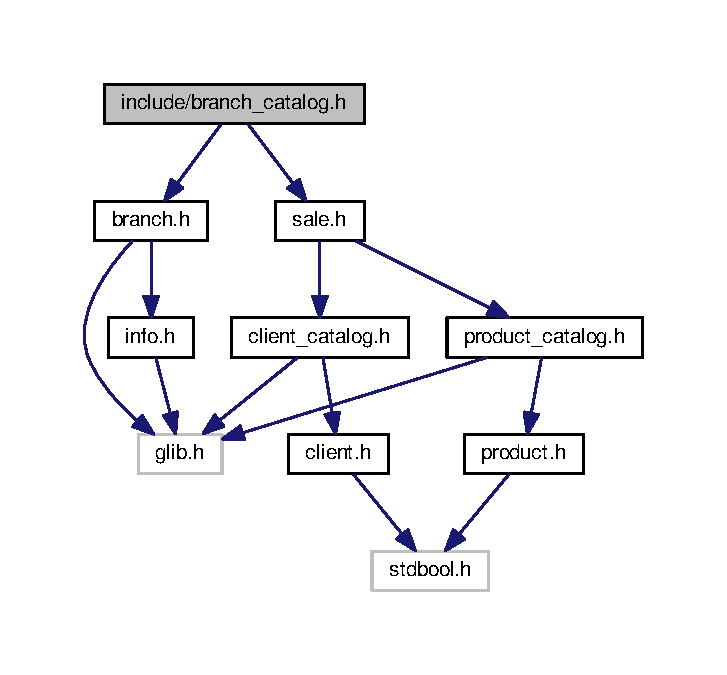
\includegraphics[width=349pt]{branch__catalog_8h__incl}
\end{center}
\end{figure}
\subsection*{Definições de tipos}
\begin{DoxyCompactItemize}
\item 
\mbox{\Hypertarget{branch__catalog_8h_ae69a7625e825eda4ee52d1f1302f68c7}\label{branch__catalog_8h_ae69a7625e825eda4ee52d1f1302f68c7}} 
typedef struct \hyperlink{structbranches}{branches} $\ast$ {\bfseries Branches}
\end{DoxyCompactItemize}
\subsection*{Funções}
\begin{DoxyCompactItemize}
\item 
\hyperlink{structbranches}{Branches} \hyperlink{branch__catalog_8h_a5957cf45168a4c49f0b27592b804f003}{init\+Branches} (int)
\begin{DoxyCompactList}\small\item\em Inicialização da estrutura Branches. \end{DoxyCompactList}\item 
void \hyperlink{branch__catalog_8h_a177c98989c65ec4494a1a01db463efd3}{add\+Branch} (\hyperlink{structbranches}{Branches}, \hyperlink{structbranch}{Branch}, int)
\begin{DoxyCompactList}\small\item\em Adicionar a estrutura Branch á hashtable branches. \end{DoxyCompactList}\item 
void \hyperlink{branch__catalog_8h_a144cb6e992514c3e1059c066f12e3057}{update\+Branches} (\hyperlink{structbranches}{Branches}, \hyperlink{structsale}{Sale})
\begin{DoxyCompactList}\small\item\em Atualizar os dados dentro da estrutura Branches. \end{DoxyCompactList}\item 
void \hyperlink{branch__catalog_8h_a33916718accf07cdbbacf54b4da3afe9}{destroy\+Branches} (\hyperlink{structbranches}{Branches})
\begin{DoxyCompactList}\small\item\em Libertar memória alocada da estrutura Branches. \end{DoxyCompactList}\item 
char $\ast$$\ast$ \hyperlink{branch__catalog_8h_a295f14bacc6ca7e87355e11ac7666701}{clients\+In\+Common} (\hyperlink{structbranches}{Branches}, \hyperlink{structclients}{Clients})
\begin{DoxyCompactList}\small\item\em Encontrar os clientes que compraram em todas as filiais. \end{DoxyCompactList}\item 
char $\ast$$\ast$ \hyperlink{branch__catalog_8h_a3ea8c471feb07ad3ef7b47a61fa65a2b}{get\+Products\+Bought} (\hyperlink{structbranches}{Branches}, int)
\begin{DoxyCompactList}\small\item\em Devolve um array de códigos de produto vendidos numa certa filial. \end{DoxyCompactList}\item 
\hyperlink{structquerie9Aux}{Query9\+Aux} \hyperlink{branch__catalog_8h_a6cbc2ae1db709f8f15375aa2664a3f1f}{clients\+Who\+Bought\+Product} (\hyperlink{structbranches}{Branches}, char $\ast$, int)
\begin{DoxyCompactList}\small\item\em Deolve uma estrutura Query9\+Aux com os valores especificos a um dado código de produto. \end{DoxyCompactList}\item 
char $\ast$$\ast$ \hyperlink{branch__catalog_8h_a54fdf5b5875b1dee2ab8318629d9513a}{get\+Clients\+Used} (\hyperlink{structbranches}{Branches}, int)
\begin{DoxyCompactList}\small\item\em Devolve um array com todos os códigos de cliente de uma certa filial. \end{DoxyCompactList}\item 
int $\ast$ \hyperlink{branch__catalog_8h_aa1dbf339c77602aa2b444dfdc0df22c6}{client\+Branch\+Shop\+Log} (\hyperlink{structbranches}{Branches}, char $\ast$, int)
\begin{DoxyCompactList}\small\item\em Devolve um array com as quantidades de produtos comprados em cada mês. \end{DoxyCompactList}\item 
\hyperlink{structinfo}{Info} $\ast$ \hyperlink{branch__catalog_8h_a095927b2ea100613eb19acca69383ac2}{get\+Most\+Bought} (\hyperlink{structbranches}{Branches}, char $\ast$, int)
\begin{DoxyCompactList}\small\item\em Devolve um array por ordem descendente de por quantidade comprada com a estrutura Info. \end{DoxyCompactList}\item 
\hyperlink{structaux}{Aux} $\ast$ \hyperlink{branch__catalog_8h_ade10d8864b24a178a47892b5f88dae3a}{get\+N\+Most\+Bought\+Products} (\hyperlink{structbranches}{Branches}, int)
\begin{DoxyCompactList}\small\item\em Devolve um array com a estrutura auxiliar Aux com os N produtos mais comprados. \end{DoxyCompactList}\item 
\hyperlink{structmoney}{Money} $\ast$ \hyperlink{branch__catalog_8h_ad4131741611cec37057581c7db43088e}{client\+Spent\+Most\+On} (\hyperlink{structbranches}{Branches}, char $\ast$, int)
\begin{DoxyCompactList}\small\item\em Devolve um array com a estrutura auxiliar Money com os N produtos em que um cliente gastou mais dinheiro. \end{DoxyCompactList}\end{DoxyCompactItemize}


\subsection{Descrição detalhada}
Módulo de tratamentos do catálogo de filiais. 



\subsection{Documentação das funções}
\mbox{\Hypertarget{branch__catalog_8h_a177c98989c65ec4494a1a01db463efd3}\label{branch__catalog_8h_a177c98989c65ec4494a1a01db463efd3}} 
\index{branch\+\_\+catalog.\+h@{branch\+\_\+catalog.\+h}!add\+Branch@{add\+Branch}}
\index{add\+Branch@{add\+Branch}!branch\+\_\+catalog.\+h@{branch\+\_\+catalog.\+h}}
\subsubsection{\texorpdfstring{add\+Branch()}{addBranch()}}
{\footnotesize\ttfamily void add\+Branch (\begin{DoxyParamCaption}\item[{\hyperlink{structbranches}{Branches}}]{,  }\item[{\hyperlink{structbranch}{Branch}}]{,  }\item[{int}]{ }\end{DoxyParamCaption})}



Adicionar a estrutura Branch á hashtable branches. 


\begin{DoxyParams}{Parâmetros}
{\em branches} & Estrutura Branches \\
\hline
{\em branch} & Estrutura Branch a ser inserida \\
\hline
{\em number} & Número da filial que vai ser inserida \\
\hline
\end{DoxyParams}
\mbox{\Hypertarget{branch__catalog_8h_aa1dbf339c77602aa2b444dfdc0df22c6}\label{branch__catalog_8h_aa1dbf339c77602aa2b444dfdc0df22c6}} 
\index{branch\+\_\+catalog.\+h@{branch\+\_\+catalog.\+h}!client\+Branch\+Shop\+Log@{client\+Branch\+Shop\+Log}}
\index{client\+Branch\+Shop\+Log@{client\+Branch\+Shop\+Log}!branch\+\_\+catalog.\+h@{branch\+\_\+catalog.\+h}}
\subsubsection{\texorpdfstring{client\+Branch\+Shop\+Log()}{clientBranchShopLog()}}
{\footnotesize\ttfamily int$\ast$ client\+Branch\+Shop\+Log (\begin{DoxyParamCaption}\item[{\hyperlink{structbranches}{Branches}}]{,  }\item[{char $\ast$}]{,  }\item[{int}]{ }\end{DoxyParamCaption})}



Devolve um array com as quantidades de produtos comprados em cada mês. 


\begin{DoxyParams}{Parâmetros}
{\em bs} & Estrutura Branches \\
\hline
{\em client\+\_\+code} & Código do cliente \\
\hline
{\em branch} & Número da filial escolhida \\
\hline
\end{DoxyParams}
\begin{DoxyReturn}{Retorna}
int$\ast$ Array com quantidades de produtos comprados em cada mês 
\end{DoxyReturn}
\mbox{\Hypertarget{branch__catalog_8h_a295f14bacc6ca7e87355e11ac7666701}\label{branch__catalog_8h_a295f14bacc6ca7e87355e11ac7666701}} 
\index{branch\+\_\+catalog.\+h@{branch\+\_\+catalog.\+h}!clients\+In\+Common@{clients\+In\+Common}}
\index{clients\+In\+Common@{clients\+In\+Common}!branch\+\_\+catalog.\+h@{branch\+\_\+catalog.\+h}}
\subsubsection{\texorpdfstring{clients\+In\+Common()}{clientsInCommon()}}
{\footnotesize\ttfamily char$\ast$$\ast$ clients\+In\+Common (\begin{DoxyParamCaption}\item[{\hyperlink{structbranches}{Branches}}]{,  }\item[{\hyperlink{structclients}{Clients}}]{ }\end{DoxyParamCaption})}



Encontrar os clientes que compraram em todas as filiais. 


\begin{DoxyParams}{Parâmetros}
{\em bs} & Estrutura Branches \\
\hline
{\em clients} & Estrutura Clients \\
\hline
\end{DoxyParams}
\begin{DoxyReturn}{Retorna}
char$\ast$$\ast$ Array de clientes que compraram em todos as filiais 
\end{DoxyReturn}
\mbox{\Hypertarget{branch__catalog_8h_ad4131741611cec37057581c7db43088e}\label{branch__catalog_8h_ad4131741611cec37057581c7db43088e}} 
\index{branch\+\_\+catalog.\+h@{branch\+\_\+catalog.\+h}!client\+Spent\+Most\+On@{client\+Spent\+Most\+On}}
\index{client\+Spent\+Most\+On@{client\+Spent\+Most\+On}!branch\+\_\+catalog.\+h@{branch\+\_\+catalog.\+h}}
\subsubsection{\texorpdfstring{client\+Spent\+Most\+On()}{clientSpentMostOn()}}
{\footnotesize\ttfamily \hyperlink{structmoney}{Money}$\ast$ client\+Spent\+Most\+On (\begin{DoxyParamCaption}\item[{\hyperlink{structbranches}{Branches}}]{,  }\item[{char $\ast$}]{,  }\item[{int}]{ }\end{DoxyParamCaption})}



Devolve um array com a estrutura auxiliar Money com os N produtos em que um cliente gastou mais dinheiro. 


\begin{DoxyParams}{Parâmetros}
{\em bs} & Estrutura Branches \\
\hline
{\em client\+\_\+code} & Código do cliente \\
\hline
{\em n} & Número de produtos a adicionar ao array final \\
\hline
\end{DoxyParams}
\begin{DoxyReturn}{Retorna}
Money$\ast$ Array com estrutura auxiliar para devolver resultados da query 12 
\end{DoxyReturn}
\mbox{\Hypertarget{branch__catalog_8h_a6cbc2ae1db709f8f15375aa2664a3f1f}\label{branch__catalog_8h_a6cbc2ae1db709f8f15375aa2664a3f1f}} 
\index{branch\+\_\+catalog.\+h@{branch\+\_\+catalog.\+h}!clients\+Who\+Bought\+Product@{clients\+Who\+Bought\+Product}}
\index{clients\+Who\+Bought\+Product@{clients\+Who\+Bought\+Product}!branch\+\_\+catalog.\+h@{branch\+\_\+catalog.\+h}}
\subsubsection{\texorpdfstring{clients\+Who\+Bought\+Product()}{clientsWhoBoughtProduct()}}
{\footnotesize\ttfamily \hyperlink{structquerie9Aux}{Query9\+Aux} clients\+Who\+Bought\+Product (\begin{DoxyParamCaption}\item[{\hyperlink{structbranches}{Branches}}]{,  }\item[{char $\ast$}]{,  }\item[{int}]{ }\end{DoxyParamCaption})}



Deolve uma estrutura Query9\+Aux com os valores especificos a um dado código de produto. 


\begin{DoxyParams}{Parâmetros}
{\em bs} & Estrutura Branches \\
\hline
{\em product\+\_\+code} & Código do produto \\
\hline
{\em branch} & Número da filial escolhida \\
\hline
\end{DoxyParams}
\begin{DoxyReturn}{Retorna}
Query9\+Aux Estrutura auxiliar para devolver resultados da query 9 
\end{DoxyReturn}
\mbox{\Hypertarget{branch__catalog_8h_a33916718accf07cdbbacf54b4da3afe9}\label{branch__catalog_8h_a33916718accf07cdbbacf54b4da3afe9}} 
\index{branch\+\_\+catalog.\+h@{branch\+\_\+catalog.\+h}!destroy\+Branches@{destroy\+Branches}}
\index{destroy\+Branches@{destroy\+Branches}!branch\+\_\+catalog.\+h@{branch\+\_\+catalog.\+h}}
\subsubsection{\texorpdfstring{destroy\+Branches()}{destroyBranches()}}
{\footnotesize\ttfamily void destroy\+Branches (\begin{DoxyParamCaption}\item[{\hyperlink{structbranches}{Branches}}]{ }\end{DoxyParamCaption})}



Libertar memória alocada da estrutura Branches. 


\begin{DoxyParams}{Parâmetros}
{\em branches} & Estrutura Branches a ser libertada \\
\hline
\end{DoxyParams}
\mbox{\Hypertarget{branch__catalog_8h_a54fdf5b5875b1dee2ab8318629d9513a}\label{branch__catalog_8h_a54fdf5b5875b1dee2ab8318629d9513a}} 
\index{branch\+\_\+catalog.\+h@{branch\+\_\+catalog.\+h}!get\+Clients\+Used@{get\+Clients\+Used}}
\index{get\+Clients\+Used@{get\+Clients\+Used}!branch\+\_\+catalog.\+h@{branch\+\_\+catalog.\+h}}
\subsubsection{\texorpdfstring{get\+Clients\+Used()}{getClientsUsed()}}
{\footnotesize\ttfamily char$\ast$$\ast$ get\+Clients\+Used (\begin{DoxyParamCaption}\item[{\hyperlink{structbranches}{Branches}}]{,  }\item[{int}]{ }\end{DoxyParamCaption})}



Devolve um array com todos os códigos de cliente de uma certa filial. 


\begin{DoxyParams}{Parâmetros}
{\em bs} & Estrutura Branches \\
\hline
{\em branch} & Número da filial escolhida \\
\hline
\end{DoxyParams}
\begin{DoxyReturn}{Retorna}
char$\ast$$\ast$ Array de códigos de clientes 
\end{DoxyReturn}
\mbox{\Hypertarget{branch__catalog_8h_a095927b2ea100613eb19acca69383ac2}\label{branch__catalog_8h_a095927b2ea100613eb19acca69383ac2}} 
\index{branch\+\_\+catalog.\+h@{branch\+\_\+catalog.\+h}!get\+Most\+Bought@{get\+Most\+Bought}}
\index{get\+Most\+Bought@{get\+Most\+Bought}!branch\+\_\+catalog.\+h@{branch\+\_\+catalog.\+h}}
\subsubsection{\texorpdfstring{get\+Most\+Bought()}{getMostBought()}}
{\footnotesize\ttfamily \hyperlink{structinfo}{Info}$\ast$ get\+Most\+Bought (\begin{DoxyParamCaption}\item[{\hyperlink{structbranches}{Branches}}]{,  }\item[{char $\ast$}]{,  }\item[{int}]{ }\end{DoxyParamCaption})}



Devolve um array por ordem descendente de por quantidade comprada com a estrutura Info. 


\begin{DoxyParams}{Parâmetros}
{\em bs} & Estrutura Branches \\
\hline
{\em client\+\_\+code} & Código do cliente \\
\hline
{\em month} & Mês a procurar \\
\hline
\end{DoxyParams}
\begin{DoxyReturn}{Retorna}
Info Estrutura auxiliar para devolver resultados da query xxx 
\end{DoxyReturn}
\mbox{\Hypertarget{branch__catalog_8h_ade10d8864b24a178a47892b5f88dae3a}\label{branch__catalog_8h_ade10d8864b24a178a47892b5f88dae3a}} 
\index{branch\+\_\+catalog.\+h@{branch\+\_\+catalog.\+h}!get\+N\+Most\+Bought\+Products@{get\+N\+Most\+Bought\+Products}}
\index{get\+N\+Most\+Bought\+Products@{get\+N\+Most\+Bought\+Products}!branch\+\_\+catalog.\+h@{branch\+\_\+catalog.\+h}}
\subsubsection{\texorpdfstring{get\+N\+Most\+Bought\+Products()}{getNMostBoughtProducts()}}
{\footnotesize\ttfamily \hyperlink{structaux}{Aux}$\ast$ get\+N\+Most\+Bought\+Products (\begin{DoxyParamCaption}\item[{\hyperlink{structbranches}{Branches}}]{,  }\item[{int}]{ }\end{DoxyParamCaption})}



Devolve um array com a estrutura auxiliar Aux com os N produtos mais comprados. 


\begin{DoxyParams}{Parâmetros}
{\em bs} & Estrutura Branches \\
\hline
{\em n\+\_\+products} & \\
\hline
\end{DoxyParams}
\begin{DoxyReturn}{Retorna}
Aux Estrutura auxiliar para devolver resultados da query xxx 
\end{DoxyReturn}
\mbox{\Hypertarget{branch__catalog_8h_a3ea8c471feb07ad3ef7b47a61fa65a2b}\label{branch__catalog_8h_a3ea8c471feb07ad3ef7b47a61fa65a2b}} 
\index{branch\+\_\+catalog.\+h@{branch\+\_\+catalog.\+h}!get\+Products\+Bought@{get\+Products\+Bought}}
\index{get\+Products\+Bought@{get\+Products\+Bought}!branch\+\_\+catalog.\+h@{branch\+\_\+catalog.\+h}}
\subsubsection{\texorpdfstring{get\+Products\+Bought()}{getProductsBought()}}
{\footnotesize\ttfamily char$\ast$$\ast$ get\+Products\+Bought (\begin{DoxyParamCaption}\item[{\hyperlink{structbranches}{Branches}}]{,  }\item[{int}]{ }\end{DoxyParamCaption})}



Devolve um array de códigos de produto vendidos numa certa filial. 


\begin{DoxyParams}{Parâmetros}
{\em bs} & Estrutura Branches \\
\hline
{\em branch} & Número da filial escolhida \\
\hline
\end{DoxyParams}
\begin{DoxyReturn}{Retorna}
char$\ast$$\ast$ Array de códigos de produto vendidos numa certa filial 
\end{DoxyReturn}
\mbox{\Hypertarget{branch__catalog_8h_a5957cf45168a4c49f0b27592b804f003}\label{branch__catalog_8h_a5957cf45168a4c49f0b27592b804f003}} 
\index{branch\+\_\+catalog.\+h@{branch\+\_\+catalog.\+h}!init\+Branches@{init\+Branches}}
\index{init\+Branches@{init\+Branches}!branch\+\_\+catalog.\+h@{branch\+\_\+catalog.\+h}}
\subsubsection{\texorpdfstring{init\+Branches()}{initBranches()}}
{\footnotesize\ttfamily \hyperlink{structbranches}{Branches} init\+Branches (\begin{DoxyParamCaption}\item[{int}]{ }\end{DoxyParamCaption})}



Inicialização da estrutura Branches. 


\begin{DoxyParams}{Parâmetros}
{\em branches} & Número de filiais a inicializar \\
\hline
\end{DoxyParams}
\begin{DoxyReturn}{Retorna}
Branches Estrutura Branches inicializada 
\end{DoxyReturn}
\mbox{\Hypertarget{branch__catalog_8h_a144cb6e992514c3e1059c066f12e3057}\label{branch__catalog_8h_a144cb6e992514c3e1059c066f12e3057}} 
\index{branch\+\_\+catalog.\+h@{branch\+\_\+catalog.\+h}!update\+Branches@{update\+Branches}}
\index{update\+Branches@{update\+Branches}!branch\+\_\+catalog.\+h@{branch\+\_\+catalog.\+h}}
\subsubsection{\texorpdfstring{update\+Branches()}{updateBranches()}}
{\footnotesize\ttfamily void update\+Branches (\begin{DoxyParamCaption}\item[{\hyperlink{structbranches}{Branches}}]{,  }\item[{\hyperlink{structsale}{Sale}}]{ }\end{DoxyParamCaption})}



Atualizar os dados dentro da estrutura Branches. 


\begin{DoxyParams}{Parâmetros}
{\em branches} & Estrutura Branches \\
\hline
{\em sale} & Estrutura Sale \\
\hline
\end{DoxyParams}

\hypertarget{client_8h}{}\section{Referência ao ficheiro include/client.h}
\label{client_8h}\index{include/client.\+h@{include/client.\+h}}


Módulo de tratamentos de clientes.  


{\ttfamily \#include $<$stdbool.\+h$>$}\newline
Diagrama de dependências de inclusão para client.\+h\+:
\nopagebreak
\begin{figure}[H]
\begin{center}
\leavevmode
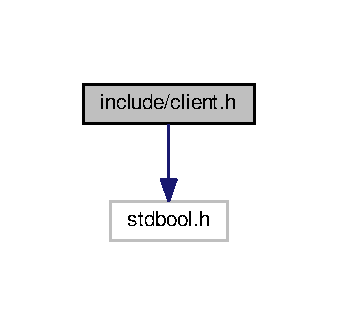
\includegraphics[width=162pt]{client_8h__incl}
\end{center}
\end{figure}
Este grafo mostra quais são os ficheiros que incluem directamente ou indirectamente este ficheiro\+:
\nopagebreak
\begin{figure}[H]
\begin{center}
\leavevmode
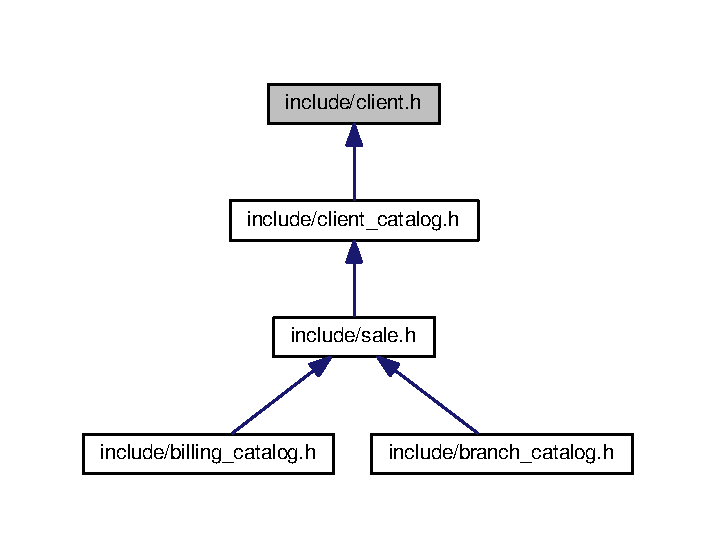
\includegraphics[width=344pt]{client_8h__dep__incl}
\end{center}
\end{figure}
\subsection*{Definições de tipos}
\begin{DoxyCompactItemize}
\item 
\mbox{\Hypertarget{client_8h_a281c2f88dc512deea4afd92a01c223da}\label{client_8h_a281c2f88dc512deea4afd92a01c223da}} 
typedef struct \hyperlink{structclient}{client} $\ast$ {\bfseries Client}
\end{DoxyCompactItemize}
\subsection*{Funções}
\begin{DoxyCompactItemize}
\item 
bool \hyperlink{client_8h_afacce3cde85997aa7b7db2ecd8a1f131}{verify\+Client} (char $\ast$)
\begin{DoxyCompactList}\small\item\em Verifica se um código de cliente é válido. \end{DoxyCompactList}\item 
\hyperlink{structclient}{Client} \hyperlink{client_8h_ad3c48884dd494df3ceda8c679adaa58c}{new\+Client} (char $\ast$)
\begin{DoxyCompactList}\small\item\em Cria um novo Client. \end{DoxyCompactList}\item 
char $\ast$ \hyperlink{client_8h_a42e5defadf41cd4f69dd8978497ec40a}{get\+Client\+Code} (\hyperlink{structclient}{Client})
\begin{DoxyCompactList}\small\item\em Extrai o código de cliente a partir de um Client. \end{DoxyCompactList}\item 
int \hyperlink{client_8h_a417d199a77155f7011ee0c9563b47f60}{equals\+Client} (\hyperlink{structclient}{Client}, \hyperlink{structclient}{Client})
\begin{DoxyCompactList}\small\item\em Compara dois Client. \end{DoxyCompactList}\item 
void \hyperlink{client_8h_a210b336ce5340a6cae03aaf9e7b9e48e}{destroy\+Client} (\hyperlink{structclient}{Client})
\begin{DoxyCompactList}\small\item\em Destroi um Client. \end{DoxyCompactList}\end{DoxyCompactItemize}


\subsection{Descrição detalhada}
Módulo de tratamentos de clientes. 



\subsection{Documentação das funções}
\mbox{\Hypertarget{client_8h_a210b336ce5340a6cae03aaf9e7b9e48e}\label{client_8h_a210b336ce5340a6cae03aaf9e7b9e48e}} 
\index{client.\+h@{client.\+h}!destroy\+Client@{destroy\+Client}}
\index{destroy\+Client@{destroy\+Client}!client.\+h@{client.\+h}}
\subsubsection{\texorpdfstring{destroy\+Client()}{destroyClient()}}
{\footnotesize\ttfamily void destroy\+Client (\begin{DoxyParamCaption}\item[{\hyperlink{structclient}{Client}}]{ }\end{DoxyParamCaption})}



Destroi um Client. 


\begin{DoxyParams}{Parâmetros}
{\em client} & Cliente a ser destruido \\
\hline
\end{DoxyParams}
\mbox{\Hypertarget{client_8h_a417d199a77155f7011ee0c9563b47f60}\label{client_8h_a417d199a77155f7011ee0c9563b47f60}} 
\index{client.\+h@{client.\+h}!equals\+Client@{equals\+Client}}
\index{equals\+Client@{equals\+Client}!client.\+h@{client.\+h}}
\subsubsection{\texorpdfstring{equals\+Client()}{equalsClient()}}
{\footnotesize\ttfamily int equals\+Client (\begin{DoxyParamCaption}\item[{\hyperlink{structclient}{Client}}]{,  }\item[{\hyperlink{structclient}{Client}}]{ }\end{DoxyParamCaption})}



Compara dois Client. 


\begin{DoxyParams}{Parâmetros}
{\em a} & Primeiro cliente \\
\hline
{\em b} & Segundo cliente \\
\hline
\end{DoxyParams}
\begin{DoxyReturn}{Retorna}
int Resultado da comparação 
\end{DoxyReturn}
\mbox{\Hypertarget{client_8h_a42e5defadf41cd4f69dd8978497ec40a}\label{client_8h_a42e5defadf41cd4f69dd8978497ec40a}} 
\index{client.\+h@{client.\+h}!get\+Client\+Code@{get\+Client\+Code}}
\index{get\+Client\+Code@{get\+Client\+Code}!client.\+h@{client.\+h}}
\subsubsection{\texorpdfstring{get\+Client\+Code()}{getClientCode()}}
{\footnotesize\ttfamily char$\ast$ get\+Client\+Code (\begin{DoxyParamCaption}\item[{\hyperlink{structclient}{Client}}]{ }\end{DoxyParamCaption})}



Extrai o código de cliente a partir de um Client. 


\begin{DoxyParams}{Parâmetros}
{\em client} & Client que contém as informações do cliente \\
\hline
\end{DoxyParams}
\begin{DoxyReturn}{Retorna}
char$\ast$ Código de cliente 
\end{DoxyReturn}
\mbox{\Hypertarget{client_8h_ad3c48884dd494df3ceda8c679adaa58c}\label{client_8h_ad3c48884dd494df3ceda8c679adaa58c}} 
\index{client.\+h@{client.\+h}!new\+Client@{new\+Client}}
\index{new\+Client@{new\+Client}!client.\+h@{client.\+h}}
\subsubsection{\texorpdfstring{new\+Client()}{newClient()}}
{\footnotesize\ttfamily \hyperlink{structclient}{Client} new\+Client (\begin{DoxyParamCaption}\item[{char $\ast$}]{ }\end{DoxyParamCaption})}



Cria um novo Client. 


\begin{DoxyParams}{Parâmetros}
{\em client} & Código de cliente \\
\hline
\end{DoxyParams}
\begin{DoxyReturn}{Retorna}
Client Client criado a partir do código 
\end{DoxyReturn}
\mbox{\Hypertarget{client_8h_afacce3cde85997aa7b7db2ecd8a1f131}\label{client_8h_afacce3cde85997aa7b7db2ecd8a1f131}} 
\index{client.\+h@{client.\+h}!verify\+Client@{verify\+Client}}
\index{verify\+Client@{verify\+Client}!client.\+h@{client.\+h}}
\subsubsection{\texorpdfstring{verify\+Client()}{verifyClient()}}
{\footnotesize\ttfamily bool verify\+Client (\begin{DoxyParamCaption}\item[{char $\ast$}]{ }\end{DoxyParamCaption})}



Verifica se um código de cliente é válido. 


\begin{DoxyParams}{Parâmetros}
{\em client} & Código de cliente \\
\hline
\end{DoxyParams}
\begin{DoxyReturn}{Retorna}
bool Verificação se o código de cliente é válido ou não 
\end{DoxyReturn}

\hypertarget{client__catalog_8h}{}\section{Referência ao ficheiro include/client\+\_\+catalog.h}
\label{client__catalog_8h}\index{include/client\+\_\+catalog.\+h@{include/client\+\_\+catalog.\+h}}


Módulo de tratamentos do catálogo de clientes.  


{\ttfamily \#include \char`\"{}client.\+h\char`\"{}}\newline
{\ttfamily \#include $<$glib.\+h$>$}\newline
Diagrama de dependências de inclusão para client\+\_\+catalog.\+h\+:
\nopagebreak
\begin{figure}[H]
\begin{center}
\leavevmode
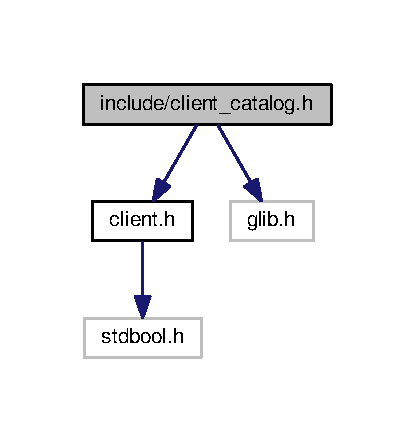
\includegraphics[width=199pt]{client__catalog_8h__incl}
\end{center}
\end{figure}
Este grafo mostra quais são os ficheiros que incluem directamente ou indirectamente este ficheiro\+:
\nopagebreak
\begin{figure}[H]
\begin{center}
\leavevmode
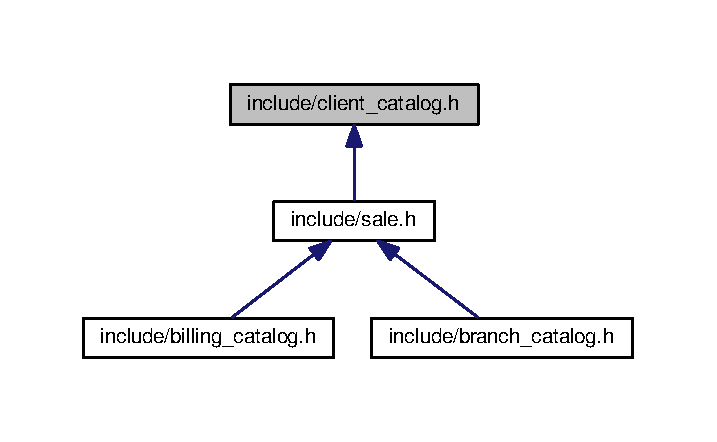
\includegraphics[width=344pt]{client__catalog_8h__dep__incl}
\end{center}
\end{figure}
\subsection*{Definições de tipos}
\begin{DoxyCompactItemize}
\item 
\mbox{\Hypertarget{client__catalog_8h_a3df8b5aa1e44995afa1727417dcedd4e}\label{client__catalog_8h_a3df8b5aa1e44995afa1727417dcedd4e}} 
typedef struct \hyperlink{structclients}{clients} $\ast$ {\bfseries Clients}
\end{DoxyCompactItemize}
\subsection*{Funções}
\begin{DoxyCompactItemize}
\item 
\hyperlink{structclients}{Clients} \hyperlink{client__catalog_8h_a7031e24c518cc5e26729c2badb53947a}{init\+Clients} ()
\begin{DoxyCompactList}\small\item\em Inicia a estrutura de catálogo de clientes. \end{DoxyCompactList}\item 
int \hyperlink{client__catalog_8h_a66fdcc00fe6adc95ab8402bb32b9ea7e}{add\+Client} (\hyperlink{structclients}{Clients}, char $\ast$)
\begin{DoxyCompactList}\small\item\em Adiciona um cliente ao catálogo de clientes. \end{DoxyCompactList}\item 
int \hyperlink{client__catalog_8h_ab2dda1e1d6b3dd21bf6605a94b6ea4c8}{get\+Size\+Clients} (\hyperlink{structclients}{Clients})
\begin{DoxyCompactList}\small\item\em Calcula o número de clientes que existe no catálogo. \end{DoxyCompactList}\item 
int \hyperlink{client__catalog_8h_aeb90992c20b0a666f7e098ac98265a37}{exist\+Client} (\hyperlink{structclients}{Clients}, \hyperlink{structclient}{Client})
\begin{DoxyCompactList}\small\item\em Verifica se existe um cliente no catálogo. \end{DoxyCompactList}\item 
int \hyperlink{client__catalog_8h_a33694f5c5e1bfb22ca890b5b3f93de01}{exist\+Client\+Code} (\hyperlink{structclients}{Clients}, char $\ast$)
\begin{DoxyCompactList}\small\item\em Verifica se existe um código de cliente no catálogo. \end{DoxyCompactList}\item 
void \hyperlink{client__catalog_8h_a9ef396154e90aeb16a8bc483d43934e8}{destroy\+Clients} (\hyperlink{structclients}{Clients})
\begin{DoxyCompactList}\small\item\em Destroi o catálogo de clientes. \end{DoxyCompactList}\item 
int \hyperlink{client__catalog_8h_ad7634a72484814b664df73c2d113f67a}{get\+Number\+Clients\+Not\+Used} (\hyperlink{structclients}{Clients}, G\+Hash\+Table $\ast$)
\begin{DoxyCompactList}\small\item\em Devolve o número de clientes não utilizados. \end{DoxyCompactList}\item 
void \hyperlink{client__catalog_8h_a64e9647162e8138dcefd16b8eb6ef802}{fill\+Clients\+HT} (\hyperlink{structclients}{Clients}, G\+Hash\+Table $\ast$)
\begin{DoxyCompactList}\small\item\em Preencher a hashtable dada com todos os códigos de clientes. \end{DoxyCompactList}\end{DoxyCompactItemize}


\subsection{Descrição detalhada}
Módulo de tratamentos do catálogo de clientes. 



\subsection{Documentação das funções}
\mbox{\Hypertarget{client__catalog_8h_a66fdcc00fe6adc95ab8402bb32b9ea7e}\label{client__catalog_8h_a66fdcc00fe6adc95ab8402bb32b9ea7e}} 
\index{client\+\_\+catalog.\+h@{client\+\_\+catalog.\+h}!add\+Client@{add\+Client}}
\index{add\+Client@{add\+Client}!client\+\_\+catalog.\+h@{client\+\_\+catalog.\+h}}
\subsubsection{\texorpdfstring{add\+Client()}{addClient()}}
{\footnotesize\ttfamily int add\+Client (\begin{DoxyParamCaption}\item[{\hyperlink{structclients}{Clients}}]{,  }\item[{char $\ast$}]{ }\end{DoxyParamCaption})}



Adiciona um cliente ao catálogo de clientes. 


\begin{DoxyParams}{Parâmetros}
{\em clients} & Catálogo de clientes ao qual vai ser adicionado o novo cliente \\
\hline
{\em client} & Cliente a ser adicionado ao catálogo de clientes \\
\hline
\end{DoxyParams}
\begin{DoxyReturn}{Retorna}
int Verificação da inserção 
\end{DoxyReturn}
\mbox{\Hypertarget{client__catalog_8h_a9ef396154e90aeb16a8bc483d43934e8}\label{client__catalog_8h_a9ef396154e90aeb16a8bc483d43934e8}} 
\index{client\+\_\+catalog.\+h@{client\+\_\+catalog.\+h}!destroy\+Clients@{destroy\+Clients}}
\index{destroy\+Clients@{destroy\+Clients}!client\+\_\+catalog.\+h@{client\+\_\+catalog.\+h}}
\subsubsection{\texorpdfstring{destroy\+Clients()}{destroyClients()}}
{\footnotesize\ttfamily void destroy\+Clients (\begin{DoxyParamCaption}\item[{\hyperlink{structclients}{Clients}}]{ }\end{DoxyParamCaption})}



Destroi o catálogo de clientes. 


\begin{DoxyParams}{Parâmetros}
{\em clients} & Catálogo de clientes \\
\hline
\end{DoxyParams}
\mbox{\Hypertarget{client__catalog_8h_aeb90992c20b0a666f7e098ac98265a37}\label{client__catalog_8h_aeb90992c20b0a666f7e098ac98265a37}} 
\index{client\+\_\+catalog.\+h@{client\+\_\+catalog.\+h}!exist\+Client@{exist\+Client}}
\index{exist\+Client@{exist\+Client}!client\+\_\+catalog.\+h@{client\+\_\+catalog.\+h}}
\subsubsection{\texorpdfstring{exist\+Client()}{existClient()}}
{\footnotesize\ttfamily int exist\+Client (\begin{DoxyParamCaption}\item[{\hyperlink{structclients}{Clients}}]{,  }\item[{\hyperlink{structclient}{Client}}]{ }\end{DoxyParamCaption})}



Verifica se existe um cliente no catálogo. 


\begin{DoxyParams}{Parâmetros}
{\em clients} & Catálogo de clientes \\
\hline
{\em client} & Cliente a ser consultado \\
\hline
\end{DoxyParams}
\begin{DoxyReturn}{Retorna}
int Verificação da procura 
\end{DoxyReturn}
\mbox{\Hypertarget{client__catalog_8h_a33694f5c5e1bfb22ca890b5b3f93de01}\label{client__catalog_8h_a33694f5c5e1bfb22ca890b5b3f93de01}} 
\index{client\+\_\+catalog.\+h@{client\+\_\+catalog.\+h}!exist\+Client\+Code@{exist\+Client\+Code}}
\index{exist\+Client\+Code@{exist\+Client\+Code}!client\+\_\+catalog.\+h@{client\+\_\+catalog.\+h}}
\subsubsection{\texorpdfstring{exist\+Client\+Code()}{existClientCode()}}
{\footnotesize\ttfamily int exist\+Client\+Code (\begin{DoxyParamCaption}\item[{\hyperlink{structclients}{Clients}}]{,  }\item[{char $\ast$}]{ }\end{DoxyParamCaption})}



Verifica se existe um código de cliente no catálogo. 


\begin{DoxyParams}{Parâmetros}
{\em clients} & Catálogo de clientes \\
\hline
{\em client\+\_\+code} & Código de cliente \\
\hline
\end{DoxyParams}
\begin{DoxyReturn}{Retorna}
int Verificação da procura 
\end{DoxyReturn}
\mbox{\Hypertarget{client__catalog_8h_a64e9647162e8138dcefd16b8eb6ef802}\label{client__catalog_8h_a64e9647162e8138dcefd16b8eb6ef802}} 
\index{client\+\_\+catalog.\+h@{client\+\_\+catalog.\+h}!fill\+Clients\+HT@{fill\+Clients\+HT}}
\index{fill\+Clients\+HT@{fill\+Clients\+HT}!client\+\_\+catalog.\+h@{client\+\_\+catalog.\+h}}
\subsubsection{\texorpdfstring{fill\+Clients\+H\+T()}{fillClientsHT()}}
{\footnotesize\ttfamily void fill\+Clients\+HT (\begin{DoxyParamCaption}\item[{\hyperlink{structclients}{Clients}}]{,  }\item[{G\+Hash\+Table $\ast$}]{ }\end{DoxyParamCaption})}



Preencher a hashtable dada com todos os códigos de clientes. 


\begin{DoxyParams}{Parâmetros}
{\em clients} & Estrutura de clientes \\
\hline
{\em clients\+\_\+ht} & Hashtable a ser preenchida \\
\hline
\end{DoxyParams}
\mbox{\Hypertarget{client__catalog_8h_ad7634a72484814b664df73c2d113f67a}\label{client__catalog_8h_ad7634a72484814b664df73c2d113f67a}} 
\index{client\+\_\+catalog.\+h@{client\+\_\+catalog.\+h}!get\+Number\+Clients\+Not\+Used@{get\+Number\+Clients\+Not\+Used}}
\index{get\+Number\+Clients\+Not\+Used@{get\+Number\+Clients\+Not\+Used}!client\+\_\+catalog.\+h@{client\+\_\+catalog.\+h}}
\subsubsection{\texorpdfstring{get\+Number\+Clients\+Not\+Used()}{getNumberClientsNotUsed()}}
{\footnotesize\ttfamily int get\+Number\+Clients\+Not\+Used (\begin{DoxyParamCaption}\item[{\hyperlink{structclients}{Clients}}]{,  }\item[{G\+Hash\+Table $\ast$}]{ }\end{DoxyParamCaption})}



Devolve o número de clientes não utilizados. 


\begin{DoxyParams}{Parâmetros}
{\em client\+\_\+catalog} & Estrutura de clientes \\
\hline
{\em clients\+\_\+used} & Hashtable com os códigos de clientes usados \\
\hline
\end{DoxyParams}
\begin{DoxyReturn}{Retorna}
int Número de clientes não usados 
\end{DoxyReturn}
\mbox{\Hypertarget{client__catalog_8h_ab2dda1e1d6b3dd21bf6605a94b6ea4c8}\label{client__catalog_8h_ab2dda1e1d6b3dd21bf6605a94b6ea4c8}} 
\index{client\+\_\+catalog.\+h@{client\+\_\+catalog.\+h}!get\+Size\+Clients@{get\+Size\+Clients}}
\index{get\+Size\+Clients@{get\+Size\+Clients}!client\+\_\+catalog.\+h@{client\+\_\+catalog.\+h}}
\subsubsection{\texorpdfstring{get\+Size\+Clients()}{getSizeClients()}}
{\footnotesize\ttfamily int get\+Size\+Clients (\begin{DoxyParamCaption}\item[{\hyperlink{structclients}{Clients}}]{ }\end{DoxyParamCaption})}



Calcula o número de clientes que existe no catálogo. 


\begin{DoxyParams}{Parâmetros}
{\em clients} & Catálogo de clientes \\
\hline
\end{DoxyParams}
\begin{DoxyReturn}{Retorna}
int Número de clientes existentes no catálogo 
\end{DoxyReturn}
\mbox{\Hypertarget{client__catalog_8h_a7031e24c518cc5e26729c2badb53947a}\label{client__catalog_8h_a7031e24c518cc5e26729c2badb53947a}} 
\index{client\+\_\+catalog.\+h@{client\+\_\+catalog.\+h}!init\+Clients@{init\+Clients}}
\index{init\+Clients@{init\+Clients}!client\+\_\+catalog.\+h@{client\+\_\+catalog.\+h}}
\subsubsection{\texorpdfstring{init\+Clients()}{initClients()}}
{\footnotesize\ttfamily \hyperlink{structclients}{Clients} init\+Clients (\begin{DoxyParamCaption}{ }\end{DoxyParamCaption})}



Inicia a estrutura de catálogo de clientes. 

\begin{DoxyReturn}{Retorna}
Clients estrutura inicializada 
\end{DoxyReturn}

\hypertarget{controller_8h}{}\section{Referência ao ficheiro include/controller.h}
\label{controller_8h}\index{include/controller.\+h@{include/controller.\+h}}


Módulo do controller.  


Este grafo mostra quais são os ficheiros que incluem directamente ou indirectamente este ficheiro\+:
\nopagebreak
\begin{figure}[H]
\begin{center}
\leavevmode
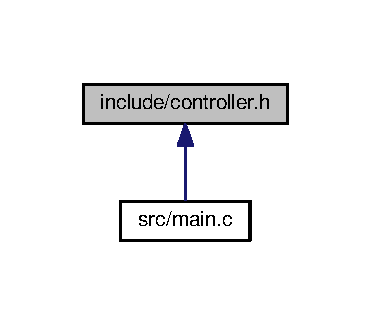
\includegraphics[width=178pt]{controller_8h__dep__incl}
\end{center}
\end{figure}
\subsection*{Funções}
\begin{DoxyCompactItemize}
\item 
\mbox{\Hypertarget{controller_8h_abb8952a2256ad4fa28a72549bd3e56fb}\label{controller_8h_abb8952a2256ad4fa28a72549bd3e56fb}} 
void \hyperlink{controller_8h_abb8952a2256ad4fa28a72549bd3e56fb}{start\+Controller} ()
\begin{DoxyCompactList}\small\item\em Inicializa o controller. \end{DoxyCompactList}\end{DoxyCompactItemize}


\subsection{Descrição detalhada}
Módulo do controller. 


\hypertarget{glibW_8h}{}\section{Referência ao ficheiro include/glibW.h}
\label{glibW_8h}\index{include/glib\+W.\+h@{include/glib\+W.\+h}}


Módulo de tratamento do carregamento da glib.  


{\ttfamily \#include $<$glib.\+h$>$}\newline
Diagrama de dependências de inclusão para glib\+W.\+h\+:
\nopagebreak
\begin{figure}[H]
\begin{center}
\leavevmode
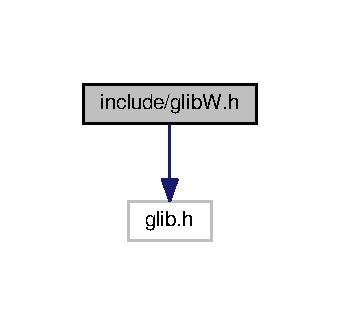
\includegraphics[width=163pt]{glibW_8h__incl}
\end{center}
\end{figure}


\subsection{Descrição detalhada}
Módulo de tratamento do carregamento da glib. 


\hypertarget{info_8h}{}\section{Referência ao ficheiro include/info.h}
\label{info_8h}\index{include/info.\+h@{include/info.\+h}}


Módulo de estruturas auxiliares.  


{\ttfamily \#include $<$glib.\+h$>$}\newline
Diagrama de dependências de inclusão para info.\+h\+:
\nopagebreak
\begin{figure}[H]
\begin{center}
\leavevmode
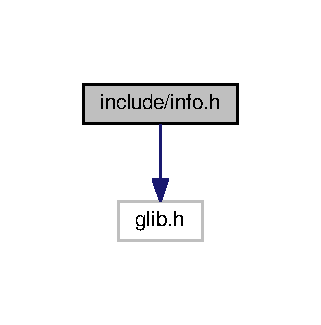
\includegraphics[width=154pt]{info_8h__incl}
\end{center}
\end{figure}
Este grafo mostra quais são os ficheiros que incluem directamente ou indirectamente este ficheiro\+:
\nopagebreak
\begin{figure}[H]
\begin{center}
\leavevmode
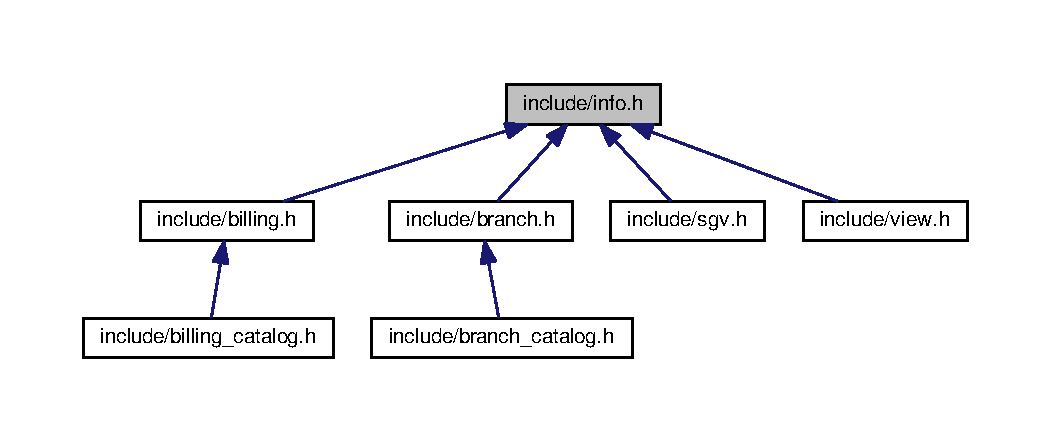
\includegraphics[width=350pt]{info_8h__dep__incl}
\end{center}
\end{figure}
\subsection*{Definições de tipos}
\begin{DoxyCompactItemize}
\item 
\mbox{\Hypertarget{info_8h_ace3735d4dbcdbbfd41af7e66c2109f66}\label{info_8h_ace3735d4dbcdbbfd41af7e66c2109f66}} 
typedef struct \hyperlink{structinfo}{info} $\ast$ {\bfseries Info}
\item 
\mbox{\Hypertarget{info_8h_a8cb5bb662bdd321685bbea94850b6d93}\label{info_8h_a8cb5bb662bdd321685bbea94850b6d93}} 
typedef struct \hyperlink{structaux}{aux} $\ast$ {\bfseries Aux}
\item 
\mbox{\Hypertarget{info_8h_a5be42c2aa391342562cfb37cca5adf2d}\label{info_8h_a5be42c2aa391342562cfb37cca5adf2d}} 
typedef struct \hyperlink{structmoney}{money} $\ast$ {\bfseries Money}
\item 
\mbox{\Hypertarget{info_8h_a5b12898a31f33f8a1c50649159917f5a}\label{info_8h_a5b12898a31f33f8a1c50649159917f5a}} 
typedef struct \hyperlink{structquerie8Aux}{querie8\+Aux} $\ast$ {\bfseries Query8\+Aux}
\item 
\mbox{\Hypertarget{info_8h_afc46fe447d765ea30120d60561f534d7}\label{info_8h_afc46fe447d765ea30120d60561f534d7}} 
typedef struct \hyperlink{structquerie9Aux}{querie9\+Aux} $\ast$ {\bfseries Query9\+Aux}
\end{DoxyCompactItemize}
\subsection*{Funções}
\begin{DoxyCompactItemize}
\item 
int \hyperlink{info_8h_ae6a87f3d83667e1bf1c790f10a859c75}{compare\+Money} (gconstpointer, gconstpointer)
\begin{DoxyCompactList}\small\item\em Compara duas variáveis das estruturas Money. \end{DoxyCompactList}\item 
\hyperlink{structmoney}{Money} \hyperlink{info_8h_a9897ebca004309ef0519361767d65d73}{clone\+Money} (\hyperlink{structmoney}{Money})
\begin{DoxyCompactList}\small\item\em Copia as informações para uma nova estrutura Money. \end{DoxyCompactList}\item 
void \hyperlink{info_8h_a5bcb355ab224d310644f929d6ff81d74}{free\+Money} (\hyperlink{structmoney}{Money})
\begin{DoxyCompactList}\small\item\em Libertação da estrutura Money. \end{DoxyCompactList}\item 
\hyperlink{structaux}{Aux} \hyperlink{info_8h_a0d19488de5aa32654560272982370eec}{clone\+Aux} (\hyperlink{structaux}{Aux})
\begin{DoxyCompactList}\small\item\em Copia as informações para uma nova estrutura Aux. \end{DoxyCompactList}\item 
void \hyperlink{info_8h_aa8e191d81b99db54f59d7af7855c4543}{free\+Aux} (\hyperlink{structaux}{Aux})
\begin{DoxyCompactList}\small\item\em Libertação da estrutura Aux. \end{DoxyCompactList}\item 
int \hyperlink{info_8h_a7c4636f23d9c07e3b0d7388f278732e8}{compare\+Aux} (gconstpointer, gconstpointer)
\begin{DoxyCompactList}\small\item\em Compara duas variáveis das estruturas Aux. \end{DoxyCompactList}\item 
int \hyperlink{info_8h_a2b5b09e1cd11423a2c95a8bf3110db75}{compare\+Info} (gconstpointer, gconstpointer)
\begin{DoxyCompactList}\small\item\em Compara duas variáveis das estruturas Info. \end{DoxyCompactList}\item 
\hyperlink{structinfo}{Info} \hyperlink{info_8h_af1a12e5c8b8198f71c4142a1ea0e2f47}{clone\+Info} (\hyperlink{structinfo}{Info})
\begin{DoxyCompactList}\small\item\em Copia as informações para uma nova estrutura Info. \end{DoxyCompactList}\item 
void \hyperlink{info_8h_a02f55228347268f56c75ffee9d391f75}{free\+Info} (\hyperlink{structinfo}{Info})
\begin{DoxyCompactList}\small\item\em Libertação da estrutura Info. \end{DoxyCompactList}\item 
\hyperlink{structmoney}{Money} \hyperlink{info_8h_a3e93b1821285cb2d28ab911eef26c042}{init\+Money} (char $\ast$, double)
\begin{DoxyCompactList}\small\item\em Inicialização da estrutura Money. \end{DoxyCompactList}\item 
void \hyperlink{info_8h_a8dcbb1118baaf5c859856ad253a2fc19}{update\+Money} (\hyperlink{structmoney}{Money}, double)
\begin{DoxyCompactList}\small\item\em Atualizar os dados dentro da estrutura Money. \end{DoxyCompactList}\item 
void \hyperlink{info_8h_a09807876a097ecacaa4a11e33c163912}{update\+Aux} (\hyperlink{structaux}{Aux}, int, int $\ast$)
\begin{DoxyCompactList}\small\item\em Atualizar os dados dentro da estrutura Aux. \end{DoxyCompactList}\item 
\hyperlink{structaux}{Aux} \hyperlink{info_8h_a4ffac6ae942e26044175ed3685a9ee06}{init\+Aux} (char $\ast$, int, int $\ast$)
\begin{DoxyCompactList}\small\item\em Inicialização da estrutura Aux. \end{DoxyCompactList}\item 
void \hyperlink{info_8h_a2a6c333c5b65eb17a09aa84264883fee}{update\+Info} (\hyperlink{structinfo}{Info}, int)
\begin{DoxyCompactList}\small\item\em Atualizar os dados dentro da estrutura Info. \end{DoxyCompactList}\item 
\hyperlink{structinfo}{Info} \hyperlink{info_8h_aaa28f2db07c8646493aa26a239fc84e2}{init\+Info} (char $\ast$, int)
\begin{DoxyCompactList}\small\item\em Inicialização da estrutura Info. \end{DoxyCompactList}\item 
void \hyperlink{info_8h_a91c45adcbadb92117ef75f5ae03ed9b3}{free\+Info\+List} (\hyperlink{structinfo}{Info} $\ast$)
\begin{DoxyCompactList}\small\item\em Libertação de um array de estruturas Info. \end{DoxyCompactList}\item 
void \hyperlink{info_8h_a3cfad62e6dd3e5e4a3e6420ceb76b07f}{free\+Aux\+List} (\hyperlink{structaux}{Aux} $\ast$)
\begin{DoxyCompactList}\small\item\em Libertação de um array de estruturas Aux. \end{DoxyCompactList}\item 
void \hyperlink{info_8h_a38f2c11521b19fe8e511538fa93895e2}{free\+Money\+List} (\hyperlink{structmoney}{Money} $\ast$)
\begin{DoxyCompactList}\small\item\em Libertação de um array de estruturas Money. \end{DoxyCompactList}\item 
char $\ast$ \hyperlink{info_8h_a86117d019d643bf4cf2f77adb54d6424}{get\+Info\+Product} (\hyperlink{structinfo}{Info})
\begin{DoxyCompactList}\small\item\em Devolve o código de produto da estrutura Info. \end{DoxyCompactList}\item 
char $\ast$ \hyperlink{info_8h_ae50a03e328a6219dcafffdeed6612e03}{get\+Aux\+Product} (\hyperlink{structaux}{Aux})
\begin{DoxyCompactList}\small\item\em Devolve o código de produto da estrutura Aux. \end{DoxyCompactList}\item 
int \hyperlink{info_8h_aa86691fb5fd4dfadcb448ebf08f88bf0}{get\+Aux\+Units\+Sold} (\hyperlink{structaux}{Aux}, int)
\begin{DoxyCompactList}\small\item\em Devolve as unidades vendidas num certo mês presente na estrutura Aux. \end{DoxyCompactList}\item 
int \hyperlink{info_8h_aceb4ce880195ac25ef9ae7c098540769}{get\+Aux\+Total\+Clients} (\hyperlink{structaux}{Aux}, int)
\begin{DoxyCompactList}\small\item\em Devolve o número de clientes num certo mês presente na estrutura Aux. \end{DoxyCompactList}\item 
char $\ast$ \hyperlink{info_8h_a138aa8cf2154669ef15e84ce74e06d45}{get\+Money\+Product} (\hyperlink{structmoney}{Money})
\begin{DoxyCompactList}\small\item\em Devolve o código de produto da estrutura Money. \end{DoxyCompactList}\item 
double \hyperlink{info_8h_aa5fdab4904f6904db621cfc72c2e1396}{get\+Money\+Spent} (\hyperlink{structmoney}{Money} \hyperlink{structmoney}{money})
\begin{DoxyCompactList}\small\item\em Devolve o montante gasto da estrutura Money. \end{DoxyCompactList}\item 
int \hyperlink{info_8h_a32f82a70c5c768ad53d9ee949e923978}{get\+Info\+Units\+Sold} (\hyperlink{structinfo}{Info} \hyperlink{structinfo}{info})
\begin{DoxyCompactList}\small\item\em Devolve a quantidade de unidades vendidas da estrutura Info. \end{DoxyCompactList}\item 
void \hyperlink{info_8h_a5e2a7d6ef4d5c08feeef9b223c5c7523}{update\+Querie8} (\hyperlink{structquerie8Aux}{Query8\+Aux}, double, int, int)
\begin{DoxyCompactList}\small\item\em Atualizar os dados dentro da estrutura Query8\+Aux. \end{DoxyCompactList}\item 
\hyperlink{structquerie8Aux}{Query8\+Aux} \hyperlink{info_8h_acbb9ebb2e64172f022495d4315a62b5f}{init\+Query8\+Aux} ()
\begin{DoxyCompactList}\small\item\em Inicialização da estrutura Query8\+Aux. \end{DoxyCompactList}\item 
int \hyperlink{info_8h_aee9b579abe8647c7277bbdf8f1659a78}{get\+Query8\+Aux\+Units} (\hyperlink{structquerie8Aux}{Query8\+Aux})
\begin{DoxyCompactList}\small\item\em Devolve a quantidade de unidades vendidas da estrutura Aux. \end{DoxyCompactList}\item 
double \hyperlink{info_8h_ad8a318effd5a52c4c17eec7a93bc414b}{get\+Query8\+Aux\+Billed} (\hyperlink{structquerie8Aux}{Query8\+Aux})
\begin{DoxyCompactList}\small\item\em Devolve o total faturado da estrutura Aux. \end{DoxyCompactList}\item 
int \hyperlink{info_8h_a586f4db6ee04b0812b97c24d2ec35179}{get\+Query8\+Aux\+Sales} (\hyperlink{structquerie8Aux}{Query8\+Aux})
\begin{DoxyCompactList}\small\item\em Devolve a quantidade de vendas da estrutura Aux. \end{DoxyCompactList}\item 
void \hyperlink{info_8h_a0db65b71e143a903ca2224ed70f479fe}{free\+Query8\+Aux} (\hyperlink{structquerie8Aux}{Query8\+Aux})
\begin{DoxyCompactList}\small\item\em Libertação da estrutura Query8\+Aux. \end{DoxyCompactList}\item 
void \hyperlink{info_8h_affe2daef7c78e1f350333228f4fd4de9}{update\+TotalN} (\hyperlink{structquerie9Aux}{Query9\+Aux})
\begin{DoxyCompactList}\small\item\em Incrementa o valor totalN dentro da estrutura Query9\+Aux. \end{DoxyCompactList}\item 
void \hyperlink{info_8h_a61d62b83860d662dad2c66726492ac80}{update\+TotalP} (\hyperlink{structquerie9Aux}{Query9\+Aux})
\begin{DoxyCompactList}\small\item\em Incrementa o valor totalP dentro da estrutura Queries9\+Aux. \end{DoxyCompactList}\item 
int \hyperlink{info_8h_abdbe946638abb7ee3fd23e8a1a086978}{get\+Query9\+TotalN} (\hyperlink{structquerie9Aux}{Query9\+Aux} \hyperlink{structaux}{aux})
\begin{DoxyCompactList}\small\item\em Devolve o valor de totalN da estrutura Query9\+Aux. \end{DoxyCompactList}\item 
int \hyperlink{info_8h_a2f31b1f7ceeae58539b1bf0c9e0c58b9}{get\+Query9\+TotalP} (\hyperlink{structquerie9Aux}{Query9\+Aux} \hyperlink{structaux}{aux})
\begin{DoxyCompactList}\small\item\em Devolve o valor de totalP da estrutura Query9\+Aux. \end{DoxyCompactList}\item 
\hyperlink{structquerie9Aux}{Query9\+Aux} \hyperlink{info_8h_aea18480202920b30bcd9d16900a23c85}{init\+Query9\+Aux} (int)
\begin{DoxyCompactList}\small\item\em Inicialização da estrutura Query9\+Aux. \end{DoxyCompactList}\item 
void \hyperlink{info_8h_a9f4fc43ae49040fb52aad9e1b5617b87}{update\+ClientsN} (\hyperlink{structquerie9Aux}{Query9\+Aux}, int, char $\ast$)
\begin{DoxyCompactList}\small\item\em Atualizar o valor clientsN de um certo índice na estrutura Query9\+Aux. \end{DoxyCompactList}\item 
void \hyperlink{info_8h_a134b3e65ffa192be4fe79cd820701e69}{update\+ClientsP} (\hyperlink{structquerie9Aux}{Query9\+Aux}, int, char $\ast$)
\begin{DoxyCompactList}\small\item\em Atualizar o valor clientsP de um certo índice na estrutura Query9\+Aux. \end{DoxyCompactList}\item 
void \hyperlink{info_8h_a07ef3e30aadd27d5c2ec8527b6d3f007}{update\+Clients} (\hyperlink{structquerie9Aux}{Query9\+Aux}, int, int)
\begin{DoxyCompactList}\small\item\em Atualizar clientsN e clientsP para N\+U\+LL na estrutura Query9\+Aux. \end{DoxyCompactList}\item 
char $\ast$ \hyperlink{info_8h_a7fafe157e70e30ae9bcab9dda4744ec4}{get\+Query9\+ClientN} (\hyperlink{structquerie9Aux}{Query9\+Aux}, int)
\begin{DoxyCompactList}\small\item\em Devolve o valor de clientsP num certo índice na estrutura Query9\+Aux. \end{DoxyCompactList}\item 
char $\ast$ \hyperlink{info_8h_a08a42c6b7ac0fcbd63a91a2a66d19658}{get\+Query9\+ClientP} (\hyperlink{structquerie9Aux}{Query9\+Aux}, int)
\begin{DoxyCompactList}\small\item\em Devolve o valor de clientsP num certo índice na estrutura Query9\+Aux. \end{DoxyCompactList}\item 
void \hyperlink{info_8h_a9c51a5d7dadae013175c912063f7f06c}{free\+Query9\+Aux} (\hyperlink{structquerie9Aux}{Query9\+Aux})
\begin{DoxyCompactList}\small\item\em Libertação da estrutura Query9\+Aux. \end{DoxyCompactList}\end{DoxyCompactItemize}


\subsection{Descrição detalhada}
Módulo de estruturas auxiliares. 



\subsection{Documentação das funções}
\mbox{\Hypertarget{info_8h_a0d19488de5aa32654560272982370eec}\label{info_8h_a0d19488de5aa32654560272982370eec}} 
\index{info.\+h@{info.\+h}!clone\+Aux@{clone\+Aux}}
\index{clone\+Aux@{clone\+Aux}!info.\+h@{info.\+h}}
\subsubsection{\texorpdfstring{clone\+Aux()}{cloneAux()}}
{\footnotesize\ttfamily \hyperlink{structaux}{Aux} clone\+Aux (\begin{DoxyParamCaption}\item[{\hyperlink{structaux}{Aux}}]{ }\end{DoxyParamCaption})}



Copia as informações para uma nova estrutura Aux. 


\begin{DoxyParams}{Parâmetros}
{\em aux} & Estrutura Aux \\
\hline
\end{DoxyParams}
\begin{DoxyReturn}{Retorna}
Aux Estrutura auxiliar para retornar resultados da query xxx 
\end{DoxyReturn}
\mbox{\Hypertarget{info_8h_af1a12e5c8b8198f71c4142a1ea0e2f47}\label{info_8h_af1a12e5c8b8198f71c4142a1ea0e2f47}} 
\index{info.\+h@{info.\+h}!clone\+Info@{clone\+Info}}
\index{clone\+Info@{clone\+Info}!info.\+h@{info.\+h}}
\subsubsection{\texorpdfstring{clone\+Info()}{cloneInfo()}}
{\footnotesize\ttfamily \hyperlink{structinfo}{Info} clone\+Info (\begin{DoxyParamCaption}\item[{\hyperlink{structinfo}{Info}}]{ }\end{DoxyParamCaption})}



Copia as informações para uma nova estrutura Info. 


\begin{DoxyParams}{Parâmetros}
{\em info} & Estrutura Info \\
\hline
\end{DoxyParams}
\begin{DoxyReturn}{Retorna}
Info Estrutura auxiliar para retornar resultados da query xxx 
\end{DoxyReturn}
\mbox{\Hypertarget{info_8h_a9897ebca004309ef0519361767d65d73}\label{info_8h_a9897ebca004309ef0519361767d65d73}} 
\index{info.\+h@{info.\+h}!clone\+Money@{clone\+Money}}
\index{clone\+Money@{clone\+Money}!info.\+h@{info.\+h}}
\subsubsection{\texorpdfstring{clone\+Money()}{cloneMoney()}}
{\footnotesize\ttfamily \hyperlink{structmoney}{Money} clone\+Money (\begin{DoxyParamCaption}\item[{\hyperlink{structmoney}{Money}}]{ }\end{DoxyParamCaption})}



Copia as informações para uma nova estrutura Money. 


\begin{DoxyParams}{Parâmetros}
{\em money} & Estrutura Money \\
\hline
\end{DoxyParams}
\begin{DoxyReturn}{Retorna}
Money Estrutura auxiliar para retornar resultados da query 12 
\end{DoxyReturn}
\mbox{\Hypertarget{info_8h_a7c4636f23d9c07e3b0d7388f278732e8}\label{info_8h_a7c4636f23d9c07e3b0d7388f278732e8}} 
\index{info.\+h@{info.\+h}!compare\+Aux@{compare\+Aux}}
\index{compare\+Aux@{compare\+Aux}!info.\+h@{info.\+h}}
\subsubsection{\texorpdfstring{compare\+Aux()}{compareAux()}}
{\footnotesize\ttfamily int compare\+Aux (\begin{DoxyParamCaption}\item[{gconstpointer}]{,  }\item[{gconstpointer}]{ }\end{DoxyParamCaption})}



Compara duas variáveis das estruturas Aux. 


\begin{DoxyParams}{Parâmetros}
{\em a} & Gconstpointer que representa a estrutura Aux \\
\hline
{\em b} & Gconstpointer que representa a estrutura Aux \\
\hline
\end{DoxyParams}
\begin{DoxyReturn}{Retorna}
int Diferença entre o total de unidades vendidas na estrutura a e na b 
\end{DoxyReturn}
\mbox{\Hypertarget{info_8h_a2b5b09e1cd11423a2c95a8bf3110db75}\label{info_8h_a2b5b09e1cd11423a2c95a8bf3110db75}} 
\index{info.\+h@{info.\+h}!compare\+Info@{compare\+Info}}
\index{compare\+Info@{compare\+Info}!info.\+h@{info.\+h}}
\subsubsection{\texorpdfstring{compare\+Info()}{compareInfo()}}
{\footnotesize\ttfamily int compare\+Info (\begin{DoxyParamCaption}\item[{gconstpointer}]{,  }\item[{gconstpointer}]{ }\end{DoxyParamCaption})}



Compara duas variáveis das estruturas Info. 


\begin{DoxyParams}{Parâmetros}
{\em a} & Gconstpointer que representa a estrutura Info \\
\hline
{\em b} & Gconstpointer que representa a estrutura Info \\
\hline
\end{DoxyParams}
\begin{DoxyReturn}{Retorna}
int Diferença entre as unidades vendidas na estrutura a e na b 
\end{DoxyReturn}
\mbox{\Hypertarget{info_8h_ae6a87f3d83667e1bf1c790f10a859c75}\label{info_8h_ae6a87f3d83667e1bf1c790f10a859c75}} 
\index{info.\+h@{info.\+h}!compare\+Money@{compare\+Money}}
\index{compare\+Money@{compare\+Money}!info.\+h@{info.\+h}}
\subsubsection{\texorpdfstring{compare\+Money()}{compareMoney()}}
{\footnotesize\ttfamily int compare\+Money (\begin{DoxyParamCaption}\item[{gconstpointer}]{,  }\item[{gconstpointer}]{ }\end{DoxyParamCaption})}



Compara duas variáveis das estruturas Money. 


\begin{DoxyParams}{Parâmetros}
{\em a} & Gconstpointer que representa a estrutura Money \\
\hline
{\em b} & Gconstpointer que representa a estrutura Money \\
\hline
\end{DoxyParams}
\begin{DoxyReturn}{Retorna}
int Diferença entre o montante na estrutura a e na b 
\end{DoxyReturn}
\mbox{\Hypertarget{info_8h_aa8e191d81b99db54f59d7af7855c4543}\label{info_8h_aa8e191d81b99db54f59d7af7855c4543}} 
\index{info.\+h@{info.\+h}!free\+Aux@{free\+Aux}}
\index{free\+Aux@{free\+Aux}!info.\+h@{info.\+h}}
\subsubsection{\texorpdfstring{free\+Aux()}{freeAux()}}
{\footnotesize\ttfamily void free\+Aux (\begin{DoxyParamCaption}\item[{\hyperlink{structaux}{Aux}}]{ }\end{DoxyParamCaption})}



Libertação da estrutura Aux. 


\begin{DoxyParams}{Parâmetros}
{\em aux} & Estrutura Aux \\
\hline
\end{DoxyParams}
\mbox{\Hypertarget{info_8h_a3cfad62e6dd3e5e4a3e6420ceb76b07f}\label{info_8h_a3cfad62e6dd3e5e4a3e6420ceb76b07f}} 
\index{info.\+h@{info.\+h}!free\+Aux\+List@{free\+Aux\+List}}
\index{free\+Aux\+List@{free\+Aux\+List}!info.\+h@{info.\+h}}
\subsubsection{\texorpdfstring{free\+Aux\+List()}{freeAuxList()}}
{\footnotesize\ttfamily void free\+Aux\+List (\begin{DoxyParamCaption}\item[{\hyperlink{structaux}{Aux} $\ast$}]{ }\end{DoxyParamCaption})}



Libertação de um array de estruturas Aux. 


\begin{DoxyParams}{Parâmetros}
{\em list} & Array de estruturas Aux \\
\hline
\end{DoxyParams}
\mbox{\Hypertarget{info_8h_a02f55228347268f56c75ffee9d391f75}\label{info_8h_a02f55228347268f56c75ffee9d391f75}} 
\index{info.\+h@{info.\+h}!free\+Info@{free\+Info}}
\index{free\+Info@{free\+Info}!info.\+h@{info.\+h}}
\subsubsection{\texorpdfstring{free\+Info()}{freeInfo()}}
{\footnotesize\ttfamily void free\+Info (\begin{DoxyParamCaption}\item[{\hyperlink{structinfo}{Info}}]{ }\end{DoxyParamCaption})}



Libertação da estrutura Info. 


\begin{DoxyParams}{Parâmetros}
{\em info} & Estrutura Info \\
\hline
\end{DoxyParams}
\mbox{\Hypertarget{info_8h_a91c45adcbadb92117ef75f5ae03ed9b3}\label{info_8h_a91c45adcbadb92117ef75f5ae03ed9b3}} 
\index{info.\+h@{info.\+h}!free\+Info\+List@{free\+Info\+List}}
\index{free\+Info\+List@{free\+Info\+List}!info.\+h@{info.\+h}}
\subsubsection{\texorpdfstring{free\+Info\+List()}{freeInfoList()}}
{\footnotesize\ttfamily void free\+Info\+List (\begin{DoxyParamCaption}\item[{\hyperlink{structinfo}{Info} $\ast$}]{ }\end{DoxyParamCaption})}



Libertação de um array de estruturas Info. 


\begin{DoxyParams}{Parâmetros}
{\em list} & Array de estruturas Info \\
\hline
\end{DoxyParams}
\mbox{\Hypertarget{info_8h_a5bcb355ab224d310644f929d6ff81d74}\label{info_8h_a5bcb355ab224d310644f929d6ff81d74}} 
\index{info.\+h@{info.\+h}!free\+Money@{free\+Money}}
\index{free\+Money@{free\+Money}!info.\+h@{info.\+h}}
\subsubsection{\texorpdfstring{free\+Money()}{freeMoney()}}
{\footnotesize\ttfamily void free\+Money (\begin{DoxyParamCaption}\item[{\hyperlink{structmoney}{Money}}]{ }\end{DoxyParamCaption})}



Libertação da estrutura Money. 


\begin{DoxyParams}{Parâmetros}
{\em money} & Estrutura Money \\
\hline
\end{DoxyParams}
\mbox{\Hypertarget{info_8h_a38f2c11521b19fe8e511538fa93895e2}\label{info_8h_a38f2c11521b19fe8e511538fa93895e2}} 
\index{info.\+h@{info.\+h}!free\+Money\+List@{free\+Money\+List}}
\index{free\+Money\+List@{free\+Money\+List}!info.\+h@{info.\+h}}
\subsubsection{\texorpdfstring{free\+Money\+List()}{freeMoneyList()}}
{\footnotesize\ttfamily void free\+Money\+List (\begin{DoxyParamCaption}\item[{\hyperlink{structmoney}{Money} $\ast$}]{ }\end{DoxyParamCaption})}



Libertação de um array de estruturas Money. 


\begin{DoxyParams}{Parâmetros}
{\em list} & Array de estruturas Money \\
\hline
\end{DoxyParams}
\mbox{\Hypertarget{info_8h_a0db65b71e143a903ca2224ed70f479fe}\label{info_8h_a0db65b71e143a903ca2224ed70f479fe}} 
\index{info.\+h@{info.\+h}!free\+Query8\+Aux@{free\+Query8\+Aux}}
\index{free\+Query8\+Aux@{free\+Query8\+Aux}!info.\+h@{info.\+h}}
\subsubsection{\texorpdfstring{free\+Query8\+Aux()}{freeQuery8Aux()}}
{\footnotesize\ttfamily void free\+Query8\+Aux (\begin{DoxyParamCaption}\item[{\hyperlink{structquerie8Aux}{Query8\+Aux}}]{ }\end{DoxyParamCaption})}



Libertação da estrutura Query8\+Aux. 


\begin{DoxyParams}{Parâmetros}
{\em aux} & Estrutura Query8\+Aux \\
\hline
\end{DoxyParams}
\mbox{\Hypertarget{info_8h_a9c51a5d7dadae013175c912063f7f06c}\label{info_8h_a9c51a5d7dadae013175c912063f7f06c}} 
\index{info.\+h@{info.\+h}!free\+Query9\+Aux@{free\+Query9\+Aux}}
\index{free\+Query9\+Aux@{free\+Query9\+Aux}!info.\+h@{info.\+h}}
\subsubsection{\texorpdfstring{free\+Query9\+Aux()}{freeQuery9Aux()}}
{\footnotesize\ttfamily void free\+Query9\+Aux (\begin{DoxyParamCaption}\item[{\hyperlink{structquerie9Aux}{Query9\+Aux}}]{ }\end{DoxyParamCaption})}



Libertação da estrutura Query9\+Aux. 


\begin{DoxyParams}{Parâmetros}
{\em aux} & Estrutura Query9\+Aux \\
\hline
\end{DoxyParams}
\mbox{\Hypertarget{info_8h_ae50a03e328a6219dcafffdeed6612e03}\label{info_8h_ae50a03e328a6219dcafffdeed6612e03}} 
\index{info.\+h@{info.\+h}!get\+Aux\+Product@{get\+Aux\+Product}}
\index{get\+Aux\+Product@{get\+Aux\+Product}!info.\+h@{info.\+h}}
\subsubsection{\texorpdfstring{get\+Aux\+Product()}{getAuxProduct()}}
{\footnotesize\ttfamily char$\ast$ get\+Aux\+Product (\begin{DoxyParamCaption}\item[{\hyperlink{structaux}{Aux}}]{ }\end{DoxyParamCaption})}



Devolve o código de produto da estrutura Aux. 


\begin{DoxyParams}{Parâmetros}
{\em aux} & Estrutura Aux \\
\hline
\end{DoxyParams}
\begin{DoxyReturn}{Retorna}
char$\ast$ Código de Produto 
\end{DoxyReturn}
\mbox{\Hypertarget{info_8h_aceb4ce880195ac25ef9ae7c098540769}\label{info_8h_aceb4ce880195ac25ef9ae7c098540769}} 
\index{info.\+h@{info.\+h}!get\+Aux\+Total\+Clients@{get\+Aux\+Total\+Clients}}
\index{get\+Aux\+Total\+Clients@{get\+Aux\+Total\+Clients}!info.\+h@{info.\+h}}
\subsubsection{\texorpdfstring{get\+Aux\+Total\+Clients()}{getAuxTotalClients()}}
{\footnotesize\ttfamily int get\+Aux\+Total\+Clients (\begin{DoxyParamCaption}\item[{\hyperlink{structaux}{Aux}}]{,  }\item[{int}]{ }\end{DoxyParamCaption})}



Devolve o número de clientes num certo mês presente na estrutura Aux. 


\begin{DoxyParams}{Parâmetros}
{\em aux} & Estrutura Aux \\
\hline
{\em i} & Numero do mês escolhido \\
\hline
\end{DoxyParams}
\begin{DoxyReturn}{Retorna}
int Número total de clientes 
\end{DoxyReturn}
\mbox{\Hypertarget{info_8h_aa86691fb5fd4dfadcb448ebf08f88bf0}\label{info_8h_aa86691fb5fd4dfadcb448ebf08f88bf0}} 
\index{info.\+h@{info.\+h}!get\+Aux\+Units\+Sold@{get\+Aux\+Units\+Sold}}
\index{get\+Aux\+Units\+Sold@{get\+Aux\+Units\+Sold}!info.\+h@{info.\+h}}
\subsubsection{\texorpdfstring{get\+Aux\+Units\+Sold()}{getAuxUnitsSold()}}
{\footnotesize\ttfamily int get\+Aux\+Units\+Sold (\begin{DoxyParamCaption}\item[{\hyperlink{structaux}{Aux}}]{,  }\item[{int}]{ }\end{DoxyParamCaption})}



Devolve as unidades vendidas num certo mês presente na estrutura Aux. 


\begin{DoxyParams}{Parâmetros}
{\em aux} & Estrutura Aux \\
\hline
{\em i} & Numero do mês escolhido \\
\hline
\end{DoxyParams}
\begin{DoxyReturn}{Retorna}
int Unidades vendidas num dado mês 
\end{DoxyReturn}
\mbox{\Hypertarget{info_8h_a86117d019d643bf4cf2f77adb54d6424}\label{info_8h_a86117d019d643bf4cf2f77adb54d6424}} 
\index{info.\+h@{info.\+h}!get\+Info\+Product@{get\+Info\+Product}}
\index{get\+Info\+Product@{get\+Info\+Product}!info.\+h@{info.\+h}}
\subsubsection{\texorpdfstring{get\+Info\+Product()}{getInfoProduct()}}
{\footnotesize\ttfamily char$\ast$ get\+Info\+Product (\begin{DoxyParamCaption}\item[{\hyperlink{structinfo}{Info}}]{ }\end{DoxyParamCaption})}



Devolve o código de produto da estrutura Info. 


\begin{DoxyParams}{Parâmetros}
{\em info} & Estrutura Info \\
\hline
\end{DoxyParams}
\begin{DoxyReturn}{Retorna}
char$\ast$ Código de Produto 
\end{DoxyReturn}
\mbox{\Hypertarget{info_8h_a32f82a70c5c768ad53d9ee949e923978}\label{info_8h_a32f82a70c5c768ad53d9ee949e923978}} 
\index{info.\+h@{info.\+h}!get\+Info\+Units\+Sold@{get\+Info\+Units\+Sold}}
\index{get\+Info\+Units\+Sold@{get\+Info\+Units\+Sold}!info.\+h@{info.\+h}}
\subsubsection{\texorpdfstring{get\+Info\+Units\+Sold()}{getInfoUnitsSold()}}
{\footnotesize\ttfamily int get\+Info\+Units\+Sold (\begin{DoxyParamCaption}\item[{\hyperlink{structinfo}{Info}}]{info }\end{DoxyParamCaption})}



Devolve a quantidade de unidades vendidas da estrutura Info. 


\begin{DoxyParams}{Parâmetros}
{\em info} & Estrutura Info \\
\hline
\end{DoxyParams}
\begin{DoxyReturn}{Retorna}
int Quantidade de unidades vendidas 
\end{DoxyReturn}
\mbox{\Hypertarget{info_8h_a138aa8cf2154669ef15e84ce74e06d45}\label{info_8h_a138aa8cf2154669ef15e84ce74e06d45}} 
\index{info.\+h@{info.\+h}!get\+Money\+Product@{get\+Money\+Product}}
\index{get\+Money\+Product@{get\+Money\+Product}!info.\+h@{info.\+h}}
\subsubsection{\texorpdfstring{get\+Money\+Product()}{getMoneyProduct()}}
{\footnotesize\ttfamily char$\ast$ get\+Money\+Product (\begin{DoxyParamCaption}\item[{\hyperlink{structmoney}{Money}}]{ }\end{DoxyParamCaption})}



Devolve o código de produto da estrutura Money. 


\begin{DoxyParams}{Parâmetros}
{\em aux} & Estrutura Aux \\
\hline
\end{DoxyParams}
\begin{DoxyReturn}{Retorna}
char$\ast$ Código de Produto 
\end{DoxyReturn}
\mbox{\Hypertarget{info_8h_aa5fdab4904f6904db621cfc72c2e1396}\label{info_8h_aa5fdab4904f6904db621cfc72c2e1396}} 
\index{info.\+h@{info.\+h}!get\+Money\+Spent@{get\+Money\+Spent}}
\index{get\+Money\+Spent@{get\+Money\+Spent}!info.\+h@{info.\+h}}
\subsubsection{\texorpdfstring{get\+Money\+Spent()}{getMoneySpent()}}
{\footnotesize\ttfamily double get\+Money\+Spent (\begin{DoxyParamCaption}\item[{\hyperlink{structmoney}{Money}}]{money }\end{DoxyParamCaption})}



Devolve o montante gasto da estrutura Money. 


\begin{DoxyParams}{Parâmetros}
{\em money} & Estrutura Money \\
\hline
\end{DoxyParams}
\begin{DoxyReturn}{Retorna}
double Montante gasto 
\end{DoxyReturn}
\mbox{\Hypertarget{info_8h_ad8a318effd5a52c4c17eec7a93bc414b}\label{info_8h_ad8a318effd5a52c4c17eec7a93bc414b}} 
\index{info.\+h@{info.\+h}!get\+Query8\+Aux\+Billed@{get\+Query8\+Aux\+Billed}}
\index{get\+Query8\+Aux\+Billed@{get\+Query8\+Aux\+Billed}!info.\+h@{info.\+h}}
\subsubsection{\texorpdfstring{get\+Query8\+Aux\+Billed()}{getQuery8AuxBilled()}}
{\footnotesize\ttfamily double get\+Query8\+Aux\+Billed (\begin{DoxyParamCaption}\item[{\hyperlink{structquerie8Aux}{Query8\+Aux}}]{ }\end{DoxyParamCaption})}



Devolve o total faturado da estrutura Aux. 


\begin{DoxyParams}{Parâmetros}
{\em aux} & Estrutura Query8\+Aux \\
\hline
\end{DoxyParams}
\begin{DoxyReturn}{Retorna}
double Montante faturado 
\end{DoxyReturn}
\mbox{\Hypertarget{info_8h_a586f4db6ee04b0812b97c24d2ec35179}\label{info_8h_a586f4db6ee04b0812b97c24d2ec35179}} 
\index{info.\+h@{info.\+h}!get\+Query8\+Aux\+Sales@{get\+Query8\+Aux\+Sales}}
\index{get\+Query8\+Aux\+Sales@{get\+Query8\+Aux\+Sales}!info.\+h@{info.\+h}}
\subsubsection{\texorpdfstring{get\+Query8\+Aux\+Sales()}{getQuery8AuxSales()}}
{\footnotesize\ttfamily int get\+Query8\+Aux\+Sales (\begin{DoxyParamCaption}\item[{\hyperlink{structquerie8Aux}{Query8\+Aux}}]{ }\end{DoxyParamCaption})}



Devolve a quantidade de vendas da estrutura Aux. 


\begin{DoxyParams}{Parâmetros}
{\em aux} & Estrutura Query8\+Aux \\
\hline
\end{DoxyParams}
\begin{DoxyReturn}{Retorna}
int Quantidade de vendas 
\end{DoxyReturn}
\mbox{\Hypertarget{info_8h_aee9b579abe8647c7277bbdf8f1659a78}\label{info_8h_aee9b579abe8647c7277bbdf8f1659a78}} 
\index{info.\+h@{info.\+h}!get\+Query8\+Aux\+Units@{get\+Query8\+Aux\+Units}}
\index{get\+Query8\+Aux\+Units@{get\+Query8\+Aux\+Units}!info.\+h@{info.\+h}}
\subsubsection{\texorpdfstring{get\+Query8\+Aux\+Units()}{getQuery8AuxUnits()}}
{\footnotesize\ttfamily int get\+Query8\+Aux\+Units (\begin{DoxyParamCaption}\item[{\hyperlink{structquerie8Aux}{Query8\+Aux}}]{ }\end{DoxyParamCaption})}



Devolve a quantidade de unidades vendidas da estrutura Aux. 


\begin{DoxyParams}{Parâmetros}
{\em aux} & Estrutura Query8\+Aux \\
\hline
\end{DoxyParams}
\begin{DoxyReturn}{Retorna}
int Quantidade de unidades vendidas 
\end{DoxyReturn}
\mbox{\Hypertarget{info_8h_a7fafe157e70e30ae9bcab9dda4744ec4}\label{info_8h_a7fafe157e70e30ae9bcab9dda4744ec4}} 
\index{info.\+h@{info.\+h}!get\+Query9\+ClientN@{get\+Query9\+ClientN}}
\index{get\+Query9\+ClientN@{get\+Query9\+ClientN}!info.\+h@{info.\+h}}
\subsubsection{\texorpdfstring{get\+Query9\+Client\+N()}{getQuery9ClientN()}}
{\footnotesize\ttfamily char$\ast$ get\+Query9\+ClientN (\begin{DoxyParamCaption}\item[{\hyperlink{structquerie9Aux}{Query9\+Aux}}]{,  }\item[{int}]{ }\end{DoxyParamCaption})}



Devolve o valor de clientsP num certo índice na estrutura Query9\+Aux. 


\begin{DoxyParams}{Parâmetros}
{\em aux} & Estrutura Query9\+Aux \\
\hline
{\em i} & Posição do array de códigos de cliente que compraram o produto no tipo N (normal) \\
\hline
\end{DoxyParams}
\begin{DoxyReturn}{Retorna}
char$\ast$ Código de Cliente 
\end{DoxyReturn}
\mbox{\Hypertarget{info_8h_a08a42c6b7ac0fcbd63a91a2a66d19658}\label{info_8h_a08a42c6b7ac0fcbd63a91a2a66d19658}} 
\index{info.\+h@{info.\+h}!get\+Query9\+ClientP@{get\+Query9\+ClientP}}
\index{get\+Query9\+ClientP@{get\+Query9\+ClientP}!info.\+h@{info.\+h}}
\subsubsection{\texorpdfstring{get\+Query9\+Client\+P()}{getQuery9ClientP()}}
{\footnotesize\ttfamily char$\ast$ get\+Query9\+ClientP (\begin{DoxyParamCaption}\item[{\hyperlink{structquerie9Aux}{Query9\+Aux}}]{,  }\item[{int}]{ }\end{DoxyParamCaption})}



Devolve o valor de clientsP num certo índice na estrutura Query9\+Aux. 


\begin{DoxyParams}{Parâmetros}
{\em aux} & Estrutura Query9\+Aux \\
\hline
{\em i} & Posição do array de códigos de cliente que compraram o produto no tipo P (promoção) \\
\hline
\end{DoxyParams}
\begin{DoxyReturn}{Retorna}
char$\ast$ Código de Cliente 
\end{DoxyReturn}
\mbox{\Hypertarget{info_8h_abdbe946638abb7ee3fd23e8a1a086978}\label{info_8h_abdbe946638abb7ee3fd23e8a1a086978}} 
\index{info.\+h@{info.\+h}!get\+Query9\+TotalN@{get\+Query9\+TotalN}}
\index{get\+Query9\+TotalN@{get\+Query9\+TotalN}!info.\+h@{info.\+h}}
\subsubsection{\texorpdfstring{get\+Query9\+Total\+N()}{getQuery9TotalN()}}
{\footnotesize\ttfamily int get\+Query9\+TotalN (\begin{DoxyParamCaption}\item[{\hyperlink{structquerie9Aux}{Query9\+Aux}}]{aux }\end{DoxyParamCaption})}



Devolve o valor de totalN da estrutura Query9\+Aux. 


\begin{DoxyParams}{Parâmetros}
{\em aux} & Estrutura Query9\+Aux \\
\hline
\end{DoxyParams}
\begin{DoxyReturn}{Retorna}
int Número total de clientes que compraram em tipo N (normal) 
\end{DoxyReturn}
\mbox{\Hypertarget{info_8h_a2f31b1f7ceeae58539b1bf0c9e0c58b9}\label{info_8h_a2f31b1f7ceeae58539b1bf0c9e0c58b9}} 
\index{info.\+h@{info.\+h}!get\+Query9\+TotalP@{get\+Query9\+TotalP}}
\index{get\+Query9\+TotalP@{get\+Query9\+TotalP}!info.\+h@{info.\+h}}
\subsubsection{\texorpdfstring{get\+Query9\+Total\+P()}{getQuery9TotalP()}}
{\footnotesize\ttfamily int get\+Query9\+TotalP (\begin{DoxyParamCaption}\item[{\hyperlink{structquerie9Aux}{Query9\+Aux}}]{aux }\end{DoxyParamCaption})}



Devolve o valor de totalP da estrutura Query9\+Aux. 


\begin{DoxyParams}{Parâmetros}
{\em aux} & Estrutura Query9\+Aux \\
\hline
\end{DoxyParams}
\begin{DoxyReturn}{Retorna}
int Número total de clientes que compraram em tipo P (promoção) 
\end{DoxyReturn}
\mbox{\Hypertarget{info_8h_a4ffac6ae942e26044175ed3685a9ee06}\label{info_8h_a4ffac6ae942e26044175ed3685a9ee06}} 
\index{info.\+h@{info.\+h}!init\+Aux@{init\+Aux}}
\index{init\+Aux@{init\+Aux}!info.\+h@{info.\+h}}
\subsubsection{\texorpdfstring{init\+Aux()}{initAux()}}
{\footnotesize\ttfamily \hyperlink{structaux}{Aux} init\+Aux (\begin{DoxyParamCaption}\item[{char $\ast$}]{,  }\item[{int}]{,  }\item[{int $\ast$}]{ }\end{DoxyParamCaption})}



Inicialização da estrutura Aux. 


\begin{DoxyParams}{Parâmetros}
{\em key} & Código de produto \\
\hline
{\em branch} & O valor da filial escolhida \\
\hline
{\em value} & Array com os quantidades de unidades vendidas em cada mês \\
\hline
\end{DoxyParams}
\begin{DoxyReturn}{Retorna}
Aux Estrutura auxiliar para retornar resultados da query 11 
\end{DoxyReturn}
\mbox{\Hypertarget{info_8h_aaa28f2db07c8646493aa26a239fc84e2}\label{info_8h_aaa28f2db07c8646493aa26a239fc84e2}} 
\index{info.\+h@{info.\+h}!init\+Info@{init\+Info}}
\index{init\+Info@{init\+Info}!info.\+h@{info.\+h}}
\subsubsection{\texorpdfstring{init\+Info()}{initInfo()}}
{\footnotesize\ttfamily \hyperlink{structinfo}{Info} init\+Info (\begin{DoxyParamCaption}\item[{char $\ast$}]{,  }\item[{int}]{ }\end{DoxyParamCaption})}



Inicialização da estrutura Info. 


\begin{DoxyParams}{Parâmetros}
{\em key} & Código de produto \\
\hline
{\em value} & Numero de unidades vendidas \\
\hline
\end{DoxyParams}
\begin{DoxyReturn}{Retorna}
Info Estrutura auxiliar para retornar resultados da query 10 
\end{DoxyReturn}
\mbox{\Hypertarget{info_8h_a3e93b1821285cb2d28ab911eef26c042}\label{info_8h_a3e93b1821285cb2d28ab911eef26c042}} 
\index{info.\+h@{info.\+h}!init\+Money@{init\+Money}}
\index{init\+Money@{init\+Money}!info.\+h@{info.\+h}}
\subsubsection{\texorpdfstring{init\+Money()}{initMoney()}}
{\footnotesize\ttfamily \hyperlink{structmoney}{Money} init\+Money (\begin{DoxyParamCaption}\item[{char $\ast$}]{,  }\item[{double}]{ }\end{DoxyParamCaption})}



Inicialização da estrutura Money. 


\begin{DoxyParams}{Parâmetros}
{\em key} & Código de produto \\
\hline
{\em value} & valor gasto numa certa compra \\
\hline
\end{DoxyParams}
\begin{DoxyReturn}{Retorna}
Money Estrutura auxiliar para retornar resultados da query 12 
\end{DoxyReturn}
\mbox{\Hypertarget{info_8h_acbb9ebb2e64172f022495d4315a62b5f}\label{info_8h_acbb9ebb2e64172f022495d4315a62b5f}} 
\index{info.\+h@{info.\+h}!init\+Query8\+Aux@{init\+Query8\+Aux}}
\index{init\+Query8\+Aux@{init\+Query8\+Aux}!info.\+h@{info.\+h}}
\subsubsection{\texorpdfstring{init\+Query8\+Aux()}{initQuery8Aux()}}
{\footnotesize\ttfamily \hyperlink{structquerie8Aux}{Query8\+Aux} init\+Query8\+Aux (\begin{DoxyParamCaption}{ }\end{DoxyParamCaption})}



Inicialização da estrutura Query8\+Aux. 

\begin{DoxyReturn}{Retorna}
Query8\+Aux Estrutura auxiliar para retornar resultados da query 8 
\end{DoxyReturn}
\mbox{\Hypertarget{info_8h_aea18480202920b30bcd9d16900a23c85}\label{info_8h_aea18480202920b30bcd9d16900a23c85}} 
\index{info.\+h@{info.\+h}!init\+Query9\+Aux@{init\+Query9\+Aux}}
\index{init\+Query9\+Aux@{init\+Query9\+Aux}!info.\+h@{info.\+h}}
\subsubsection{\texorpdfstring{init\+Query9\+Aux()}{initQuery9Aux()}}
{\footnotesize\ttfamily \hyperlink{structquerie9Aux}{Query9\+Aux} init\+Query9\+Aux (\begin{DoxyParamCaption}\item[{int}]{ }\end{DoxyParamCaption})}



Inicialização da estrutura Query9\+Aux. 


\begin{DoxyParams}{Parâmetros}
{\em size} & Número de clientes que compraram um certo produto numa dada filial \\
\hline
\end{DoxyParams}
\begin{DoxyReturn}{Retorna}
Query9\+Aux Estrutura auxiliar para retornar resultados da query 9 
\end{DoxyReturn}
\mbox{\Hypertarget{info_8h_a09807876a097ecacaa4a11e33c163912}\label{info_8h_a09807876a097ecacaa4a11e33c163912}} 
\index{info.\+h@{info.\+h}!update\+Aux@{update\+Aux}}
\index{update\+Aux@{update\+Aux}!info.\+h@{info.\+h}}
\subsubsection{\texorpdfstring{update\+Aux()}{updateAux()}}
{\footnotesize\ttfamily void update\+Aux (\begin{DoxyParamCaption}\item[{\hyperlink{structaux}{Aux}}]{,  }\item[{int}]{,  }\item[{int $\ast$}]{ }\end{DoxyParamCaption})}



Atualizar os dados dentro da estrutura Aux. 


\begin{DoxyParams}{Parâmetros}
{\em aux} & Estrutura Aux \\
\hline
{\em branch} & O valor da filial escolhida \\
\hline
{\em value} & Array com os quantidades de unidades vendidas em cada mês \\
\hline
\end{DoxyParams}
\mbox{\Hypertarget{info_8h_a07ef3e30aadd27d5c2ec8527b6d3f007}\label{info_8h_a07ef3e30aadd27d5c2ec8527b6d3f007}} 
\index{info.\+h@{info.\+h}!update\+Clients@{update\+Clients}}
\index{update\+Clients@{update\+Clients}!info.\+h@{info.\+h}}
\subsubsection{\texorpdfstring{update\+Clients()}{updateClients()}}
{\footnotesize\ttfamily void update\+Clients (\begin{DoxyParamCaption}\item[{\hyperlink{structquerie9Aux}{Query9\+Aux}}]{,  }\item[{int}]{,  }\item[{int}]{ }\end{DoxyParamCaption})}



Atualizar clientsN e clientsP para N\+U\+LL na estrutura Query9\+Aux. 


\begin{DoxyParams}{Parâmetros}
{\em aux} & Estrutura Query9\+Aux \\
\hline
{\em i} & Posição final do array de códigos de cliente \\
\hline
{\em j} & Posição final do array de códigos de cliente \\
\hline
\end{DoxyParams}
\mbox{\Hypertarget{info_8h_a9f4fc43ae49040fb52aad9e1b5617b87}\label{info_8h_a9f4fc43ae49040fb52aad9e1b5617b87}} 
\index{info.\+h@{info.\+h}!update\+ClientsN@{update\+ClientsN}}
\index{update\+ClientsN@{update\+ClientsN}!info.\+h@{info.\+h}}
\subsubsection{\texorpdfstring{update\+Clients\+N()}{updateClientsN()}}
{\footnotesize\ttfamily void update\+ClientsN (\begin{DoxyParamCaption}\item[{\hyperlink{structquerie9Aux}{Query9\+Aux}}]{,  }\item[{int}]{,  }\item[{char $\ast$}]{ }\end{DoxyParamCaption})}



Atualizar o valor clientsN de um certo índice na estrutura Query9\+Aux. 


\begin{DoxyParams}{Parâmetros}
{\em aux} & Estrutura Query9\+Aux \\
\hline
{\em i} & Índice onde será adicionada a key \\
\hline
{\em key} & Código de cliente que comprou o produto no tipo N (normal) \\
\hline
\end{DoxyParams}
\mbox{\Hypertarget{info_8h_a134b3e65ffa192be4fe79cd820701e69}\label{info_8h_a134b3e65ffa192be4fe79cd820701e69}} 
\index{info.\+h@{info.\+h}!update\+ClientsP@{update\+ClientsP}}
\index{update\+ClientsP@{update\+ClientsP}!info.\+h@{info.\+h}}
\subsubsection{\texorpdfstring{update\+Clients\+P()}{updateClientsP()}}
{\footnotesize\ttfamily void update\+ClientsP (\begin{DoxyParamCaption}\item[{\hyperlink{structquerie9Aux}{Query9\+Aux}}]{,  }\item[{int}]{,  }\item[{char $\ast$}]{ }\end{DoxyParamCaption})}



Atualizar o valor clientsP de um certo índice na estrutura Query9\+Aux. 


\begin{DoxyParams}{Parâmetros}
{\em aux} & Estrutura Query9\+Aux \\
\hline
{\em i} & Índice onde será adicionada a key \\
\hline
{\em key} & Código de cliente que comprou o produto no tipo P (promoção) \\
\hline
\end{DoxyParams}
\mbox{\Hypertarget{info_8h_a2a6c333c5b65eb17a09aa84264883fee}\label{info_8h_a2a6c333c5b65eb17a09aa84264883fee}} 
\index{info.\+h@{info.\+h}!update\+Info@{update\+Info}}
\index{update\+Info@{update\+Info}!info.\+h@{info.\+h}}
\subsubsection{\texorpdfstring{update\+Info()}{updateInfo()}}
{\footnotesize\ttfamily void update\+Info (\begin{DoxyParamCaption}\item[{\hyperlink{structinfo}{Info}}]{,  }\item[{int}]{ }\end{DoxyParamCaption})}



Atualizar os dados dentro da estrutura Info. 


\begin{DoxyParams}{Parâmetros}
{\em info} & Estrutura Info \\
\hline
{\em value} & Unidades vendidas que serão adicionadas \\
\hline
\end{DoxyParams}
\mbox{\Hypertarget{info_8h_a8dcbb1118baaf5c859856ad253a2fc19}\label{info_8h_a8dcbb1118baaf5c859856ad253a2fc19}} 
\index{info.\+h@{info.\+h}!update\+Money@{update\+Money}}
\index{update\+Money@{update\+Money}!info.\+h@{info.\+h}}
\subsubsection{\texorpdfstring{update\+Money()}{updateMoney()}}
{\footnotesize\ttfamily void update\+Money (\begin{DoxyParamCaption}\item[{\hyperlink{structmoney}{Money}}]{,  }\item[{double}]{ }\end{DoxyParamCaption})}



Atualizar os dados dentro da estrutura Money. 


\begin{DoxyParams}{Parâmetros}
{\em money} & Estrutura Money \\
\hline
{\em value} & Montante gasto a ser adicionado \\
\hline
\end{DoxyParams}
\mbox{\Hypertarget{info_8h_a5e2a7d6ef4d5c08feeef9b223c5c7523}\label{info_8h_a5e2a7d6ef4d5c08feeef9b223c5c7523}} 
\index{info.\+h@{info.\+h}!update\+Querie8@{update\+Querie8}}
\index{update\+Querie8@{update\+Querie8}!info.\+h@{info.\+h}}
\subsubsection{\texorpdfstring{update\+Querie8()}{updateQuerie8()}}
{\footnotesize\ttfamily void update\+Querie8 (\begin{DoxyParamCaption}\item[{\hyperlink{structquerie8Aux}{Query8\+Aux}}]{,  }\item[{double}]{,  }\item[{int}]{,  }\item[{int}]{ }\end{DoxyParamCaption})}



Atualizar os dados dentro da estrutura Query8\+Aux. 


\begin{DoxyParams}{Parâmetros}
{\em aux} & Estrutura Query8\+Aux \\
\hline
{\em billed} & Montante faturado \\
\hline
{\em units} & Unidades vendidas \\
\hline
{\em sales} & Quantidade de vendas \\
\hline
\end{DoxyParams}
\mbox{\Hypertarget{info_8h_affe2daef7c78e1f350333228f4fd4de9}\label{info_8h_affe2daef7c78e1f350333228f4fd4de9}} 
\index{info.\+h@{info.\+h}!update\+TotalN@{update\+TotalN}}
\index{update\+TotalN@{update\+TotalN}!info.\+h@{info.\+h}}
\subsubsection{\texorpdfstring{update\+Total\+N()}{updateTotalN()}}
{\footnotesize\ttfamily void update\+TotalN (\begin{DoxyParamCaption}\item[{\hyperlink{structquerie9Aux}{Query9\+Aux}}]{ }\end{DoxyParamCaption})}



Incrementa o valor totalN dentro da estrutura Query9\+Aux. 


\begin{DoxyParams}{Parâmetros}
{\em aux} & Estrutura Query9\+Aux \\
\hline
\end{DoxyParams}
\mbox{\Hypertarget{info_8h_a61d62b83860d662dad2c66726492ac80}\label{info_8h_a61d62b83860d662dad2c66726492ac80}} 
\index{info.\+h@{info.\+h}!update\+TotalP@{update\+TotalP}}
\index{update\+TotalP@{update\+TotalP}!info.\+h@{info.\+h}}
\subsubsection{\texorpdfstring{update\+Total\+P()}{updateTotalP()}}
{\footnotesize\ttfamily void update\+TotalP (\begin{DoxyParamCaption}\item[{\hyperlink{structquerie9Aux}{Query9\+Aux}}]{ }\end{DoxyParamCaption})}



Incrementa o valor totalP dentro da estrutura Queries9\+Aux. 


\begin{DoxyParams}{Parâmetros}
{\em aux} & Estrutura Query9\+Aux \\
\hline
\end{DoxyParams}

\hypertarget{product_8h}{}\section{Referência ao ficheiro include/product.h}
\label{product_8h}\index{include/product.\+h@{include/product.\+h}}


Módulo de tratamentos de produto.  


{\ttfamily \#include $<$stdbool.\+h$>$}\newline
Diagrama de dependências de inclusão para product.\+h\+:
\nopagebreak
\begin{figure}[H]
\begin{center}
\leavevmode
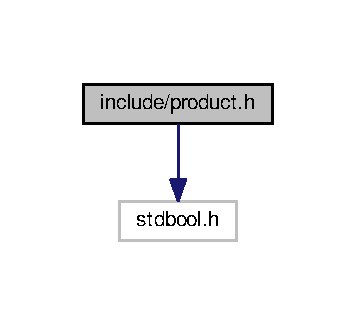
\includegraphics[width=171pt]{product_8h__incl}
\end{center}
\end{figure}
Este grafo mostra quais são os ficheiros que incluem directamente ou indirectamente este ficheiro\+:
\nopagebreak
\begin{figure}[H]
\begin{center}
\leavevmode
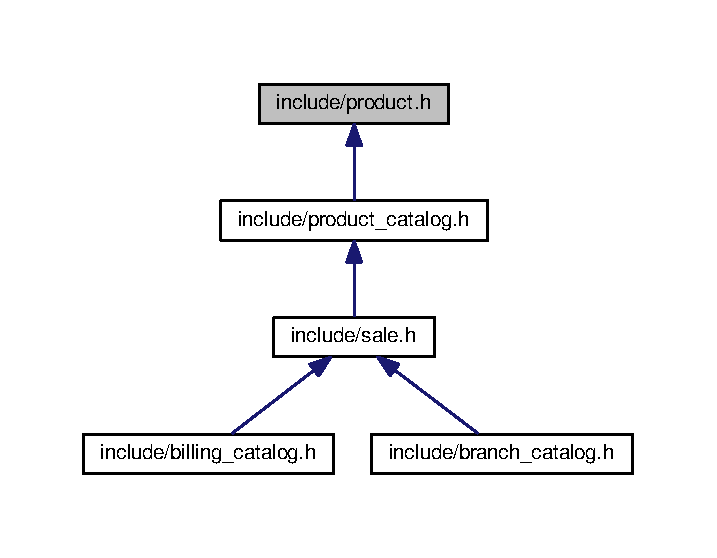
\includegraphics[width=344pt]{product_8h__dep__incl}
\end{center}
\end{figure}
\subsection*{Definições de tipos}
\begin{DoxyCompactItemize}
\item 
\mbox{\Hypertarget{product_8h_a60148a4519d9dd89ced968ddd3d00889}\label{product_8h_a60148a4519d9dd89ced968ddd3d00889}} 
typedef struct \hyperlink{structproduct}{product} $\ast$ {\bfseries Product}
\end{DoxyCompactItemize}
\subsection*{Funções}
\begin{DoxyCompactItemize}
\item 
bool \hyperlink{product_8h_afb94ce2608ae38ca44324a11f93734f4}{verify\+Product} (char $\ast$)
\begin{DoxyCompactList}\small\item\em Devolve um bool consoante o código de produto ser válido ou não. \end{DoxyCompactList}\item 
\hyperlink{structproduct}{Product} \hyperlink{product_8h_adf0011bb7a7d0fd9aac70887fb4193d2}{new\+Product} (char $\ast$)
\begin{DoxyCompactList}\small\item\em Devolve um estrutura Product inicializada com um código de produto. \end{DoxyCompactList}\item 
char $\ast$ \hyperlink{product_8h_a8493a07b192b6c1711a731e9ecefe341}{get\+Product\+Code} (\hyperlink{structproduct}{Product})
\begin{DoxyCompactList}\small\item\em Devolve o código de produto presente na estrutura product. \end{DoxyCompactList}\item 
int \hyperlink{product_8h_a5466f54272944cdfff0c61259d054e8f}{equals\+Product} (\hyperlink{structproduct}{Product}, \hyperlink{structproduct}{Product})
\begin{DoxyCompactList}\small\item\em Verifica a igualdade entre duas estruturas Product dadas. \end{DoxyCompactList}\item 
void \hyperlink{product_8h_abd335e2d660bb3232576d6e14e81a8a3}{destroy\+Product} (\hyperlink{structproduct}{Product})
\begin{DoxyCompactList}\small\item\em Libertar a memória na estrutura Product dada. \end{DoxyCompactList}\end{DoxyCompactItemize}


\subsection{Descrição detalhada}
Módulo de tratamentos de produto. 



\subsection{Documentação das funções}
\mbox{\Hypertarget{product_8h_abd335e2d660bb3232576d6e14e81a8a3}\label{product_8h_abd335e2d660bb3232576d6e14e81a8a3}} 
\index{product.\+h@{product.\+h}!destroy\+Product@{destroy\+Product}}
\index{destroy\+Product@{destroy\+Product}!product.\+h@{product.\+h}}
\subsubsection{\texorpdfstring{destroy\+Product()}{destroyProduct()}}
{\footnotesize\ttfamily void destroy\+Product (\begin{DoxyParamCaption}\item[{\hyperlink{structproduct}{Product}}]{ }\end{DoxyParamCaption})}



Libertar a memória na estrutura Product dada. 


\begin{DoxyParams}{Parâmetros}
{\em product} & Estrutura Product \\
\hline
\end{DoxyParams}
\mbox{\Hypertarget{product_8h_a5466f54272944cdfff0c61259d054e8f}\label{product_8h_a5466f54272944cdfff0c61259d054e8f}} 
\index{product.\+h@{product.\+h}!equals\+Product@{equals\+Product}}
\index{equals\+Product@{equals\+Product}!product.\+h@{product.\+h}}
\subsubsection{\texorpdfstring{equals\+Product()}{equalsProduct()}}
{\footnotesize\ttfamily int equals\+Product (\begin{DoxyParamCaption}\item[{\hyperlink{structproduct}{Product}}]{,  }\item[{\hyperlink{structproduct}{Product}}]{ }\end{DoxyParamCaption})}



Verifica a igualdade entre duas estruturas Product dadas. 


\begin{DoxyParams}{Parâmetros}
{\em a} & Estrutura Product \\
\hline
{\em b} & Estrutura Product \\
\hline
\end{DoxyParams}
\begin{DoxyReturn}{Retorna}
int Número 0 ou 1 
\end{DoxyReturn}
\mbox{\Hypertarget{product_8h_a8493a07b192b6c1711a731e9ecefe341}\label{product_8h_a8493a07b192b6c1711a731e9ecefe341}} 
\index{product.\+h@{product.\+h}!get\+Product\+Code@{get\+Product\+Code}}
\index{get\+Product\+Code@{get\+Product\+Code}!product.\+h@{product.\+h}}
\subsubsection{\texorpdfstring{get\+Product\+Code()}{getProductCode()}}
{\footnotesize\ttfamily char$\ast$ get\+Product\+Code (\begin{DoxyParamCaption}\item[{\hyperlink{structproduct}{Product}}]{ }\end{DoxyParamCaption})}



Devolve o código de produto presente na estrutura product. 


\begin{DoxyParams}{Parâmetros}
{\em Estrutura} & Product \\
\hline
\end{DoxyParams}
\begin{DoxyReturn}{Retorna}
char$\ast$ Código de produto 
\end{DoxyReturn}
\mbox{\Hypertarget{product_8h_adf0011bb7a7d0fd9aac70887fb4193d2}\label{product_8h_adf0011bb7a7d0fd9aac70887fb4193d2}} 
\index{product.\+h@{product.\+h}!new\+Product@{new\+Product}}
\index{new\+Product@{new\+Product}!product.\+h@{product.\+h}}
\subsubsection{\texorpdfstring{new\+Product()}{newProduct()}}
{\footnotesize\ttfamily \hyperlink{structproduct}{Product} new\+Product (\begin{DoxyParamCaption}\item[{char $\ast$}]{ }\end{DoxyParamCaption})}



Devolve um estrutura Product inicializada com um código de produto. 


\begin{DoxyParams}{Parâmetros}
{\em product} & Código de produto \\
\hline
\end{DoxyParams}
\begin{DoxyReturn}{Retorna}
Product Estrutura Product 
\end{DoxyReturn}
\mbox{\Hypertarget{product_8h_afb94ce2608ae38ca44324a11f93734f4}\label{product_8h_afb94ce2608ae38ca44324a11f93734f4}} 
\index{product.\+h@{product.\+h}!verify\+Product@{verify\+Product}}
\index{verify\+Product@{verify\+Product}!product.\+h@{product.\+h}}
\subsubsection{\texorpdfstring{verify\+Product()}{verifyProduct()}}
{\footnotesize\ttfamily bool verify\+Product (\begin{DoxyParamCaption}\item[{char $\ast$}]{ }\end{DoxyParamCaption})}



Devolve um bool consoante o código de produto ser válido ou não. 


\begin{DoxyParams}{Parâmetros}
{\em product} & Código de produto \\
\hline
\end{DoxyParams}
\begin{DoxyReturn}{Retorna}
bool Resultado da verificação 
\end{DoxyReturn}

\hypertarget{product__catalog_8h}{}\section{Referência ao ficheiro include/product\+\_\+catalog.h}
\label{product__catalog_8h}\index{include/product\+\_\+catalog.\+h@{include/product\+\_\+catalog.\+h}}


Módulo de tratamentos do catálogo de produtos.  


{\ttfamily \#include \char`\"{}product.\+h\char`\"{}}\newline
{\ttfamily \#include $<$glib.\+h$>$}\newline
Diagrama de dependências de inclusão para product\+\_\+catalog.\+h\+:
\nopagebreak
\begin{figure}[H]
\begin{center}
\leavevmode
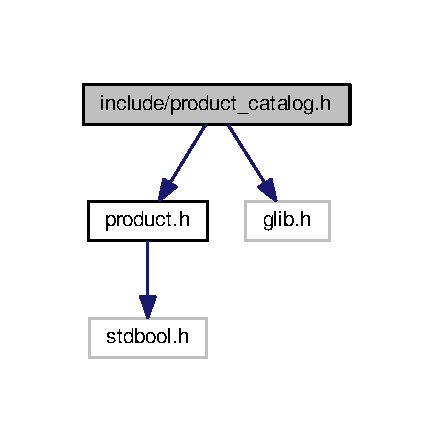
\includegraphics[width=208pt]{product__catalog_8h__incl}
\end{center}
\end{figure}
Este grafo mostra quais são os ficheiros que incluem directamente ou indirectamente este ficheiro\+:
\nopagebreak
\begin{figure}[H]
\begin{center}
\leavevmode
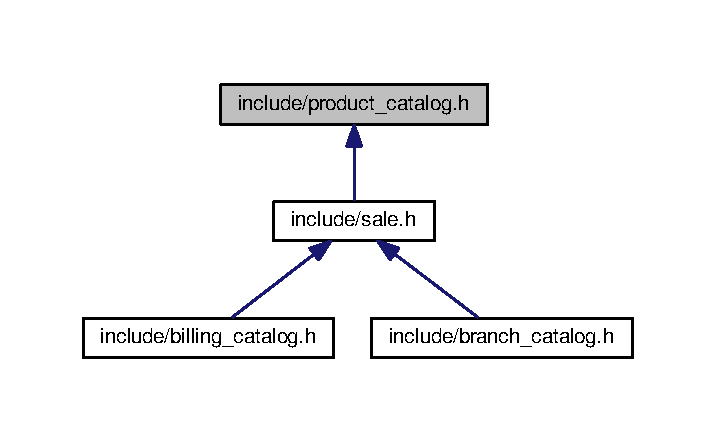
\includegraphics[width=344pt]{product__catalog_8h__dep__incl}
\end{center}
\end{figure}
\subsection*{Definições de tipos}
\begin{DoxyCompactItemize}
\item 
\mbox{\Hypertarget{product__catalog_8h_acc8e68b899b3425203f431ccc419238f}\label{product__catalog_8h_acc8e68b899b3425203f431ccc419238f}} 
typedef struct \hyperlink{structproducts}{products} $\ast$ {\bfseries Products}
\end{DoxyCompactItemize}
\subsection*{Funções}
\begin{DoxyCompactItemize}
\item 
\hyperlink{structproducts}{Products} \hyperlink{product__catalog_8h_a3f6f8e309529e35d9fca74ca39cd0e8f}{init\+Products} ()
\begin{DoxyCompactList}\small\item\em Inicia a estrutura de catálogo de produtos. \end{DoxyCompactList}\item 
char $\ast$$\ast$ \hyperlink{product__catalog_8h_a15eb00397da09786f9779814487ae7cb}{get\+Products\+By\+Letter} (\hyperlink{structproducts}{Products}, char)
\begin{DoxyCompactList}\small\item\em Recolhe todos os produtos que comecem por uma certa letra. \end{DoxyCompactList}\item 
int \hyperlink{product__catalog_8h_ac192082cc23bb95ae1e7abbb8c146d7c}{add\+Product} (\hyperlink{structproducts}{Products}, char $\ast$)
\begin{DoxyCompactList}\small\item\em Adiciona um produto ao catálogo de produto. \end{DoxyCompactList}\item 
int \hyperlink{product__catalog_8h_aeb07b072a6891d1f0a12418a9e0fb632}{get\+Size\+Products} (\hyperlink{structproducts}{Products})
\begin{DoxyCompactList}\small\item\em Calcula o número de produtos que existe no catálogo. \end{DoxyCompactList}\item 
int \hyperlink{product__catalog_8h_a7d67f2f61cb69fd0bf2f6cb9f9433a9a}{exist\+Product} (\hyperlink{structproducts}{Products}, \hyperlink{structproduct}{Product})
\begin{DoxyCompactList}\small\item\em Verifica se existe um produto no catálogo. \end{DoxyCompactList}\item 
void \hyperlink{product__catalog_8h_a4ec8fb7694a4c76fd081c114b824b19c}{destroy\+Products} (\hyperlink{structproducts}{Products})
\begin{DoxyCompactList}\small\item\em Destroi o catálogo de produtos. \end{DoxyCompactList}\item 
char $\ast$$\ast$ \hyperlink{product__catalog_8h_aa5affa0f66b47af6bddead73f8b5b195}{get\+Products\+Not\+Array} (\hyperlink{structproducts}{Products}, G\+Hash\+Table $\ast$)
\begin{DoxyCompactList}\small\item\em Devolve os códigos de produtos que não foram comprados. \end{DoxyCompactList}\item 
int \hyperlink{product__catalog_8h_aa22aba315462d15b96326a981c2d59fc}{get\+Number\+Products\+Not\+Used} (\hyperlink{structproducts}{Products}, G\+Hash\+Table $\ast$)
\begin{DoxyCompactList}\small\item\em Devolve número de código de produtos não utilizados. \end{DoxyCompactList}\item 
int \hyperlink{product__catalog_8h_ad083ec91c88f1db1a9d0a453f9a2adbd}{exist\+Product\+Code} (\hyperlink{structproducts}{Products}, char $\ast$)
\begin{DoxyCompactList}\small\item\em Verifica se existe um código de produto no catálogo. \end{DoxyCompactList}\end{DoxyCompactItemize}


\subsection{Descrição detalhada}
Módulo de tratamentos do catálogo de produtos. 



\subsection{Documentação das funções}
\mbox{\Hypertarget{product__catalog_8h_ac192082cc23bb95ae1e7abbb8c146d7c}\label{product__catalog_8h_ac192082cc23bb95ae1e7abbb8c146d7c}} 
\index{product\+\_\+catalog.\+h@{product\+\_\+catalog.\+h}!add\+Product@{add\+Product}}
\index{add\+Product@{add\+Product}!product\+\_\+catalog.\+h@{product\+\_\+catalog.\+h}}
\subsubsection{\texorpdfstring{add\+Product()}{addProduct()}}
{\footnotesize\ttfamily int add\+Product (\begin{DoxyParamCaption}\item[{\hyperlink{structproducts}{Products}}]{,  }\item[{char $\ast$}]{ }\end{DoxyParamCaption})}



Adiciona um produto ao catálogo de produto. 


\begin{DoxyParams}{Parâmetros}
{\em products} & Catálogo de produtos ao qual vai ser adicionado o novo produto \\
\hline
{\em product} & Cliente a ser adicionado ao catálogo de produtos \\
\hline
\end{DoxyParams}
\begin{DoxyReturn}{Retorna}
int Verificação da inserção 
\end{DoxyReturn}
\mbox{\Hypertarget{product__catalog_8h_a4ec8fb7694a4c76fd081c114b824b19c}\label{product__catalog_8h_a4ec8fb7694a4c76fd081c114b824b19c}} 
\index{product\+\_\+catalog.\+h@{product\+\_\+catalog.\+h}!destroy\+Products@{destroy\+Products}}
\index{destroy\+Products@{destroy\+Products}!product\+\_\+catalog.\+h@{product\+\_\+catalog.\+h}}
\subsubsection{\texorpdfstring{destroy\+Products()}{destroyProducts()}}
{\footnotesize\ttfamily void destroy\+Products (\begin{DoxyParamCaption}\item[{\hyperlink{structproducts}{Products}}]{ }\end{DoxyParamCaption})}



Destroi o catálogo de produtos. 


\begin{DoxyParams}{Parâmetros}
{\em products} & Catálogo de produtos \\
\hline
\end{DoxyParams}
\mbox{\Hypertarget{product__catalog_8h_a7d67f2f61cb69fd0bf2f6cb9f9433a9a}\label{product__catalog_8h_a7d67f2f61cb69fd0bf2f6cb9f9433a9a}} 
\index{product\+\_\+catalog.\+h@{product\+\_\+catalog.\+h}!exist\+Product@{exist\+Product}}
\index{exist\+Product@{exist\+Product}!product\+\_\+catalog.\+h@{product\+\_\+catalog.\+h}}
\subsubsection{\texorpdfstring{exist\+Product()}{existProduct()}}
{\footnotesize\ttfamily int exist\+Product (\begin{DoxyParamCaption}\item[{\hyperlink{structproducts}{Products}}]{,  }\item[{\hyperlink{structproduct}{Product}}]{ }\end{DoxyParamCaption})}



Verifica se existe um produto no catálogo. 


\begin{DoxyParams}{Parâmetros}
{\em products} & Catálogo de produtos \\
\hline
{\em product} & Cliente a ser consultado \\
\hline
\end{DoxyParams}
\begin{DoxyReturn}{Retorna}
int Verificação da procura 
\end{DoxyReturn}
\mbox{\Hypertarget{product__catalog_8h_ad083ec91c88f1db1a9d0a453f9a2adbd}\label{product__catalog_8h_ad083ec91c88f1db1a9d0a453f9a2adbd}} 
\index{product\+\_\+catalog.\+h@{product\+\_\+catalog.\+h}!exist\+Product\+Code@{exist\+Product\+Code}}
\index{exist\+Product\+Code@{exist\+Product\+Code}!product\+\_\+catalog.\+h@{product\+\_\+catalog.\+h}}
\subsubsection{\texorpdfstring{exist\+Product\+Code()}{existProductCode()}}
{\footnotesize\ttfamily int exist\+Product\+Code (\begin{DoxyParamCaption}\item[{\hyperlink{structproducts}{Products}}]{,  }\item[{char $\ast$}]{ }\end{DoxyParamCaption})}



Verifica se existe um código de produto no catálogo. 


\begin{DoxyParams}{Parâmetros}
{\em products} & Catálogo de produtos \\
\hline
{\em product\+\_\+code} & Código de produto \\
\hline
\end{DoxyParams}
\begin{DoxyReturn}{Retorna}
int Verificação da procura 
\end{DoxyReturn}
\mbox{\Hypertarget{product__catalog_8h_aa22aba315462d15b96326a981c2d59fc}\label{product__catalog_8h_aa22aba315462d15b96326a981c2d59fc}} 
\index{product\+\_\+catalog.\+h@{product\+\_\+catalog.\+h}!get\+Number\+Products\+Not\+Used@{get\+Number\+Products\+Not\+Used}}
\index{get\+Number\+Products\+Not\+Used@{get\+Number\+Products\+Not\+Used}!product\+\_\+catalog.\+h@{product\+\_\+catalog.\+h}}
\subsubsection{\texorpdfstring{get\+Number\+Products\+Not\+Used()}{getNumberProductsNotUsed()}}
{\footnotesize\ttfamily int get\+Number\+Products\+Not\+Used (\begin{DoxyParamCaption}\item[{\hyperlink{structproducts}{Products}}]{,  }\item[{G\+Hash\+Table $\ast$}]{ }\end{DoxyParamCaption})}



Devolve número de código de produtos não utilizados. 


\begin{DoxyParams}{Parâmetros}
{\em product\+\_\+catalog} & Catálogo de produtos \\
\hline
{\em products\+\_\+bought} & Hashtable com códigos de produto \\
\hline
\end{DoxyParams}
\begin{DoxyReturn}{Retorna}
int Número de código de produtos não utilizados 
\end{DoxyReturn}
\mbox{\Hypertarget{product__catalog_8h_a15eb00397da09786f9779814487ae7cb}\label{product__catalog_8h_a15eb00397da09786f9779814487ae7cb}} 
\index{product\+\_\+catalog.\+h@{product\+\_\+catalog.\+h}!get\+Products\+By\+Letter@{get\+Products\+By\+Letter}}
\index{get\+Products\+By\+Letter@{get\+Products\+By\+Letter}!product\+\_\+catalog.\+h@{product\+\_\+catalog.\+h}}
\subsubsection{\texorpdfstring{get\+Products\+By\+Letter()}{getProductsByLetter()}}
{\footnotesize\ttfamily char$\ast$$\ast$ get\+Products\+By\+Letter (\begin{DoxyParamCaption}\item[{\hyperlink{structproducts}{Products}}]{,  }\item[{char}]{ }\end{DoxyParamCaption})}



Recolhe todos os produtos que comecem por uma certa letra. 


\begin{DoxyParams}{Parâmetros}
{\em products\+\_\+catalog} & Catálogo de produtos \\
\hline
{\em letter} & Letra pelo qual os produtos começam \\
\hline
\end{DoxyParams}
\begin{DoxyReturn}{Retorna}
char$\ast$$\ast$ Array com todos os códigos de produtos começados pela letra dada 
\end{DoxyReturn}
\mbox{\Hypertarget{product__catalog_8h_aa5affa0f66b47af6bddead73f8b5b195}\label{product__catalog_8h_aa5affa0f66b47af6bddead73f8b5b195}} 
\index{product\+\_\+catalog.\+h@{product\+\_\+catalog.\+h}!get\+Products\+Not\+Array@{get\+Products\+Not\+Array}}
\index{get\+Products\+Not\+Array@{get\+Products\+Not\+Array}!product\+\_\+catalog.\+h@{product\+\_\+catalog.\+h}}
\subsubsection{\texorpdfstring{get\+Products\+Not\+Array()}{getProductsNotArray()}}
{\footnotesize\ttfamily char$\ast$$\ast$ get\+Products\+Not\+Array (\begin{DoxyParamCaption}\item[{\hyperlink{structproducts}{Products}}]{,  }\item[{G\+Hash\+Table $\ast$}]{ }\end{DoxyParamCaption})}



Devolve os códigos de produtos que não foram comprados. 


\begin{DoxyParams}{Parâmetros}
{\em product\+\_\+catalog} & Catálogo de produtos \\
\hline
{\em products\+\_\+bought} & Hashtable com códigos de produto \\
\hline
\end{DoxyParams}
\begin{DoxyReturn}{Retorna}
char$\ast$$\ast$ Array com códigos de produtos 
\end{DoxyReturn}
\mbox{\Hypertarget{product__catalog_8h_aeb07b072a6891d1f0a12418a9e0fb632}\label{product__catalog_8h_aeb07b072a6891d1f0a12418a9e0fb632}} 
\index{product\+\_\+catalog.\+h@{product\+\_\+catalog.\+h}!get\+Size\+Products@{get\+Size\+Products}}
\index{get\+Size\+Products@{get\+Size\+Products}!product\+\_\+catalog.\+h@{product\+\_\+catalog.\+h}}
\subsubsection{\texorpdfstring{get\+Size\+Products()}{getSizeProducts()}}
{\footnotesize\ttfamily int get\+Size\+Products (\begin{DoxyParamCaption}\item[{\hyperlink{structproducts}{Products}}]{ }\end{DoxyParamCaption})}



Calcula o número de produtos que existe no catálogo. 


\begin{DoxyParams}{Parâmetros}
{\em products} & Catálogo de produtos \\
\hline
\end{DoxyParams}
\begin{DoxyReturn}{Retorna}
int Número de produtos existentes no catálogo 
\end{DoxyReturn}
\mbox{\Hypertarget{product__catalog_8h_a3f6f8e309529e35d9fca74ca39cd0e8f}\label{product__catalog_8h_a3f6f8e309529e35d9fca74ca39cd0e8f}} 
\index{product\+\_\+catalog.\+h@{product\+\_\+catalog.\+h}!init\+Products@{init\+Products}}
\index{init\+Products@{init\+Products}!product\+\_\+catalog.\+h@{product\+\_\+catalog.\+h}}
\subsubsection{\texorpdfstring{init\+Products()}{initProducts()}}
{\footnotesize\ttfamily \hyperlink{structproducts}{Products} init\+Products (\begin{DoxyParamCaption}{ }\end{DoxyParamCaption})}



Inicia a estrutura de catálogo de produtos. 

\begin{DoxyReturn}{Retorna}
Products estrutura inicializada 
\end{DoxyReturn}

\hypertarget{sale_8h}{}\section{Referência ao ficheiro include/sale.h}
\label{sale_8h}\index{include/sale.\+h@{include/sale.\+h}}


Módulo de tratamentos de vendas.  


{\ttfamily \#include \char`\"{}product\+\_\+catalog.\+h\char`\"{}}\newline
{\ttfamily \#include \char`\"{}client\+\_\+catalog.\+h\char`\"{}}\newline
Diagrama de dependências de inclusão para sale.\+h\+:
\nopagebreak
\begin{figure}[H]
\begin{center}
\leavevmode
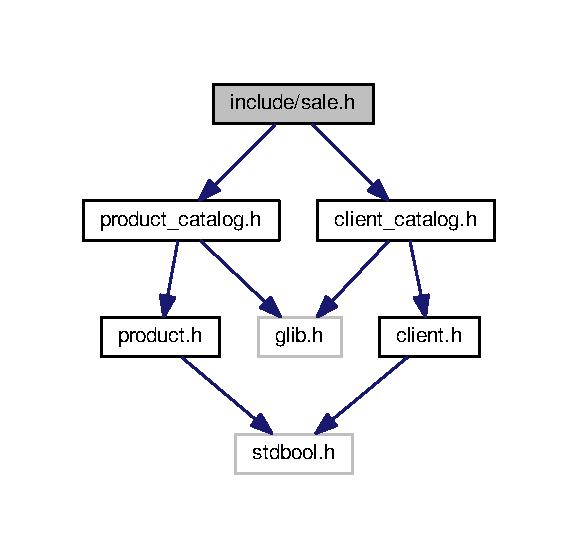
\includegraphics[width=278pt]{sale_8h__incl}
\end{center}
\end{figure}
Este grafo mostra quais são os ficheiros que incluem directamente ou indirectamente este ficheiro\+:
\nopagebreak
\begin{figure}[H]
\begin{center}
\leavevmode
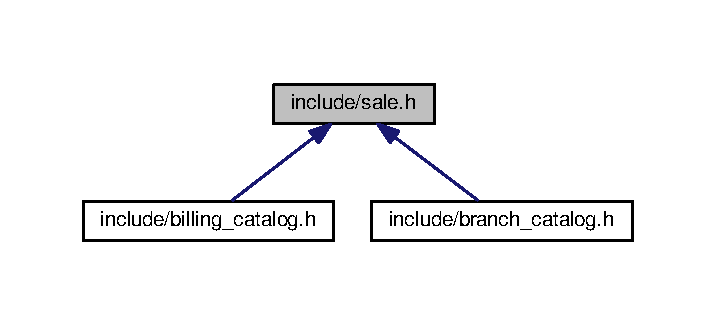
\includegraphics[width=344pt]{sale_8h__dep__incl}
\end{center}
\end{figure}
\subsection*{Definições de tipos}
\begin{DoxyCompactItemize}
\item 
\mbox{\Hypertarget{sale_8h_a5e3050d728070caf3b846252d4da1806}\label{sale_8h_a5e3050d728070caf3b846252d4da1806}} 
typedef struct \hyperlink{structsale}{sale} $\ast$ {\bfseries Sale}
\end{DoxyCompactItemize}
\subsection*{Funções}
\begin{DoxyCompactItemize}
\item 
\hyperlink{structsale}{Sale} \hyperlink{sale_8h_a05f5d59b645d37902e0ba7e419e42eae}{is\+Valid\+Sale} (char $\ast$, \hyperlink{structclients}{Clients}, \hyperlink{structproducts}{Products})
\begin{DoxyCompactList}\small\item\em Devolve uma Sale ou N\+U\+LL consoante a validade da venda. \end{DoxyCompactList}\item 
char $\ast$ \hyperlink{sale_8h_a194c79d8ccb4a6a49ced0fe5ae123f08}{get\+Product} (\hyperlink{structsale}{Sale})
\begin{DoxyCompactList}\small\item\em Devolve o código de produto que foi vendido. \end{DoxyCompactList}\item 
char $\ast$ \hyperlink{sale_8h_a4affad72516432816029136307b4541d}{get\+Client} (\hyperlink{structsale}{Sale})
\begin{DoxyCompactList}\small\item\em Devolve o código de cliente que efetuou a compra. \end{DoxyCompactList}\item 
double \hyperlink{sale_8h_a889c5c0a188d0734575e7214e9b7d7f7}{get\+Price} (\hyperlink{structsale}{Sale})
\begin{DoxyCompactList}\small\item\em Devolve o valor atribuido ao produto na compra. \end{DoxyCompactList}\item 
int \hyperlink{sale_8h_a7ed30b560b4a72819ca298b7ed5d61c0}{get\+Units} (\hyperlink{structsale}{Sale})
\begin{DoxyCompactList}\small\item\em Devolve o número de unidades compradas/vendidas. \end{DoxyCompactList}\item 
char \hyperlink{sale_8h_acb010f4dea79f13390a23ec41efaa0e5}{get\+Promotion} (\hyperlink{structsale}{Sale})
\begin{DoxyCompactList}\small\item\em Devolve o tipo de promoção da compra. \end{DoxyCompactList}\item 
int \hyperlink{sale_8h_ae410306ce25488634136ffecd7a3d46f}{get\+Month} (\hyperlink{structsale}{Sale})
\begin{DoxyCompactList}\small\item\em Devolve o número do mês da compra. \end{DoxyCompactList}\item 
int \hyperlink{sale_8h_ac2f0d82f69847ddeae83fe587c3f28ec}{get\+Branch} (\hyperlink{structsale}{Sale})
\begin{DoxyCompactList}\small\item\em Devolve o número da filial. \end{DoxyCompactList}\item 
void \hyperlink{sale_8h_a9283c6c8006e0781e28c71e57974f7a4}{destroy\+Sale} (\hyperlink{structsale}{Sale})
\begin{DoxyCompactList}\small\item\em Libertar memória na estrutura Sale. \end{DoxyCompactList}\end{DoxyCompactItemize}


\subsection{Descrição detalhada}
Módulo de tratamentos de vendas. 



\subsection{Documentação das funções}
\mbox{\Hypertarget{sale_8h_a9283c6c8006e0781e28c71e57974f7a4}\label{sale_8h_a9283c6c8006e0781e28c71e57974f7a4}} 
\index{sale.\+h@{sale.\+h}!destroy\+Sale@{destroy\+Sale}}
\index{destroy\+Sale@{destroy\+Sale}!sale.\+h@{sale.\+h}}
\subsubsection{\texorpdfstring{destroy\+Sale()}{destroySale()}}
{\footnotesize\ttfamily void destroy\+Sale (\begin{DoxyParamCaption}\item[{\hyperlink{structsale}{Sale}}]{ }\end{DoxyParamCaption})}



Libertar memória na estrutura Sale. 


\begin{DoxyParams}{Parâmetros}
{\em sale} & Estrutura Sale \\
\hline
\end{DoxyParams}
\mbox{\Hypertarget{sale_8h_ac2f0d82f69847ddeae83fe587c3f28ec}\label{sale_8h_ac2f0d82f69847ddeae83fe587c3f28ec}} 
\index{sale.\+h@{sale.\+h}!get\+Branch@{get\+Branch}}
\index{get\+Branch@{get\+Branch}!sale.\+h@{sale.\+h}}
\subsubsection{\texorpdfstring{get\+Branch()}{getBranch()}}
{\footnotesize\ttfamily int get\+Branch (\begin{DoxyParamCaption}\item[{\hyperlink{structsale}{Sale}}]{ }\end{DoxyParamCaption})}



Devolve o número da filial. 


\begin{DoxyParams}{Parâmetros}
{\em sale} & Estrutura Sale \\
\hline
\end{DoxyParams}
\begin{DoxyReturn}{Retorna}
int Número da filial 
\end{DoxyReturn}
\mbox{\Hypertarget{sale_8h_a4affad72516432816029136307b4541d}\label{sale_8h_a4affad72516432816029136307b4541d}} 
\index{sale.\+h@{sale.\+h}!get\+Client@{get\+Client}}
\index{get\+Client@{get\+Client}!sale.\+h@{sale.\+h}}
\subsubsection{\texorpdfstring{get\+Client()}{getClient()}}
{\footnotesize\ttfamily char$\ast$ get\+Client (\begin{DoxyParamCaption}\item[{\hyperlink{structsale}{Sale}}]{ }\end{DoxyParamCaption})}



Devolve o código de cliente que efetuou a compra. 


\begin{DoxyParams}{Parâmetros}
{\em sale} & Estrutura Sale \\
\hline
\end{DoxyParams}
\begin{DoxyReturn}{Retorna}
char$\ast$ Código de cliente 
\end{DoxyReturn}
\mbox{\Hypertarget{sale_8h_ae410306ce25488634136ffecd7a3d46f}\label{sale_8h_ae410306ce25488634136ffecd7a3d46f}} 
\index{sale.\+h@{sale.\+h}!get\+Month@{get\+Month}}
\index{get\+Month@{get\+Month}!sale.\+h@{sale.\+h}}
\subsubsection{\texorpdfstring{get\+Month()}{getMonth()}}
{\footnotesize\ttfamily int get\+Month (\begin{DoxyParamCaption}\item[{\hyperlink{structsale}{Sale}}]{ }\end{DoxyParamCaption})}



Devolve o número do mês da compra. 


\begin{DoxyParams}{Parâmetros}
{\em sale} & Estrutura Sale \\
\hline
\end{DoxyParams}
\begin{DoxyReturn}{Retorna}
int Número do mês da compra 
\end{DoxyReturn}
\mbox{\Hypertarget{sale_8h_a889c5c0a188d0734575e7214e9b7d7f7}\label{sale_8h_a889c5c0a188d0734575e7214e9b7d7f7}} 
\index{sale.\+h@{sale.\+h}!get\+Price@{get\+Price}}
\index{get\+Price@{get\+Price}!sale.\+h@{sale.\+h}}
\subsubsection{\texorpdfstring{get\+Price()}{getPrice()}}
{\footnotesize\ttfamily double get\+Price (\begin{DoxyParamCaption}\item[{\hyperlink{structsale}{Sale}}]{ }\end{DoxyParamCaption})}



Devolve o valor atribuido ao produto na compra. 


\begin{DoxyParams}{Parâmetros}
{\em sale} & Estrutura Sale \\
\hline
\end{DoxyParams}
\begin{DoxyReturn}{Retorna}
double Valor atribuido ao produto na compra 
\end{DoxyReturn}
\mbox{\Hypertarget{sale_8h_a194c79d8ccb4a6a49ced0fe5ae123f08}\label{sale_8h_a194c79d8ccb4a6a49ced0fe5ae123f08}} 
\index{sale.\+h@{sale.\+h}!get\+Product@{get\+Product}}
\index{get\+Product@{get\+Product}!sale.\+h@{sale.\+h}}
\subsubsection{\texorpdfstring{get\+Product()}{getProduct()}}
{\footnotesize\ttfamily char$\ast$ get\+Product (\begin{DoxyParamCaption}\item[{\hyperlink{structsale}{Sale}}]{ }\end{DoxyParamCaption})}



Devolve o código de produto que foi vendido. 


\begin{DoxyParams}{Parâmetros}
{\em sale} & Estrutura Sale \\
\hline
\end{DoxyParams}
\begin{DoxyReturn}{Retorna}
char$\ast$ Código de produto 
\end{DoxyReturn}
\mbox{\Hypertarget{sale_8h_acb010f4dea79f13390a23ec41efaa0e5}\label{sale_8h_acb010f4dea79f13390a23ec41efaa0e5}} 
\index{sale.\+h@{sale.\+h}!get\+Promotion@{get\+Promotion}}
\index{get\+Promotion@{get\+Promotion}!sale.\+h@{sale.\+h}}
\subsubsection{\texorpdfstring{get\+Promotion()}{getPromotion()}}
{\footnotesize\ttfamily char get\+Promotion (\begin{DoxyParamCaption}\item[{\hyperlink{structsale}{Sale}}]{ }\end{DoxyParamCaption})}



Devolve o tipo de promoção da compra. 


\begin{DoxyParams}{Parâmetros}
{\em sale} & Estrutura Sale \\
\hline
\end{DoxyParams}
\begin{DoxyReturn}{Retorna}
char Tipo de promoção da compra N ou P 
\end{DoxyReturn}
\mbox{\Hypertarget{sale_8h_a7ed30b560b4a72819ca298b7ed5d61c0}\label{sale_8h_a7ed30b560b4a72819ca298b7ed5d61c0}} 
\index{sale.\+h@{sale.\+h}!get\+Units@{get\+Units}}
\index{get\+Units@{get\+Units}!sale.\+h@{sale.\+h}}
\subsubsection{\texorpdfstring{get\+Units()}{getUnits()}}
{\footnotesize\ttfamily int get\+Units (\begin{DoxyParamCaption}\item[{\hyperlink{structsale}{Sale}}]{ }\end{DoxyParamCaption})}



Devolve o número de unidades compradas/vendidas. 


\begin{DoxyParams}{Parâmetros}
{\em sale} & Estrutura Sale \\
\hline
\end{DoxyParams}
\begin{DoxyReturn}{Retorna}
int Número de unidades compradas/vendidas 
\end{DoxyReturn}
\mbox{\Hypertarget{sale_8h_a05f5d59b645d37902e0ba7e419e42eae}\label{sale_8h_a05f5d59b645d37902e0ba7e419e42eae}} 
\index{sale.\+h@{sale.\+h}!is\+Valid\+Sale@{is\+Valid\+Sale}}
\index{is\+Valid\+Sale@{is\+Valid\+Sale}!sale.\+h@{sale.\+h}}
\subsubsection{\texorpdfstring{is\+Valid\+Sale()}{isValidSale()}}
{\footnotesize\ttfamily \hyperlink{structsale}{Sale} is\+Valid\+Sale (\begin{DoxyParamCaption}\item[{char $\ast$}]{,  }\item[{\hyperlink{structclients}{Clients}}]{,  }\item[{\hyperlink{structproducts}{Products}}]{ }\end{DoxyParamCaption})}



Devolve uma Sale ou N\+U\+LL consoante a validade da venda. 


\begin{DoxyParams}{Parâmetros}
{\em sale} & Código de venda \\
\hline
{\em client\+\_\+catalogue} & Estrutura Clients \\
\hline
{\em product\+\_\+catalogue} & Products \\
\hline
\end{DoxyParams}
\begin{DoxyReturn}{Retorna}
Sale Estrutura Sale 
\end{DoxyReturn}

\hypertarget{sgv_8h}{}\section{Referência ao ficheiro include/sgv.h}
\label{sgv_8h}\index{include/sgv.\+h@{include/sgv.\+h}}


Módulo de sistema de gestão de vendas.  


{\ttfamily \#include \char`\"{}info.\+h\char`\"{}}\newline
{\ttfamily \#include $<$glib.\+h$>$}\newline
Diagrama de dependências de inclusão para sgv.\+h\+:
\nopagebreak
\begin{figure}[H]
\begin{center}
\leavevmode
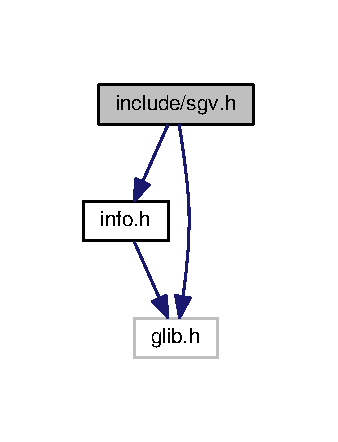
\includegraphics[width=162pt]{sgv_8h__incl}
\end{center}
\end{figure}
\subsection*{Definições de tipos}
\begin{DoxyCompactItemize}
\item 
\mbox{\Hypertarget{sgv_8h_a22f90d0d3126acbfb367c7d5dedbd6b7}\label{sgv_8h_a22f90d0d3126acbfb367c7d5dedbd6b7}} 
typedef struct \hyperlink{structsgv}{sgv} $\ast$ {\bfseries S\+GV}
\item 
\mbox{\Hypertarget{sgv_8h_ad6502ae4eed974fb9646904546f6f02c}\label{sgv_8h_ad6502ae4eed974fb9646904546f6f02c}} 
typedef struct \hyperlink{structstartValues}{start\+Values} $\ast$ {\bfseries Start\+Values}
\end{DoxyCompactItemize}
\subsection*{Funções}
\begin{DoxyCompactItemize}
\item 
\hyperlink{structsgv}{S\+GV} \hyperlink{sgv_8h_a9efc223dce291c384b94e9fd8674d319}{start\+S\+GV} (\hyperlink{structsgv}{S\+GV}, \hyperlink{structstartValues}{Start\+Values})
\begin{DoxyCompactList}\small\item\em Devolve a estrutura S\+GV com o conteúdo dos ficheiros dados. \end{DoxyCompactList}\item 
\hyperlink{structsgv}{S\+GV} \hyperlink{sgv_8h_a14c3840c38c574667ca887b40c5250bb}{init\+S\+GV} ()
\begin{DoxyCompactList}\small\item\em Devolve a estrutura S\+GV inicializada. \end{DoxyCompactList}\item 
\hyperlink{structstartValues}{Start\+Values} \hyperlink{sgv_8h_ab8599dd4fc511628421653597fede4d3}{init\+Start\+Values} ()
\begin{DoxyCompactList}\small\item\em Devolve a estrutura Start\+Values inicializada. \end{DoxyCompactList}\item 
void \hyperlink{sgv_8h_ac13cac74a32f7c3032bd0cc5cde2c049}{set\+Paths\+SV} (\hyperlink{structstartValues}{Start\+Values}, char $\ast$, char $\ast$, char $\ast$)
\begin{DoxyCompactList}\small\item\em Devolve a estrutura S\+GV com o conteúdo dos ficheiros dados. \end{DoxyCompactList}\item 
char $\ast$$\ast$ \hyperlink{sgv_8h_ac0c7868d4a31bbae5ffa9b30dad3f9ce}{get\+Products\+Started\+By\+Letter} (\hyperlink{structsgv}{S\+GV}, char)
\begin{DoxyCompactList}\small\item\em Devolve o número total de vendas e o total facturado com esse produto em tal mês, distinguindo os totais em modo N e os totais em modo P. \end{DoxyCompactList}\item 
double $\ast$ \hyperlink{sgv_8h_a9d13c6476f5db5c398ffed5b21d25333}{get\+Product\+Sales\+And\+Profit} (\hyperlink{structsgv}{S\+GV}, char $\ast$, int, int)
\begin{DoxyCompactList}\small\item\em Devolve todos os códigos de produto que começam com uma certa letra. \end{DoxyCompactList}\item 
char $\ast$$\ast$$\ast$ \hyperlink{sgv_8h_a338dc1702caf4ff8af1f20e9eff96256}{get\+Products\+Never\+Bought} (\hyperlink{structsgv}{S\+GV}, int)
\begin{DoxyCompactList}\small\item\em Devolve a lista ordenada dos códigos dos produtos(e o seu número total)que ninguém comprou, podendo o utilizador decidir igualmente se pretende valores totais ou divididos pelas filiais. \end{DoxyCompactList}\item 
char $\ast$$\ast$ \hyperlink{sgv_8h_a8fc177229f098ba892b1267635d31e13}{get\+Clients\+Of\+All\+Branches} (\hyperlink{structsgv}{S\+GV})
\begin{DoxyCompactList}\small\item\em Devolve a lista ordenada de códigos de clientes que realizaram compras em todas as filiais. \end{DoxyCompactList}\item 
int $\ast$ \hyperlink{sgv_8h_a2057daf05b0769167711e6f85205bba6}{get\+Clients\+And\+Products\+Never\+Bought\+Count} (\hyperlink{structsgv}{S\+GV})
\begin{DoxyCompactList}\small\item\em Devolve o número de clientes registados que não realizaram compras bem como o número de produtos que ninguém comprou. \end{DoxyCompactList}\item 
int $\ast$$\ast$ \hyperlink{sgv_8h_aecbd0f7b01ba462926af9ab06ca57565}{get\+Products\+Bought\+By\+Client} (\hyperlink{structsgv}{S\+GV}, char $\ast$)
\begin{DoxyCompactList}\small\item\em Devolve o número total de produtos comprados por um certos cliente mês a mês organizado por filial. \end{DoxyCompactList}\item 
\hyperlink{structquerie8Aux}{Query8\+Aux} \hyperlink{sgv_8h_a52ce4c6daa90f4c9dfcbd167be408993}{get\+Sales\+And\+Profit} (\hyperlink{structsgv}{S\+GV}, int, int)
\begin{DoxyCompactList}\small\item\em Devolve o total de vendas(nº de registos de venda) registado num intervalo de meses e o total faturado. \end{DoxyCompactList}\item 
\hyperlink{structquerie9Aux}{Query9\+Aux} \hyperlink{sgv_8h_ad98774690dfae0b44935208e6e7b6e3f}{get\+Product\+Buyers} (\hyperlink{structsgv}{S\+GV}, char $\ast$, int)
\begin{DoxyCompactList}\small\item\em Devolve os códigos (e número total) dos clientes que o compraram, distinguindo entre compra N e compra P. \end{DoxyCompactList}\item 
\hyperlink{structinfo}{Info} $\ast$ \hyperlink{sgv_8h_a5232d7ae7a7ef5601cf264ff55e3648a}{get\+Clients\+Favorite\+Products} (\hyperlink{structsgv}{S\+GV}, char $\ast$, int)
\begin{DoxyCompactList}\small\item\em Devolve uma lista por ordem descendente de códigos de produtos que um dado cliente mais comprou num mês, por quantidade e não por faturação. \end{DoxyCompactList}\item 
\hyperlink{structaux}{Aux} $\ast$ \hyperlink{sgv_8h_a352401261457e19136f0ba66240bdd8b}{get\+Top\+Sold\+Products} (\hyperlink{structsgv}{S\+GV}, int)
\begin{DoxyCompactList}\small\item\em Devolve uma lista dos N produtos mais vendidos em todo o ano, indicando o número total de clientes eo número de unidades vendidas, filial a filial. \end{DoxyCompactList}\item 
\hyperlink{structmoney}{Money} $\ast$ \hyperlink{sgv_8h_a336905bf5814c04523d5611cc57b8c8a}{get\+Client\+Top\+Profit\+Products} (\hyperlink{structsgv}{S\+GV}, char $\ast$, int)
\begin{DoxyCompactList}\small\item\em Devolve os códigos dos N produtos em que um dado cliente mais gastou(dinheiro) durante o ano. \end{DoxyCompactList}\item 
char $\ast$ \hyperlink{sgv_8h_ae53b11a41fe660b4890199213a0ca0f3}{get\+Clients\+Path} (\hyperlink{structstartValues}{Start\+Values})
\begin{DoxyCompactList}\small\item\em Devolver o path do ficheiro de clientes. \end{DoxyCompactList}\item 
char $\ast$ \hyperlink{sgv_8h_a02575af4cacc490db462d85617a1b385}{get\+Products\+Path} (\hyperlink{structstartValues}{Start\+Values})
\begin{DoxyCompactList}\small\item\em Devolver o path do ficheiro de produtos. \end{DoxyCompactList}\item 
char $\ast$ \hyperlink{sgv_8h_a4056766d419e42860012a2207f2b7e0a}{get\+Sales\+Path} (\hyperlink{structstartValues}{Start\+Values})
\begin{DoxyCompactList}\small\item\em Devolver o path do ficheiro de vendas. \end{DoxyCompactList}\item 
int \hyperlink{sgv_8h_a100e8d9788b8f6d202398c0f43a93221}{get\+Valid\+Clients} (\hyperlink{structstartValues}{Start\+Values})
\begin{DoxyCompactList}\small\item\em Devolver o número de clientes válidos no ficheiro de clientes. \end{DoxyCompactList}\item 
int \hyperlink{sgv_8h_acee7a37d1a1f48711fda3f11ea51f437}{get\+Valid\+Products} (\hyperlink{structstartValues}{Start\+Values})
\begin{DoxyCompactList}\small\item\em Devolver o número de clientes válidos no ficheiro de produtos. \end{DoxyCompactList}\item 
int \hyperlink{sgv_8h_ad84fb04ca88251beaee348c20754e69a}{get\+Valid\+Sales} (\hyperlink{structstartValues}{Start\+Values})
\begin{DoxyCompactList}\small\item\em Devolver o número de clientes válidos no ficheiro de vendas. \end{DoxyCompactList}\item 
int \hyperlink{sgv_8h_a22de448d77ae7e07453a78393243e286}{get\+Read\+Clients} (\hyperlink{structstartValues}{Start\+Values})
\begin{DoxyCompactList}\small\item\em Devolver o número de clientes lidos no ficheiro de clientes. \end{DoxyCompactList}\item 
int \hyperlink{sgv_8h_a88b6aab95c077c921ba483d33e006706}{get\+Read\+Products} (\hyperlink{structstartValues}{Start\+Values})
\begin{DoxyCompactList}\small\item\em Devolver o número de produtos lidos no ficheiro de produtos. \end{DoxyCompactList}\item 
int \hyperlink{sgv_8h_ad68bbdec54a428df9f32bd82733a8a56}{get\+Read\+Sales} (\hyperlink{structstartValues}{Start\+Values})
\begin{DoxyCompactList}\small\item\em Devolver o número de vendas lidos no ficheiro de vendas. \end{DoxyCompactList}\item 
int \hyperlink{sgv_8h_a83d57b21fdf3420e131d6572414649ff}{list\+Size} (char $\ast$$\ast$)
\begin{DoxyCompactList}\small\item\em Devolver o tamanho de um Array de strings(char$\ast$) \end{DoxyCompactList}\item 
void \hyperlink{sgv_8h_aea864ae993f31c9a0ce9242ff9e6e045}{destroy\+S\+GV} (\hyperlink{structsgv}{S\+GV})
\begin{DoxyCompactList}\small\item\em Libertar memória na estrutura S\+GV. \end{DoxyCompactList}\item 
void \hyperlink{sgv_8h_a1e8bd065f8893f145b91182e4c595f66}{destroy\+Start\+Values} (\hyperlink{structstartValues}{Start\+Values})
\begin{DoxyCompactList}\small\item\em Libertar memória na estrutura Start\+Values. \end{DoxyCompactList}\item 
void \hyperlink{sgv_8h_a4883e13e3eff8496e29a5e4b80ee21c5}{free\+String\+List} (char $\ast$$\ast$)
\begin{DoxyCompactList}\small\item\em Libertar memória alocada no array. \end{DoxyCompactList}\item 
void \hyperlink{sgv_8h_aab218747277284f303800dbb826c2d65}{free\+String\+Matrix} (char $\ast$$\ast$$\ast$)
\begin{DoxyCompactList}\small\item\em Libertar memória alocada na matriz. \end{DoxyCompactList}\item 
void \hyperlink{sgv_8h_a082869997a6c7f8668f8261754640a87}{free\+Int\+Matrix} (int $\ast$$\ast$)
\begin{DoxyCompactList}\small\item\em Libertar memória alocada na matriz. \end{DoxyCompactList}\end{DoxyCompactItemize}


\subsection{Descrição detalhada}
Módulo de sistema de gestão de vendas. 



\subsection{Documentação das funções}
\mbox{\Hypertarget{sgv_8h_aea864ae993f31c9a0ce9242ff9e6e045}\label{sgv_8h_aea864ae993f31c9a0ce9242ff9e6e045}} 
\index{sgv.\+h@{sgv.\+h}!destroy\+S\+GV@{destroy\+S\+GV}}
\index{destroy\+S\+GV@{destroy\+S\+GV}!sgv.\+h@{sgv.\+h}}
\subsubsection{\texorpdfstring{destroy\+S\+G\+V()}{destroySGV()}}
{\footnotesize\ttfamily void destroy\+S\+GV (\begin{DoxyParamCaption}\item[{\hyperlink{structsgv}{S\+GV}}]{ }\end{DoxyParamCaption})}



Libertar memória na estrutura S\+GV. 


\begin{DoxyParams}{Parâmetros}
{\em sgv} & Estrutura S\+GV \\
\hline
\end{DoxyParams}
\mbox{\Hypertarget{sgv_8h_a1e8bd065f8893f145b91182e4c595f66}\label{sgv_8h_a1e8bd065f8893f145b91182e4c595f66}} 
\index{sgv.\+h@{sgv.\+h}!destroy\+Start\+Values@{destroy\+Start\+Values}}
\index{destroy\+Start\+Values@{destroy\+Start\+Values}!sgv.\+h@{sgv.\+h}}
\subsubsection{\texorpdfstring{destroy\+Start\+Values()}{destroyStartValues()}}
{\footnotesize\ttfamily void destroy\+Start\+Values (\begin{DoxyParamCaption}\item[{\hyperlink{structstartValues}{Start\+Values}}]{ }\end{DoxyParamCaption})}



Libertar memória na estrutura Start\+Values. 


\begin{DoxyParams}{Parâmetros}
{\em sv} & Estrutura Start\+Values \\
\hline
\end{DoxyParams}
\mbox{\Hypertarget{sgv_8h_a082869997a6c7f8668f8261754640a87}\label{sgv_8h_a082869997a6c7f8668f8261754640a87}} 
\index{sgv.\+h@{sgv.\+h}!free\+Int\+Matrix@{free\+Int\+Matrix}}
\index{free\+Int\+Matrix@{free\+Int\+Matrix}!sgv.\+h@{sgv.\+h}}
\subsubsection{\texorpdfstring{free\+Int\+Matrix()}{freeIntMatrix()}}
{\footnotesize\ttfamily void free\+Int\+Matrix (\begin{DoxyParamCaption}\item[{int $\ast$$\ast$}]{ }\end{DoxyParamCaption})}



Libertar memória alocada na matriz. 


\begin{DoxyParams}{Parâmetros}
{\em matrix} & Array com arrays de int \\
\hline
\end{DoxyParams}
\mbox{\Hypertarget{sgv_8h_a4883e13e3eff8496e29a5e4b80ee21c5}\label{sgv_8h_a4883e13e3eff8496e29a5e4b80ee21c5}} 
\index{sgv.\+h@{sgv.\+h}!free\+String\+List@{free\+String\+List}}
\index{free\+String\+List@{free\+String\+List}!sgv.\+h@{sgv.\+h}}
\subsubsection{\texorpdfstring{free\+String\+List()}{freeStringList()}}
{\footnotesize\ttfamily void free\+String\+List (\begin{DoxyParamCaption}\item[{char $\ast$$\ast$}]{ }\end{DoxyParamCaption})}



Libertar memória alocada no array. 


\begin{DoxyParams}{Parâmetros}
{\em list} & Array de strings(char$\ast$) \\
\hline
\end{DoxyParams}
\mbox{\Hypertarget{sgv_8h_aab218747277284f303800dbb826c2d65}\label{sgv_8h_aab218747277284f303800dbb826c2d65}} 
\index{sgv.\+h@{sgv.\+h}!free\+String\+Matrix@{free\+String\+Matrix}}
\index{free\+String\+Matrix@{free\+String\+Matrix}!sgv.\+h@{sgv.\+h}}
\subsubsection{\texorpdfstring{free\+String\+Matrix()}{freeStringMatrix()}}
{\footnotesize\ttfamily void free\+String\+Matrix (\begin{DoxyParamCaption}\item[{char $\ast$$\ast$$\ast$}]{ }\end{DoxyParamCaption})}



Libertar memória alocada na matriz. 


\begin{DoxyParams}{Parâmetros}
{\em matrix} & Array com arrays de strings(char$\ast$) \\
\hline
\end{DoxyParams}
\mbox{\Hypertarget{sgv_8h_a2057daf05b0769167711e6f85205bba6}\label{sgv_8h_a2057daf05b0769167711e6f85205bba6}} 
\index{sgv.\+h@{sgv.\+h}!get\+Clients\+And\+Products\+Never\+Bought\+Count@{get\+Clients\+And\+Products\+Never\+Bought\+Count}}
\index{get\+Clients\+And\+Products\+Never\+Bought\+Count@{get\+Clients\+And\+Products\+Never\+Bought\+Count}!sgv.\+h@{sgv.\+h}}
\subsubsection{\texorpdfstring{get\+Clients\+And\+Products\+Never\+Bought\+Count()}{getClientsAndProductsNeverBoughtCount()}}
{\footnotesize\ttfamily int$\ast$ get\+Clients\+And\+Products\+Never\+Bought\+Count (\begin{DoxyParamCaption}\item[{\hyperlink{structsgv}{S\+GV}}]{ }\end{DoxyParamCaption})}



Devolve o número de clientes registados que não realizaram compras bem como o número de produtos que ninguém comprou. 


\begin{DoxyParams}{Parâmetros}
{\em sgv} & Estrutura S\+GV \\
\hline
\end{DoxyParams}
\begin{DoxyReturn}{Retorna}
int$\ast$ Array de ints 
\end{DoxyReturn}
\mbox{\Hypertarget{sgv_8h_a5232d7ae7a7ef5601cf264ff55e3648a}\label{sgv_8h_a5232d7ae7a7ef5601cf264ff55e3648a}} 
\index{sgv.\+h@{sgv.\+h}!get\+Clients\+Favorite\+Products@{get\+Clients\+Favorite\+Products}}
\index{get\+Clients\+Favorite\+Products@{get\+Clients\+Favorite\+Products}!sgv.\+h@{sgv.\+h}}
\subsubsection{\texorpdfstring{get\+Clients\+Favorite\+Products()}{getClientsFavoriteProducts()}}
{\footnotesize\ttfamily \hyperlink{structinfo}{Info}$\ast$ get\+Clients\+Favorite\+Products (\begin{DoxyParamCaption}\item[{\hyperlink{structsgv}{S\+GV}}]{,  }\item[{char $\ast$}]{,  }\item[{int}]{ }\end{DoxyParamCaption})}



Devolve uma lista por ordem descendente de códigos de produtos que um dado cliente mais comprou num mês, por quantidade e não por faturação. 


\begin{DoxyParams}{Parâmetros}
{\em sgv} & Estrutura S\+GV \\
\hline
{\em client\+\_\+code} & Código de cliente \\
\hline
{\em month} & Número da mês \\
\hline
\end{DoxyParams}
\begin{DoxyReturn}{Retorna}
Info$\ast$ Array de estruturas Info 
\end{DoxyReturn}
\mbox{\Hypertarget{sgv_8h_a8fc177229f098ba892b1267635d31e13}\label{sgv_8h_a8fc177229f098ba892b1267635d31e13}} 
\index{sgv.\+h@{sgv.\+h}!get\+Clients\+Of\+All\+Branches@{get\+Clients\+Of\+All\+Branches}}
\index{get\+Clients\+Of\+All\+Branches@{get\+Clients\+Of\+All\+Branches}!sgv.\+h@{sgv.\+h}}
\subsubsection{\texorpdfstring{get\+Clients\+Of\+All\+Branches()}{getClientsOfAllBranches()}}
{\footnotesize\ttfamily char$\ast$$\ast$ get\+Clients\+Of\+All\+Branches (\begin{DoxyParamCaption}\item[{\hyperlink{structsgv}{S\+GV}}]{ }\end{DoxyParamCaption})}



Devolve a lista ordenada de códigos de clientes que realizaram compras em todas as filiais. 


\begin{DoxyParams}{Parâmetros}
{\em sgv} & Estrutura S\+GV \\
\hline
\end{DoxyParams}
\begin{DoxyReturn}{Retorna}
char$\ast$$\ast$ Array com códigos de clientes 
\end{DoxyReturn}
\mbox{\Hypertarget{sgv_8h_ae53b11a41fe660b4890199213a0ca0f3}\label{sgv_8h_ae53b11a41fe660b4890199213a0ca0f3}} 
\index{sgv.\+h@{sgv.\+h}!get\+Clients\+Path@{get\+Clients\+Path}}
\index{get\+Clients\+Path@{get\+Clients\+Path}!sgv.\+h@{sgv.\+h}}
\subsubsection{\texorpdfstring{get\+Clients\+Path()}{getClientsPath()}}
{\footnotesize\ttfamily char$\ast$ get\+Clients\+Path (\begin{DoxyParamCaption}\item[{\hyperlink{structstartValues}{Start\+Values}}]{ }\end{DoxyParamCaption})}



Devolver o path do ficheiro de clientes. 


\begin{DoxyParams}{Parâmetros}
{\em sv} & Estrutura Start\+Values \\
\hline
\end{DoxyParams}
\begin{DoxyReturn}{Retorna}
char$\ast$ Path do ficheiro de clientes 
\end{DoxyReturn}
\mbox{\Hypertarget{sgv_8h_a336905bf5814c04523d5611cc57b8c8a}\label{sgv_8h_a336905bf5814c04523d5611cc57b8c8a}} 
\index{sgv.\+h@{sgv.\+h}!get\+Client\+Top\+Profit\+Products@{get\+Client\+Top\+Profit\+Products}}
\index{get\+Client\+Top\+Profit\+Products@{get\+Client\+Top\+Profit\+Products}!sgv.\+h@{sgv.\+h}}
\subsubsection{\texorpdfstring{get\+Client\+Top\+Profit\+Products()}{getClientTopProfitProducts()}}
{\footnotesize\ttfamily \hyperlink{structmoney}{Money}$\ast$ get\+Client\+Top\+Profit\+Products (\begin{DoxyParamCaption}\item[{\hyperlink{structsgv}{S\+GV}}]{,  }\item[{char $\ast$}]{,  }\item[{int}]{ }\end{DoxyParamCaption})}



Devolve os códigos dos N produtos em que um dado cliente mais gastou(dinheiro) durante o ano. 


\begin{DoxyParams}{Parâmetros}
{\em sgv} & Estrutura S\+GV \\
\hline
{\em client\+\_\+code} & Código de cliente \\
\hline
{\em n} & Número de produtos \\
\hline
\end{DoxyParams}
\begin{DoxyReturn}{Retorna}
Money$\ast$ Array de estruturas Money 
\end{DoxyReturn}
\mbox{\Hypertarget{sgv_8h_ad98774690dfae0b44935208e6e7b6e3f}\label{sgv_8h_ad98774690dfae0b44935208e6e7b6e3f}} 
\index{sgv.\+h@{sgv.\+h}!get\+Product\+Buyers@{get\+Product\+Buyers}}
\index{get\+Product\+Buyers@{get\+Product\+Buyers}!sgv.\+h@{sgv.\+h}}
\subsubsection{\texorpdfstring{get\+Product\+Buyers()}{getProductBuyers()}}
{\footnotesize\ttfamily \hyperlink{structquerie9Aux}{Query9\+Aux} get\+Product\+Buyers (\begin{DoxyParamCaption}\item[{\hyperlink{structsgv}{S\+GV}}]{,  }\item[{char $\ast$}]{,  }\item[{int}]{ }\end{DoxyParamCaption})}



Devolve os códigos (e número total) dos clientes que o compraram, distinguindo entre compra N e compra P. 


\begin{DoxyParams}{Parâmetros}
{\em sgv} & Estrutura S\+GV \\
\hline
{\em product\+\_\+code} & Código de produto \\
\hline
{\em branch} & Número da filial \\
\hline
\end{DoxyParams}
\begin{DoxyReturn}{Retorna}
Query9\+Aux Estrutura Query9\+Aux 
\end{DoxyReturn}
\mbox{\Hypertarget{sgv_8h_a9d13c6476f5db5c398ffed5b21d25333}\label{sgv_8h_a9d13c6476f5db5c398ffed5b21d25333}} 
\index{sgv.\+h@{sgv.\+h}!get\+Product\+Sales\+And\+Profit@{get\+Product\+Sales\+And\+Profit}}
\index{get\+Product\+Sales\+And\+Profit@{get\+Product\+Sales\+And\+Profit}!sgv.\+h@{sgv.\+h}}
\subsubsection{\texorpdfstring{get\+Product\+Sales\+And\+Profit()}{getProductSalesAndProfit()}}
{\footnotesize\ttfamily double$\ast$ get\+Product\+Sales\+And\+Profit (\begin{DoxyParamCaption}\item[{\hyperlink{structsgv}{S\+GV}}]{,  }\item[{char $\ast$}]{,  }\item[{int}]{,  }\item[{int}]{ }\end{DoxyParamCaption})}



Devolve todos os códigos de produto que começam com uma certa letra. 


\begin{DoxyParams}{Parâmetros}
{\em sgv} & Estrutura S\+GV \\
\hline
{\em product\+\_\+code} & Código de produto \\
\hline
{\em month} & Número do mês \\
\hline
{\em branches} & Filial \\
\hline
\end{DoxyParams}
\begin{DoxyReturn}{Retorna}
double$\ast$ Path do ficheiro de vendas 
\end{DoxyReturn}
\mbox{\Hypertarget{sgv_8h_aecbd0f7b01ba462926af9ab06ca57565}\label{sgv_8h_aecbd0f7b01ba462926af9ab06ca57565}} 
\index{sgv.\+h@{sgv.\+h}!get\+Products\+Bought\+By\+Client@{get\+Products\+Bought\+By\+Client}}
\index{get\+Products\+Bought\+By\+Client@{get\+Products\+Bought\+By\+Client}!sgv.\+h@{sgv.\+h}}
\subsubsection{\texorpdfstring{get\+Products\+Bought\+By\+Client()}{getProductsBoughtByClient()}}
{\footnotesize\ttfamily int$\ast$$\ast$ get\+Products\+Bought\+By\+Client (\begin{DoxyParamCaption}\item[{\hyperlink{structsgv}{S\+GV}}]{,  }\item[{char $\ast$}]{ }\end{DoxyParamCaption})}



Devolve o número total de produtos comprados por um certos cliente mês a mês organizado por filial. 


\begin{DoxyParams}{Parâmetros}
{\em sgv} & Estrutura S\+GV \\
\hline
{\em client\+\_\+code} & Código de cliente \\
\hline
\end{DoxyParams}
\begin{DoxyReturn}{Retorna}
int$\ast$$\ast$ Array de ints 
\end{DoxyReturn}
\mbox{\Hypertarget{sgv_8h_a338dc1702caf4ff8af1f20e9eff96256}\label{sgv_8h_a338dc1702caf4ff8af1f20e9eff96256}} 
\index{sgv.\+h@{sgv.\+h}!get\+Products\+Never\+Bought@{get\+Products\+Never\+Bought}}
\index{get\+Products\+Never\+Bought@{get\+Products\+Never\+Bought}!sgv.\+h@{sgv.\+h}}
\subsubsection{\texorpdfstring{get\+Products\+Never\+Bought()}{getProductsNeverBought()}}
{\footnotesize\ttfamily char$\ast$$\ast$$\ast$ get\+Products\+Never\+Bought (\begin{DoxyParamCaption}\item[{\hyperlink{structsgv}{S\+GV}}]{,  }\item[{int}]{ }\end{DoxyParamCaption})}



Devolve a lista ordenada dos códigos dos produtos(e o seu número total)que ninguém comprou, podendo o utilizador decidir igualmente se pretende valores totais ou divididos pelas filiais. 


\begin{DoxyParams}{Parâmetros}
{\em sgv} & Estrutura S\+GV \\
\hline
{\em is\+Global} & Número que representa modo global ou uma filial \\
\hline
\end{DoxyParams}
\begin{DoxyReturn}{Retorna}
char$\ast$$\ast$$\ast$ Array com Arrays de códigos de produtos 
\end{DoxyReturn}
\mbox{\Hypertarget{sgv_8h_a02575af4cacc490db462d85617a1b385}\label{sgv_8h_a02575af4cacc490db462d85617a1b385}} 
\index{sgv.\+h@{sgv.\+h}!get\+Products\+Path@{get\+Products\+Path}}
\index{get\+Products\+Path@{get\+Products\+Path}!sgv.\+h@{sgv.\+h}}
\subsubsection{\texorpdfstring{get\+Products\+Path()}{getProductsPath()}}
{\footnotesize\ttfamily char$\ast$ get\+Products\+Path (\begin{DoxyParamCaption}\item[{\hyperlink{structstartValues}{Start\+Values}}]{ }\end{DoxyParamCaption})}



Devolver o path do ficheiro de produtos. 


\begin{DoxyParams}{Parâmetros}
{\em sv} & Estrutura Start\+Values \\
\hline
\end{DoxyParams}
\begin{DoxyReturn}{Retorna}
char$\ast$ Path do ficheiro de produtos 
\end{DoxyReturn}
\mbox{\Hypertarget{sgv_8h_ac0c7868d4a31bbae5ffa9b30dad3f9ce}\label{sgv_8h_ac0c7868d4a31bbae5ffa9b30dad3f9ce}} 
\index{sgv.\+h@{sgv.\+h}!get\+Products\+Started\+By\+Letter@{get\+Products\+Started\+By\+Letter}}
\index{get\+Products\+Started\+By\+Letter@{get\+Products\+Started\+By\+Letter}!sgv.\+h@{sgv.\+h}}
\subsubsection{\texorpdfstring{get\+Products\+Started\+By\+Letter()}{getProductsStartedByLetter()}}
{\footnotesize\ttfamily char$\ast$$\ast$ get\+Products\+Started\+By\+Letter (\begin{DoxyParamCaption}\item[{\hyperlink{structsgv}{S\+GV}}]{,  }\item[{char}]{ }\end{DoxyParamCaption})}



Devolve o número total de vendas e o total facturado com esse produto em tal mês, distinguindo os totais em modo N e os totais em modo P. 


\begin{DoxyParams}{Parâmetros}
{\em sgv} & Estrutura S\+GV \\
\hline
{\em letter} & Letra entre A a Z \\
\hline
\end{DoxyParams}
\begin{DoxyReturn}{Retorna}
char$\ast$$\ast$ Path do ficheiro de vendas 
\end{DoxyReturn}
\mbox{\Hypertarget{sgv_8h_a22de448d77ae7e07453a78393243e286}\label{sgv_8h_a22de448d77ae7e07453a78393243e286}} 
\index{sgv.\+h@{sgv.\+h}!get\+Read\+Clients@{get\+Read\+Clients}}
\index{get\+Read\+Clients@{get\+Read\+Clients}!sgv.\+h@{sgv.\+h}}
\subsubsection{\texorpdfstring{get\+Read\+Clients()}{getReadClients()}}
{\footnotesize\ttfamily int get\+Read\+Clients (\begin{DoxyParamCaption}\item[{\hyperlink{structstartValues}{Start\+Values}}]{ }\end{DoxyParamCaption})}



Devolver o número de clientes lidos no ficheiro de clientes. 


\begin{DoxyParams}{Parâmetros}
{\em sv} & Estrutura Start\+Values \\
\hline
\end{DoxyParams}
\begin{DoxyReturn}{Retorna}
int Número de clientes lidos 
\end{DoxyReturn}
\mbox{\Hypertarget{sgv_8h_a88b6aab95c077c921ba483d33e006706}\label{sgv_8h_a88b6aab95c077c921ba483d33e006706}} 
\index{sgv.\+h@{sgv.\+h}!get\+Read\+Products@{get\+Read\+Products}}
\index{get\+Read\+Products@{get\+Read\+Products}!sgv.\+h@{sgv.\+h}}
\subsubsection{\texorpdfstring{get\+Read\+Products()}{getReadProducts()}}
{\footnotesize\ttfamily int get\+Read\+Products (\begin{DoxyParamCaption}\item[{\hyperlink{structstartValues}{Start\+Values}}]{ }\end{DoxyParamCaption})}



Devolver o número de produtos lidos no ficheiro de produtos. 


\begin{DoxyParams}{Parâmetros}
{\em sv} & Estrutura Start\+Values \\
\hline
\end{DoxyParams}
\begin{DoxyReturn}{Retorna}
int Número de produtos lidos 
\end{DoxyReturn}
\mbox{\Hypertarget{sgv_8h_ad68bbdec54a428df9f32bd82733a8a56}\label{sgv_8h_ad68bbdec54a428df9f32bd82733a8a56}} 
\index{sgv.\+h@{sgv.\+h}!get\+Read\+Sales@{get\+Read\+Sales}}
\index{get\+Read\+Sales@{get\+Read\+Sales}!sgv.\+h@{sgv.\+h}}
\subsubsection{\texorpdfstring{get\+Read\+Sales()}{getReadSales()}}
{\footnotesize\ttfamily int get\+Read\+Sales (\begin{DoxyParamCaption}\item[{\hyperlink{structstartValues}{Start\+Values}}]{ }\end{DoxyParamCaption})}



Devolver o número de vendas lidos no ficheiro de vendas. 


\begin{DoxyParams}{Parâmetros}
{\em sv} & Estrutura Start\+Values \\
\hline
\end{DoxyParams}
\begin{DoxyReturn}{Retorna}
int Número de vendas lidos 
\end{DoxyReturn}
\mbox{\Hypertarget{sgv_8h_a52ce4c6daa90f4c9dfcbd167be408993}\label{sgv_8h_a52ce4c6daa90f4c9dfcbd167be408993}} 
\index{sgv.\+h@{sgv.\+h}!get\+Sales\+And\+Profit@{get\+Sales\+And\+Profit}}
\index{get\+Sales\+And\+Profit@{get\+Sales\+And\+Profit}!sgv.\+h@{sgv.\+h}}
\subsubsection{\texorpdfstring{get\+Sales\+And\+Profit()}{getSalesAndProfit()}}
{\footnotesize\ttfamily \hyperlink{structquerie8Aux}{Query8\+Aux} get\+Sales\+And\+Profit (\begin{DoxyParamCaption}\item[{\hyperlink{structsgv}{S\+GV}}]{,  }\item[{int}]{,  }\item[{int}]{ }\end{DoxyParamCaption})}



Devolve o total de vendas(nº de registos de venda) registado num intervalo de meses e o total faturado. 


\begin{DoxyParams}{Parâmetros}
{\em sgv} & Estrutura S\+GV \\
\hline
{\em monthI} & Número do mês inicial \\
\hline
{\em monthF} & Número do mês final \\
\hline
\end{DoxyParams}
\begin{DoxyReturn}{Retorna}
Query8\+Aux Estrutura Query8\+Aux 
\end{DoxyReturn}
\mbox{\Hypertarget{sgv_8h_a4056766d419e42860012a2207f2b7e0a}\label{sgv_8h_a4056766d419e42860012a2207f2b7e0a}} 
\index{sgv.\+h@{sgv.\+h}!get\+Sales\+Path@{get\+Sales\+Path}}
\index{get\+Sales\+Path@{get\+Sales\+Path}!sgv.\+h@{sgv.\+h}}
\subsubsection{\texorpdfstring{get\+Sales\+Path()}{getSalesPath()}}
{\footnotesize\ttfamily char$\ast$ get\+Sales\+Path (\begin{DoxyParamCaption}\item[{\hyperlink{structstartValues}{Start\+Values}}]{ }\end{DoxyParamCaption})}



Devolver o path do ficheiro de vendas. 


\begin{DoxyParams}{Parâmetros}
{\em sv} & Estrutura Start\+Values \\
\hline
\end{DoxyParams}
\begin{DoxyReturn}{Retorna}
char$\ast$ Path do ficheiro de vendas 
\end{DoxyReturn}
\mbox{\Hypertarget{sgv_8h_a352401261457e19136f0ba66240bdd8b}\label{sgv_8h_a352401261457e19136f0ba66240bdd8b}} 
\index{sgv.\+h@{sgv.\+h}!get\+Top\+Sold\+Products@{get\+Top\+Sold\+Products}}
\index{get\+Top\+Sold\+Products@{get\+Top\+Sold\+Products}!sgv.\+h@{sgv.\+h}}
\subsubsection{\texorpdfstring{get\+Top\+Sold\+Products()}{getTopSoldProducts()}}
{\footnotesize\ttfamily \hyperlink{structaux}{Aux}$\ast$ get\+Top\+Sold\+Products (\begin{DoxyParamCaption}\item[{\hyperlink{structsgv}{S\+GV}}]{,  }\item[{int}]{ }\end{DoxyParamCaption})}



Devolve uma lista dos N produtos mais vendidos em todo o ano, indicando o número total de clientes eo número de unidades vendidas, filial a filial. 


\begin{DoxyParams}{Parâmetros}
{\em sgv} & Estrutura S\+GV \\
\hline
{\em n\+\_\+products} & Número de produtos \\
\hline
\end{DoxyParams}
\begin{DoxyReturn}{Retorna}
Aux$\ast$ Array de estruturas Aux 
\end{DoxyReturn}
\mbox{\Hypertarget{sgv_8h_a100e8d9788b8f6d202398c0f43a93221}\label{sgv_8h_a100e8d9788b8f6d202398c0f43a93221}} 
\index{sgv.\+h@{sgv.\+h}!get\+Valid\+Clients@{get\+Valid\+Clients}}
\index{get\+Valid\+Clients@{get\+Valid\+Clients}!sgv.\+h@{sgv.\+h}}
\subsubsection{\texorpdfstring{get\+Valid\+Clients()}{getValidClients()}}
{\footnotesize\ttfamily int get\+Valid\+Clients (\begin{DoxyParamCaption}\item[{\hyperlink{structstartValues}{Start\+Values}}]{ }\end{DoxyParamCaption})}



Devolver o número de clientes válidos no ficheiro de clientes. 


\begin{DoxyParams}{Parâmetros}
{\em sv} & Estrutura Start\+Values \\
\hline
\end{DoxyParams}
\begin{DoxyReturn}{Retorna}
int Número de clientes válidos 
\end{DoxyReturn}
\mbox{\Hypertarget{sgv_8h_acee7a37d1a1f48711fda3f11ea51f437}\label{sgv_8h_acee7a37d1a1f48711fda3f11ea51f437}} 
\index{sgv.\+h@{sgv.\+h}!get\+Valid\+Products@{get\+Valid\+Products}}
\index{get\+Valid\+Products@{get\+Valid\+Products}!sgv.\+h@{sgv.\+h}}
\subsubsection{\texorpdfstring{get\+Valid\+Products()}{getValidProducts()}}
{\footnotesize\ttfamily int get\+Valid\+Products (\begin{DoxyParamCaption}\item[{\hyperlink{structstartValues}{Start\+Values}}]{ }\end{DoxyParamCaption})}



Devolver o número de clientes válidos no ficheiro de produtos. 


\begin{DoxyParams}{Parâmetros}
{\em sv} & Estrutura Start\+Values \\
\hline
\end{DoxyParams}
\begin{DoxyReturn}{Retorna}
int Número de produtos válidos 
\end{DoxyReturn}
\mbox{\Hypertarget{sgv_8h_ad84fb04ca88251beaee348c20754e69a}\label{sgv_8h_ad84fb04ca88251beaee348c20754e69a}} 
\index{sgv.\+h@{sgv.\+h}!get\+Valid\+Sales@{get\+Valid\+Sales}}
\index{get\+Valid\+Sales@{get\+Valid\+Sales}!sgv.\+h@{sgv.\+h}}
\subsubsection{\texorpdfstring{get\+Valid\+Sales()}{getValidSales()}}
{\footnotesize\ttfamily int get\+Valid\+Sales (\begin{DoxyParamCaption}\item[{\hyperlink{structstartValues}{Start\+Values}}]{ }\end{DoxyParamCaption})}



Devolver o número de clientes válidos no ficheiro de vendas. 


\begin{DoxyParams}{Parâmetros}
{\em sv} & Estrutura Start\+Values \\
\hline
\end{DoxyParams}
\begin{DoxyReturn}{Retorna}
int Número de vendas válidos 
\end{DoxyReturn}
\mbox{\Hypertarget{sgv_8h_a14c3840c38c574667ca887b40c5250bb}\label{sgv_8h_a14c3840c38c574667ca887b40c5250bb}} 
\index{sgv.\+h@{sgv.\+h}!init\+S\+GV@{init\+S\+GV}}
\index{init\+S\+GV@{init\+S\+GV}!sgv.\+h@{sgv.\+h}}
\subsubsection{\texorpdfstring{init\+S\+G\+V()}{initSGV()}}
{\footnotesize\ttfamily \hyperlink{structsgv}{S\+GV} init\+S\+GV (\begin{DoxyParamCaption}{ }\end{DoxyParamCaption})}



Devolve a estrutura S\+GV inicializada. 

\begin{DoxyReturn}{Retorna}
S\+GV Estrutura S\+GV 
\end{DoxyReturn}
\mbox{\Hypertarget{sgv_8h_ab8599dd4fc511628421653597fede4d3}\label{sgv_8h_ab8599dd4fc511628421653597fede4d3}} 
\index{sgv.\+h@{sgv.\+h}!init\+Start\+Values@{init\+Start\+Values}}
\index{init\+Start\+Values@{init\+Start\+Values}!sgv.\+h@{sgv.\+h}}
\subsubsection{\texorpdfstring{init\+Start\+Values()}{initStartValues()}}
{\footnotesize\ttfamily \hyperlink{structstartValues}{Start\+Values} init\+Start\+Values (\begin{DoxyParamCaption}{ }\end{DoxyParamCaption})}



Devolve a estrutura Start\+Values inicializada. 

\begin{DoxyReturn}{Retorna}
Start\+Values Estrutura Start\+Values 
\end{DoxyReturn}
\mbox{\Hypertarget{sgv_8h_a83d57b21fdf3420e131d6572414649ff}\label{sgv_8h_a83d57b21fdf3420e131d6572414649ff}} 
\index{sgv.\+h@{sgv.\+h}!list\+Size@{list\+Size}}
\index{list\+Size@{list\+Size}!sgv.\+h@{sgv.\+h}}
\subsubsection{\texorpdfstring{list\+Size()}{listSize()}}
{\footnotesize\ttfamily int list\+Size (\begin{DoxyParamCaption}\item[{char $\ast$$\ast$}]{ }\end{DoxyParamCaption})}



Devolver o tamanho de um Array de strings(char$\ast$) 


\begin{DoxyParams}{Parâmetros}
{\em list} & Array de strings(char$\ast$) \\
\hline
\end{DoxyParams}
\begin{DoxyReturn}{Retorna}
int Tamanho de um Array de strings(char$\ast$) 
\end{DoxyReturn}
\mbox{\Hypertarget{sgv_8h_ac13cac74a32f7c3032bd0cc5cde2c049}\label{sgv_8h_ac13cac74a32f7c3032bd0cc5cde2c049}} 
\index{sgv.\+h@{sgv.\+h}!set\+Paths\+SV@{set\+Paths\+SV}}
\index{set\+Paths\+SV@{set\+Paths\+SV}!sgv.\+h@{sgv.\+h}}
\subsubsection{\texorpdfstring{set\+Paths\+S\+V()}{setPathsSV()}}
{\footnotesize\ttfamily void set\+Paths\+SV (\begin{DoxyParamCaption}\item[{\hyperlink{structstartValues}{Start\+Values}}]{,  }\item[{char $\ast$}]{,  }\item[{char $\ast$}]{,  }\item[{char $\ast$}]{ }\end{DoxyParamCaption})}



Devolve a estrutura S\+GV com o conteúdo dos ficheiros dados. 


\begin{DoxyParams}{Parâmetros}
{\em \hyperlink{structstartValues}{start\+Values}} & Estrutura Start\+Values \\
\hline
{\em clients\+\_\+path} & Path do ficheiro de clientes \\
\hline
{\em products\+\_\+path} & Path do ficheiro de produtos \\
\hline
{\em sales\+\_\+path} & Path do ficheiro de vendas \\
\hline
\end{DoxyParams}
\mbox{\Hypertarget{sgv_8h_a9efc223dce291c384b94e9fd8674d319}\label{sgv_8h_a9efc223dce291c384b94e9fd8674d319}} 
\index{sgv.\+h@{sgv.\+h}!start\+S\+GV@{start\+S\+GV}}
\index{start\+S\+GV@{start\+S\+GV}!sgv.\+h@{sgv.\+h}}
\subsubsection{\texorpdfstring{start\+S\+G\+V()}{startSGV()}}
{\footnotesize\ttfamily \hyperlink{structsgv}{S\+GV} start\+S\+GV (\begin{DoxyParamCaption}\item[{\hyperlink{structsgv}{S\+GV}}]{,  }\item[{\hyperlink{structstartValues}{Start\+Values}}]{ }\end{DoxyParamCaption})}



Devolve a estrutura S\+GV com o conteúdo dos ficheiros dados. 


\begin{DoxyParams}{Parâmetros}
{\em sgv} & Estrutura S\+GV \\
\hline
{\em sv} & Estrutura Start\+Values \\
\hline
\end{DoxyParams}
\begin{DoxyReturn}{Retorna}
S\+GV Estrutura S\+GV 
\end{DoxyReturn}

\hypertarget{utils_8h}{}\section{Referência ao ficheiro include/utils.h}
\label{utils_8h}\index{include/utils.\+h@{include/utils.\+h}}


Funções auxiliares.  


\subsection*{Funções}
\begin{DoxyCompactItemize}
\item 
char $\ast$ \hyperlink{utils_8h_a47b9a437f660a3f12c9f1f5d33cb0d1d}{clean\+String} (char $\ast$)
\begin{DoxyCompactList}\small\item\em Remover \textquotesingle{}\textquotesingle{} e \textquotesingle{}~\newline
\textquotesingle{} do input lido nos ficheiros de entrada. \end{DoxyCompactList}\end{DoxyCompactItemize}


\subsection{Descrição detalhada}
Funções auxiliares. 



\subsection{Documentação das funções}
\mbox{\Hypertarget{utils_8h_a47b9a437f660a3f12c9f1f5d33cb0d1d}\label{utils_8h_a47b9a437f660a3f12c9f1f5d33cb0d1d}} 
\index{utils.\+h@{utils.\+h}!clean\+String@{clean\+String}}
\index{clean\+String@{clean\+String}!utils.\+h@{utils.\+h}}
\subsubsection{\texorpdfstring{clean\+String()}{cleanString()}}
{\footnotesize\ttfamily char$\ast$ clean\+String (\begin{DoxyParamCaption}\item[{char $\ast$}]{ }\end{DoxyParamCaption})}



Remover \textquotesingle{}\textquotesingle{} e \textquotesingle{}~\newline
\textquotesingle{} do input lido nos ficheiros de entrada. 


\begin{DoxyParams}{Parâmetros}
{\em string} & texto lido no ficheiro \\
\hline
\end{DoxyParams}
\begin{DoxyReturn}{Retorna}
char$\ast$ devolve o texto sem os caracteres \textquotesingle{}\textquotesingle{} e \textquotesingle{}~\newline
\textquotesingle{} 
\end{DoxyReturn}

\hypertarget{view_8h}{}\section{Referência ao ficheiro include/view.h}
\label{view_8h}\index{include/view.\+h@{include/view.\+h}}


Módulo da view.  


{\ttfamily \#include \char`\"{}info.\+h\char`\"{}}\newline
Diagrama de dependências de inclusão para view.\+h\+:
\nopagebreak
\begin{figure}[H]
\begin{center}
\leavevmode
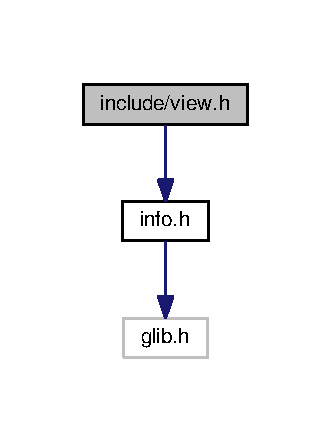
\includegraphics[width=159pt]{view_8h__incl}
\end{center}
\end{figure}
\subsection*{Funções}
\begin{DoxyCompactItemize}
\item 
\mbox{\Hypertarget{view_8h_ab13e858612c64eeef73aff1d8a03945e}\label{view_8h_ab13e858612c64eeef73aff1d8a03945e}} 
void \hyperlink{view_8h_ab13e858612c64eeef73aff1d8a03945e}{print\+Menu} ()
\begin{DoxyCompactList}\small\item\em Imprimir o menu. \end{DoxyCompactList}\item 
\mbox{\Hypertarget{view_8h_aa8165246642991f007f24facccf818ae}\label{view_8h_aa8165246642991f007f24facccf818ae}} 
void \hyperlink{view_8h_aa8165246642991f007f24facccf818ae}{print\+Separator} ()
\begin{DoxyCompactList}\small\item\em Imprimir um separador. \end{DoxyCompactList}\item 
\mbox{\Hypertarget{view_8h_ab319f92f61072f8a469f17f63c46f103}\label{view_8h_ab319f92f61072f8a469f17f63c46f103}} 
void \hyperlink{view_8h_ab319f92f61072f8a469f17f63c46f103}{clean\+Console} ()
\begin{DoxyCompactList}\small\item\em Limpar o terminal. \end{DoxyCompactList}\item 
\mbox{\Hypertarget{view_8h_afe00396766eb6b8ca4674de4c5d3d949}\label{view_8h_afe00396766eb6b8ca4674de4c5d3d949}} 
void \hyperlink{view_8h_afe00396766eb6b8ca4674de4c5d3d949}{reset\+Color} ()
\begin{DoxyCompactList}\small\item\em Resetar o texto à sua cor padrão. \end{DoxyCompactList}\item 
\mbox{\Hypertarget{view_8h_af7082af28af567c98aa48add7be13826}\label{view_8h_af7082af28af567c98aa48add7be13826}} 
void \hyperlink{view_8h_af7082af28af567c98aa48add7be13826}{bold\+Red} ()
\begin{DoxyCompactList}\small\item\em Colocar a vermelho o conteúdo impresso de seguida. \end{DoxyCompactList}\item 
\mbox{\Hypertarget{view_8h_a7a890c1f6b6e24b7a1b76f3286b08daf}\label{view_8h_a7a890c1f6b6e24b7a1b76f3286b08daf}} 
void \hyperlink{view_8h_a7a890c1f6b6e24b7a1b76f3286b08daf}{bold\+Cyan} ()
\begin{DoxyCompactList}\small\item\em Colocar a ciano o conteúdo impresso de seguida. \end{DoxyCompactList}\item 
\mbox{\Hypertarget{view_8h_abc3c807ccd9bbeacf64a401a08e31794}\label{view_8h_abc3c807ccd9bbeacf64a401a08e31794}} 
void \hyperlink{view_8h_abc3c807ccd9bbeacf64a401a08e31794}{view\+Print\+Start\+Values} (char $\ast$clients\+\_\+path, char $\ast$products\+\_\+path, char $\ast$sales\+\_\+path, int valid\+\_\+clients, int valid\+\_\+products, int valid\+\_\+sales, int clients\+\_\+read, int products\+\_\+read, int sales\+\_\+read)
\begin{DoxyCompactList}\small\item\em Imprimir os valores de carregamento da base de dados. \end{DoxyCompactList}\item 
void \hyperlink{view_8h_af8957d2f3430554a8f7e96d95f226875}{print\+Message} (char $\ast$)
\begin{DoxyCompactList}\small\item\em Imprime a mensagem fornecida. \end{DoxyCompactList}\item 
void \hyperlink{view_8h_ac541d0aad82b358134b66b2ad467efc6}{list\+View} (char $\ast$$\ast$, int, int)
\begin{DoxyCompactList}\small\item\em De um array de strings, mostra ao utilizador o conteúdo em forma de páginas. \end{DoxyCompactList}\item 
void \hyperlink{view_8h_a3b419a749ee7923cef5f973e6ff42da8}{table\+View} (int $\ast$$\ast$, char $\ast$)
\begin{DoxyCompactList}\small\item\em De um array de inteiros, mostra ao utilizador o conteúdo numa tabela. \end{DoxyCompactList}\item 
void \hyperlink{view_8h_a2ef14d61d6cdd26b9edd54edf25385f2}{querie1\+View} (char $\ast$, char $\ast$, char $\ast$)
\begin{DoxyCompactList}\small\item\em Função responsável por mostrar o resultado da query 1 ao utilizador. \end{DoxyCompactList}\item 
void \hyperlink{view_8h_ac34b7584c0643bf6408b66cc28b705e2}{querie2\+View} (char $\ast$$\ast$)
\begin{DoxyCompactList}\small\item\em Função responsável por mostrar o resultado da query 2 ao utilizador. \end{DoxyCompactList}\item 
void \hyperlink{view_8h_a852f0e5b13c5543dcb1911bd92326901}{querie3\+View} (double $\ast$, int, char $\ast$)
\begin{DoxyCompactList}\small\item\em Função responsável por mostrar o resultado da query 3 ao utilizador. \end{DoxyCompactList}\item 
void \hyperlink{view_8h_aa05f76592204f12ee6a8036110506f63}{querie4\+View} (char $\ast$$\ast$$\ast$, int, int, int $\ast$, int)
\begin{DoxyCompactList}\small\item\em Função responsável por mostrar o resultado da query 4 ao utilizador. \end{DoxyCompactList}\item 
void \hyperlink{view_8h_acee36c646ca408aa524b575bdd4e58bb}{querie5\+View} (char $\ast$$\ast$)
\begin{DoxyCompactList}\small\item\em Função responsável por mostrar o resultado da query 5 ao utilizador. \end{DoxyCompactList}\item 
void \hyperlink{view_8h_a78353553c9b19854cc30593f30e2f36f}{querie6\+View} (int $\ast$)
\begin{DoxyCompactList}\small\item\em Função responsável por mostrar o resultado da query 6 ao utilizador. \end{DoxyCompactList}\item 
void \hyperlink{view_8h_a5b80552d8dbaa3411b0509b6a2f6dd72}{querie7\+View} (int $\ast$$\ast$)
\begin{DoxyCompactList}\small\item\em Função responsável por mostrar o resultado da query 7 ao utilizador. \end{DoxyCompactList}\item 
void \hyperlink{view_8h_ae0b57d62eba799b970d009c05570d7a0}{querie8\+View} (\hyperlink{structquerie8Aux}{Query8\+Aux}, int, int)
\begin{DoxyCompactList}\small\item\em Função responsável por mostrar o resultado da query 8 ao utilizador. \end{DoxyCompactList}\item 
void \hyperlink{view_8h_a4c32ba440f89b84ce79d4c0bc680f9a9}{querie9\+View} (\hyperlink{structquerie9Aux}{Query9\+Aux} \hyperlink{structaux}{aux}, char type, int)
\begin{DoxyCompactList}\small\item\em Função responsável por mostrar o resultado da query 9 ao utilizador. \end{DoxyCompactList}\item 
void \hyperlink{view_8h_ae3c40a3cac022c97428ad533d6a88bbf}{querie10\+View} (\hyperlink{structinfo}{Info} $\ast$, int, char $\ast$, int)
\begin{DoxyCompactList}\small\item\em Função responsável por mostrar o resultado da query 10 ao utilizador. \end{DoxyCompactList}\item 
void \hyperlink{view_8h_aa73c108a62ffcabe908557747c7f3afa}{querie11\+View} (\hyperlink{structaux}{Aux} $\ast$, int, int)
\begin{DoxyCompactList}\small\item\em Função responsável por mostrar o resultado da query 11 ao utilizador. \end{DoxyCompactList}\item 
void \hyperlink{view_8h_a4d683ab642ad64b1099e1fb34bab8611}{querie12\+View} (\hyperlink{structmoney}{Money} $\ast$, int, char $\ast$, int)
\begin{DoxyCompactList}\small\item\em Função responsável por mostrar o resultado da query 12 ao utilizador. \end{DoxyCompactList}\end{DoxyCompactItemize}


\subsection{Descrição detalhada}
Módulo da view. 



\subsection{Documentação das funções}
\mbox{\Hypertarget{view_8h_ac541d0aad82b358134b66b2ad467efc6}\label{view_8h_ac541d0aad82b358134b66b2ad467efc6}} 
\index{view.\+h@{view.\+h}!list\+View@{list\+View}}
\index{list\+View@{list\+View}!view.\+h@{view.\+h}}
\subsubsection{\texorpdfstring{list\+View()}{listView()}}
{\footnotesize\ttfamily void list\+View (\begin{DoxyParamCaption}\item[{char $\ast$$\ast$}]{,  }\item[{int}]{,  }\item[{int}]{ }\end{DoxyParamCaption})}



De um array de strings, mostra ao utilizador o conteúdo em forma de páginas. 


\begin{DoxyParams}{Parâmetros}
{\em list} & Array de códigos de produtos \\
\hline
{\em size} & Tamanho do array \\
\hline
\end{DoxyParams}
\mbox{\Hypertarget{view_8h_af8957d2f3430554a8f7e96d95f226875}\label{view_8h_af8957d2f3430554a8f7e96d95f226875}} 
\index{view.\+h@{view.\+h}!print\+Message@{print\+Message}}
\index{print\+Message@{print\+Message}!view.\+h@{view.\+h}}
\subsubsection{\texorpdfstring{print\+Message()}{printMessage()}}
{\footnotesize\ttfamily void print\+Message (\begin{DoxyParamCaption}\item[{char $\ast$}]{ }\end{DoxyParamCaption})}



Imprime a mensagem fornecida. 


\begin{DoxyParams}{Parâmetros}
{\em message} & Mensagem a ser impressa \\
\hline
\end{DoxyParams}
\mbox{\Hypertarget{view_8h_ae3c40a3cac022c97428ad533d6a88bbf}\label{view_8h_ae3c40a3cac022c97428ad533d6a88bbf}} 
\index{view.\+h@{view.\+h}!querie10\+View@{querie10\+View}}
\index{querie10\+View@{querie10\+View}!view.\+h@{view.\+h}}
\subsubsection{\texorpdfstring{querie10\+View()}{querie10View()}}
{\footnotesize\ttfamily void querie10\+View (\begin{DoxyParamCaption}\item[{\hyperlink{structinfo}{Info} $\ast$}]{,  }\item[{int}]{,  }\item[{char $\ast$}]{,  }\item[{int}]{ }\end{DoxyParamCaption})}



Função responsável por mostrar o resultado da query 10 ao utilizador. 


\begin{DoxyParams}{Parâmetros}
{\em $\ast$info} & Array com os produtos mais comprados por um certo cliente \\
\hline
{\em n} & Tamanho do array com os produtos \\
\hline
{\em client} & Cliente ao qual as informações do array estão relacionadas \\
\hline
{\em page} & Página da lista que é para ser mostrada \\
\hline
\end{DoxyParams}
\mbox{\Hypertarget{view_8h_aa73c108a62ffcabe908557747c7f3afa}\label{view_8h_aa73c108a62ffcabe908557747c7f3afa}} 
\index{view.\+h@{view.\+h}!querie11\+View@{querie11\+View}}
\index{querie11\+View@{querie11\+View}!view.\+h@{view.\+h}}
\subsubsection{\texorpdfstring{querie11\+View()}{querie11View()}}
{\footnotesize\ttfamily void querie11\+View (\begin{DoxyParamCaption}\item[{\hyperlink{structaux}{Aux} $\ast$}]{,  }\item[{int}]{,  }\item[{int}]{ }\end{DoxyParamCaption})}



Função responsável por mostrar o resultado da query 11 ao utilizador. 


\begin{DoxyParams}{Parâmetros}
{\em result} & Lista com os top n produtos mais vendidos \\
\hline
{\em n} & Número de produtos a serem mostrados \\
\hline
{\em page} & Página da lista qque é para ser mostrada \\
\hline
\end{DoxyParams}
\mbox{\Hypertarget{view_8h_a4d683ab642ad64b1099e1fb34bab8611}\label{view_8h_a4d683ab642ad64b1099e1fb34bab8611}} 
\index{view.\+h@{view.\+h}!querie12\+View@{querie12\+View}}
\index{querie12\+View@{querie12\+View}!view.\+h@{view.\+h}}
\subsubsection{\texorpdfstring{querie12\+View()}{querie12View()}}
{\footnotesize\ttfamily void querie12\+View (\begin{DoxyParamCaption}\item[{\hyperlink{structmoney}{Money} $\ast$}]{,  }\item[{int}]{,  }\item[{char $\ast$}]{,  }\item[{int}]{ }\end{DoxyParamCaption})}



Função responsável por mostrar o resultado da query 12 ao utilizador. 


\begin{DoxyParams}{Parâmetros}
{\em list} & Lista com os top n produtos mais comprados por um certo cliente \\
\hline
{\em n} & Número de produtos a serem mostrados \\
\hline
{\em page} & Página da lista qque é para ser mostrada \\
\hline
\end{DoxyParams}
\mbox{\Hypertarget{view_8h_a2ef14d61d6cdd26b9edd54edf25385f2}\label{view_8h_a2ef14d61d6cdd26b9edd54edf25385f2}} 
\index{view.\+h@{view.\+h}!querie1\+View@{querie1\+View}}
\index{querie1\+View@{querie1\+View}!view.\+h@{view.\+h}}
\subsubsection{\texorpdfstring{querie1\+View()}{querie1View()}}
{\footnotesize\ttfamily void querie1\+View (\begin{DoxyParamCaption}\item[{char $\ast$}]{,  }\item[{char $\ast$}]{,  }\item[{char $\ast$}]{ }\end{DoxyParamCaption})}



Função responsável por mostrar o resultado da query 1 ao utilizador. 


\begin{DoxyParams}{Parâmetros}
{\em clients\+\_\+path} & Caminho para o ficheiro dos clients \\
\hline
{\em products\+\_\+path} & Caminho para o ficheiro dos produtos \\
\hline
{\em sales\+\_\+path} & Caminho para o ficheiro das vendas \\
\hline
\end{DoxyParams}
\mbox{\Hypertarget{view_8h_ac34b7584c0643bf6408b66cc28b705e2}\label{view_8h_ac34b7584c0643bf6408b66cc28b705e2}} 
\index{view.\+h@{view.\+h}!querie2\+View@{querie2\+View}}
\index{querie2\+View@{querie2\+View}!view.\+h@{view.\+h}}
\subsubsection{\texorpdfstring{querie2\+View()}{querie2View()}}
{\footnotesize\ttfamily void querie2\+View (\begin{DoxyParamCaption}\item[{char $\ast$$\ast$}]{ }\end{DoxyParamCaption})}



Função responsável por mostrar o resultado da query 2 ao utilizador. 


\begin{DoxyParams}{Parâmetros}
{\em list} & Array com os produtos inicializados com uma letra inicial especifica por ordem alfabética \\
\hline
\end{DoxyParams}
\mbox{\Hypertarget{view_8h_a852f0e5b13c5543dcb1911bd92326901}\label{view_8h_a852f0e5b13c5543dcb1911bd92326901}} 
\index{view.\+h@{view.\+h}!querie3\+View@{querie3\+View}}
\index{querie3\+View@{querie3\+View}!view.\+h@{view.\+h}}
\subsubsection{\texorpdfstring{querie3\+View()}{querie3View()}}
{\footnotesize\ttfamily void querie3\+View (\begin{DoxyParamCaption}\item[{double $\ast$}]{,  }\item[{int}]{,  }\item[{char $\ast$}]{ }\end{DoxyParamCaption})}



Função responsável por mostrar o resultado da query 3 ao utilizador. 


\begin{DoxyParams}{Parâmetros}
{\em products} & Array com valores totais de vendas e faturado de um certo produtos globalmente ou dividido por filial \\
\hline
{\em int} & Escolha do utilizador se pretende ver os resultados globalmente ou dividido filial a filial \\
\hline
{\em char$\ast$} & Código do produto ao qual as informações pertencem \\
\hline
\end{DoxyParams}
\mbox{\Hypertarget{view_8h_aa05f76592204f12ee6a8036110506f63}\label{view_8h_aa05f76592204f12ee6a8036110506f63}} 
\index{view.\+h@{view.\+h}!querie4\+View@{querie4\+View}}
\index{querie4\+View@{querie4\+View}!view.\+h@{view.\+h}}
\subsubsection{\texorpdfstring{querie4\+View()}{querie4View()}}
{\footnotesize\ttfamily void querie4\+View (\begin{DoxyParamCaption}\item[{char $\ast$$\ast$$\ast$}]{,  }\item[{int}]{,  }\item[{int}]{,  }\item[{int $\ast$}]{,  }\item[{int}]{ }\end{DoxyParamCaption})}



Função responsável por mostrar o resultado da query 4 ao utilizador. 


\begin{DoxyParams}{Parâmetros}
{\em products} & Array com produtos que nínguem comprou ordenados por ordem alfabética \\
\hline
{\em global} & Escolha do utilizador se pretende ver globalmente ou separado por filiais \\
\hline
{\em branch} & Número da filial escolhida \\
\hline
{\em size} & Tamanho do array dos produtos \\
\hline
\end{DoxyParams}
\mbox{\Hypertarget{view_8h_acee36c646ca408aa524b575bdd4e58bb}\label{view_8h_acee36c646ca408aa524b575bdd4e58bb}} 
\index{view.\+h@{view.\+h}!querie5\+View@{querie5\+View}}
\index{querie5\+View@{querie5\+View}!view.\+h@{view.\+h}}
\subsubsection{\texorpdfstring{querie5\+View()}{querie5View()}}
{\footnotesize\ttfamily void querie5\+View (\begin{DoxyParamCaption}\item[{char $\ast$$\ast$}]{ }\end{DoxyParamCaption})}



Função responsável por mostrar o resultado da query 5 ao utilizador. 


\begin{DoxyParams}{Parâmetros}
{\em clients} & Array com os clients que compraram em todas as filiais \\
\hline
\end{DoxyParams}
\mbox{\Hypertarget{view_8h_a78353553c9b19854cc30593f30e2f36f}\label{view_8h_a78353553c9b19854cc30593f30e2f36f}} 
\index{view.\+h@{view.\+h}!querie6\+View@{querie6\+View}}
\index{querie6\+View@{querie6\+View}!view.\+h@{view.\+h}}
\subsubsection{\texorpdfstring{querie6\+View()}{querie6View()}}
{\footnotesize\ttfamily void querie6\+View (\begin{DoxyParamCaption}\item[{int $\ast$}]{ }\end{DoxyParamCaption})}



Função responsável por mostrar o resultado da query 6 ao utilizador. 


\begin{DoxyParams}{Parâmetros}
{\em list} & Array com os valores totais dos clientes que que não realizaram compras e dos produtos que não foram comprados \\
\hline
\end{DoxyParams}
\mbox{\Hypertarget{view_8h_a5b80552d8dbaa3411b0509b6a2f6dd72}\label{view_8h_a5b80552d8dbaa3411b0509b6a2f6dd72}} 
\index{view.\+h@{view.\+h}!querie7\+View@{querie7\+View}}
\index{querie7\+View@{querie7\+View}!view.\+h@{view.\+h}}
\subsubsection{\texorpdfstring{querie7\+View()}{querie7View()}}
{\footnotesize\ttfamily void querie7\+View (\begin{DoxyParamCaption}\item[{int $\ast$$\ast$}]{ }\end{DoxyParamCaption})}



Função responsável por mostrar o resultado da query 7 ao utilizador. 


\begin{DoxyParams}{Parâmetros}
{\em totals} & Valores totais dos produtos comprados separados por mês de um certo cliente \\
\hline
\end{DoxyParams}
\mbox{\Hypertarget{view_8h_ae0b57d62eba799b970d009c05570d7a0}\label{view_8h_ae0b57d62eba799b970d009c05570d7a0}} 
\index{view.\+h@{view.\+h}!querie8\+View@{querie8\+View}}
\index{querie8\+View@{querie8\+View}!view.\+h@{view.\+h}}
\subsubsection{\texorpdfstring{querie8\+View()}{querie8View()}}
{\footnotesize\ttfamily void querie8\+View (\begin{DoxyParamCaption}\item[{\hyperlink{structquerie8Aux}{Query8\+Aux}}]{,  }\item[{int}]{,  }\item[{int}]{ }\end{DoxyParamCaption})}



Função responsável por mostrar o resultado da query 8 ao utilizador. 


\begin{DoxyParams}{Parâmetros}
{\em aux} & Array com as totais de vendas e unidades vendidas num intervalo de meses \\
\hline
{\em first} & Primeiro mês do intervalo \\
\hline
{\em second} & Ultimo mês do intervalo \\
\hline
\end{DoxyParams}
\mbox{\Hypertarget{view_8h_a4c32ba440f89b84ce79d4c0bc680f9a9}\label{view_8h_a4c32ba440f89b84ce79d4c0bc680f9a9}} 
\index{view.\+h@{view.\+h}!querie9\+View@{querie9\+View}}
\index{querie9\+View@{querie9\+View}!view.\+h@{view.\+h}}
\subsubsection{\texorpdfstring{querie9\+View()}{querie9View()}}
{\footnotesize\ttfamily void querie9\+View (\begin{DoxyParamCaption}\item[{\hyperlink{structquerie9Aux}{Query9\+Aux}}]{aux,  }\item[{char}]{type,  }\item[{int}]{ }\end{DoxyParamCaption})}



Função responsável por mostrar o resultado da query 9 ao utilizador. 


\begin{DoxyParams}{Parâmetros}
{\em aux} & Array com os clientes qe compraram certo produto nas diferentes filiais \\
\hline
{\em type} & Tipo de vendas \\
\hline
{\em page} & Página da lista que é para ser mostrada \\
\hline
\end{DoxyParams}
\mbox{\Hypertarget{view_8h_a3b419a749ee7923cef5f973e6ff42da8}\label{view_8h_a3b419a749ee7923cef5f973e6ff42da8}} 
\index{view.\+h@{view.\+h}!table\+View@{table\+View}}
\index{table\+View@{table\+View}!view.\+h@{view.\+h}}
\subsubsection{\texorpdfstring{table\+View()}{tableView()}}
{\footnotesize\ttfamily void table\+View (\begin{DoxyParamCaption}\item[{int $\ast$$\ast$}]{,  }\item[{char $\ast$}]{ }\end{DoxyParamCaption})}



De um array de inteiros, mostra ao utilizador o conteúdo numa tabela. 


\begin{DoxyParams}{Parâmetros}
{\em list} & Array de quantidades de produtos comprados nos meses \\
\hline
{\em client} & Código do cliente ao qual as quantidades estão relacionadas \\
\hline
\end{DoxyParams}

\hypertarget{main_8c}{}\section{Referência ao ficheiro src/main.c}
\label{main_8c}\index{src/main.\+c@{src/main.\+c}}


Ficheiro principal.  


{\ttfamily \#include \char`\"{}args.\+h\char`\"{}}\newline
{\ttfamily \#include \char`\"{}controller.\+h\char`\"{}}\newline
Diagrama de dependências de inclusão para main.\+c\+:
\nopagebreak
\begin{figure}[H]
\begin{center}
\leavevmode
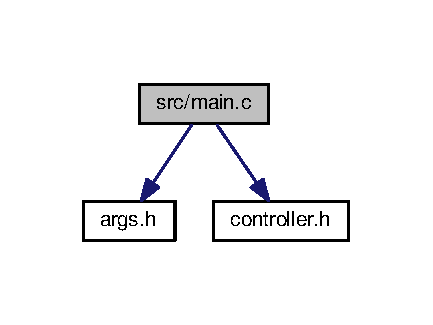
\includegraphics[width=208pt]{main_8c__incl}
\end{center}
\end{figure}
\subsection*{Funções}
\begin{DoxyCompactItemize}
\item 
\mbox{\Hypertarget{main_8c_a0ddf1224851353fc92bfbff6f499fa97}\label{main_8c_a0ddf1224851353fc92bfbff6f499fa97}} 
int \hyperlink{main_8c_a0ddf1224851353fc92bfbff6f499fa97}{main} (int argc, char $\ast$argv\mbox{[}$\,$\mbox{]})
\begin{DoxyCompactList}\small\item\em Função principal. \end{DoxyCompactList}\end{DoxyCompactItemize}


\subsection{Descrição detalhada}
Ficheiro principal. 


%--- End generated contents ---

% Index
\backmatter
\newpage
\phantomsection
\clearemptydoublepage
\addcontentsline{toc}{chapter}{Índice}
\printindex

\end{document}
